\documentclass[12pt,a4paper]{report}

% ─── Pakete ────────────────────────────────────────────────────────────────────
\usepackage[utf8]{inputenc}
\usepackage[T1]{fontenc}
\usepackage[ngerman]{babel}
\usepackage{geometry}

\usepackage{amsmath, amssymb, amsthm, mathtools}
\usepackage{graphicx}
\usepackage{booktabs}
\usepackage{array}
\usepackage{longtable}
\usepackage{hyperref}
\usepackage{xcolor}
\usepackage{enumitem}
\usepackage{setspace}
\usepackage{caption}
\captionsetup{width=\linewidth, singlelinecheck=false}
\usepackage{fancyhdr}
\usepackage{parskip}
\usepackage{lmodern}
\usepackage[expansion=false]{microtype}
\usepackage{microtype}

\setlist[itemize,1]{label=--}

% ─── Layout ────────────────────────────────────────────────────────────────────
\geometry{margin=2.5cm}

\hypersetup{colorlinks=true, linkcolor=[rgb]{0.0,0.3,0.6},
	citecolor=[rgb]{0.0,0.3,0.6}, urlcolor=[rgb]{0.0,0.3,0.6}}


% ─── Theorem-Umgebungen ────────────────────────────────────────────────────────
\theoremstyle{plain}
\newtheorem{theorem}{Theorem}[section]
\newtheorem{lemma}[theorem]{Lemma}
\newtheorem{korollar}[theorem]{Korollar}
\newtheorem{proposition}[theorem]{Proposition}

\theoremstyle{definition}
\newtheorem{definition}[theorem]{Definition}
\newtheorem{experiment}[theorem]{Experiment}
\newtheorem{axiom}[theorem]{Axiom}
\newtheorem{beobachtung}[theorem]{Beobachtung}

\theoremstyle{remark}
\newtheorem{bemerkung}[theorem]{Bemerkung}
\newtheorem{beispiel}[theorem]{Beispiel}

% ─── Mathe-Operatoren ──────────────────────────────────────────────────────────
\DeclareMathOperator{\WZI}{WZI}
\DeclareMathOperator{\IZI}{IZI}
\DeclareMathOperator{\EC}{EC}
\DeclareMathOperator{\PAC}{PAC}
\DeclareMathOperator{\sgn}{sgn}
\DeclareMathOperator{\rot}{rot}

\title{\textbf{Die epistemische Wolke,\\ der unsichtbare Geist des Lebens\\ und die Rechtsdrehung kortikaler Informationsverarbeitung}}
\author{Stephan Epp}
\date{12. März 2026}

% ══════════════════════════════════════════════════════════════════════════════
\begin{document}
	% ─── Titelseite ────────────────────────────────────────────────────────────────
	\maketitle	
	% ─── Inhaltsverzeichnis ────────────────────────────────────────────────────────
	\tableofcontents
	\newpage
	
	% ══════════════════════════════════════════════════════════════════════════════
	\chapter{Einleitung}
	% ══════════════════════════════════════════════════════════════════════════════
	Das Gehirn des Menschen, dem die ganze Wahrheit verborgen ist,
	befindet sich wie in einer Wolke. Er ist im Denken nicht immer
	ganz frei und hat keinen vollständigen Zugang zu allen Informationen,
	die eine umfassende Lösung erfordert. Das Gehirn benötigt für seine Funktion den \emph{unsichtbaren
		Geist des Lebens} -- die elektro-chemische Informationsübertragung
	von Synapse zu Synapse. Dieser Geist allein gibt die ganze Wahrheit über alle Bereiche und Fragen des Lebens.
	Die Informationsverarbeitung im Gehirn verläuft
	\textbf{rechtsdrehend} -- von oben betrachtet im Uhrzeigersinn. Die Ad-hoc-Informationsbereitstellung und Selektion nach Bedarf
	erfolgt \textbf{selektiv} und ist an die Intaktheit des
	Lebensgeistflusses gebunden.
	
	Die vorliegende Abhandlung -- eine wesentlich erweiterte und vertieft
	ausgearbeitete Fassung früherer Arbeiten des Autors -- vereint vier
	fundamentale Beobachtungen über Kognition, Neurobiologie und die
	Physik des Denkens zu einem kohärenten theoretischen Rahmen.
	
	\textbf{Erste Kernaussage:} Ein Mensch, dem die ganze Wahrheit verborgen
	ist, befindet sich im kognitiven Zustand einer \emph{epistemischen Wolke}.
	Dieser Zustand ist nicht blo\ss{} ein philosophisches Konstrukt, sondern
	eine neurobiologisch messbare Realität: veränderte präfrontale
	Konnektivität, supprimierte Gamma-Kohärenz, erhöhte Amygdala-Reaktivität
	und chronisch erhöhte Cortisol-Spiegel sind ihre biologischen Signaturen.
	
	\textbf{Zweite Kernaussage:} Das Gehirn benötigt für seine Funktion
	den \emph{unsichtbaren Geist des Lebens} -- den kontinuierlichen, elektro-chemischen
	Impulsfluss von Synapse zu Synapse. Dieser Fluss -- in seiner biologischen
	Manifestation als Aktionspotential, Neurotransmitter-Quantenfreisetzung und
	synaptische Plastizität -- ist der einzige Kanal, durch den die ganze
	Wahrheit das Bewusstsein erreichen kann.
	
	\textbf{Dritte Kernaussage (neu in dieser Fassung):} Die Informationsverarbeitung
	im Gehirn des Menschen verläuft \emph{rechtsdrehend} -- von oben (dorsal)
	betrachtet im Uhrzeigersinn. Dies bedeutet: die kortikale Aktivierungswelle
	propagiert von anterior zu lateral-rechts, zu posterior, zu lateral-links
	und zurück nach anterior. Diese Rechtsdrehung ist die kinematische
	Grundeigenschaft des gesunden Lebensgeistflusses und lässt sich formal
	durch negative Winkelgeschwindigkeit, Phasen-Führungs-Analyse und
	Phase-Amplitude-Coupling nachweisen.
	
	\textbf{Vierte Kernaussage (neu in dieser Fassung):} Die
	Ad-hoc-Informationsbereitstellung -- die Selektion relevanter Gedächtnisinhalte
	\emph{nach Bedarf} im Moment der Anforderung -- erfolgt selektiv und ist
	an die Intaktheit des rechtsdrehenden Lebensgeistflusses gebunden. Die
	epistemische Wolke stört diese Selektion und liefert entweder falsche,
	irrelevante oder gar keine Informationen zum Zeitpunkt der Anforderung.
	
	Zur Unterstützung dieser vier Thesen werden neun Klassen
	computergestützter Modellexperimente mit insgesamt \textbf{33 Teildiagrammen}
	präsentiert, begleitet von \textbf{sieben Theoremen mit vollständigen Beweisen},
	\textbf{fünf Definitionen}, \textbf{drei Axiomen} und
	\textbf{zwei formalen Propositionen}.
	
	\textbf{Schlüsselwörter:}
	Epistemische Wolke, Lebensgeist, Synaptische Informationsübertragung,
	Aktionspotential, Rechtsdrehung kortikaler Aktivität, negative Winkelgeschwindigkeit,
	Phase-Amplitude-Coupling, selektiver Informationsabruf, Ad-hoc-Selektion,
	kognitive Freiheit, Wahrheitszugang, Default Mode Network, STDP,
	Bayesianische Kognition, Neurotransmitter-Balance, transgenerationale Epigenetik,
	Thalamus-ARAS-System, Cortisol-HPA-Achse
	
	\section{Hintergrund und Problemstellung}
	
	Das menschliche Denken ist kein monolithisches Phänomen. Es besitzt
	eine biologische Architektur, eine informationstheoretische Struktur,
	eine kinematische Eigenschaft und eine selektive Dynamik. Diese vier
	Dimensionen -- (1)~epistemische Vollständigkeit, (2)~Lebens\-geist-Intensität,
	(3)~kortikale Drehrichtung und (4)~selektive Bereitstellung -- sind
	untrennbar miteinander verwoben.
	
	Die Kernbeobachtung, die diese Arbeit antreibt, ist gleichzeitig intuitiv
	und biologisch präzise: Ein Mensch, dessen Geist in einer epistemischen
	Wolke eingeschlossen ist, denkt nicht frei. Er löst Probleme unvollständig,
	weil er wesentliche Informationen nicht verfügbar hat -- nicht nur,
	weil sie ihm vorenthalten werden, sondern weil die Wolke selbst den
	neurobiologischen Mechanismus des Zugangs stört.
	
	\section{Dimension: Epistemische Vollständigkeit}
	
	Platon beschrieb im Höhlengleichnis Menschen, die Schatten für die
	Wirklichkeit halten. Heute können wir diese Intuition biologisch präzisieren:
	Das Gehirn einer Person, die nur Schatten der Wahrheit kennt, arbeitet
	unter suboptimaler präfrontaler Aktivität, erhöhter amygdalarer
	Kontrolle und reduzierter synaptischer Plastizität. Die Wolke ist
	nicht metaphorisch -- sie ist neurochemisch.
	
	Entscheidend ist: Es genügt nicht, dass eine Person
	\emph{möchte}, frei zu denken. Das Gehirn kann nicht vollständig
	frei denken, wenn die notwendigen Informationen nicht vorhanden sind.
	Die kognitive Freiheit ist keine rein willentliche Kapazität, sondern
	eine Funktion des Informationszugangs und der Lebensgeist-Intensität.
	
	\section{Dimension: Der unsichtbare Geist des Lebens}
	
	Wenn Philosophen und Theologen durch die Jahrhunderte von einem ``Geist''
	sprachen, der im Körper wohnt und Denken ermöglicht, beschrieben
	sie -- ohne es zu wissen -- den elektro-chemischen Impulsfluss des
	Nervensystems. Luigi Galvani zeigte 1791 durch seine berühmten
	Froschschenkel-Experimente, dass Nerven durch Elektrizität aktiviert
	werden. Alan Hodgkin und Andrew Huxley formalisierten 1952 die exakte
	Mathematik dieses ``Geistes'': das Aktionspotential.
	
	Dieser unsichtbare Geist ist deshalb unsichtbar, weil er sich unterhalb
	der Wahrnehmungsschwelle abspielt: Ein einzelnes Aktionspotential dauert
	$\approx 1$\,ms und ist $\approx 100$\,mV stark -- weit unterhalb jeder
	makroskopischen Beobachtbarkeit. Und doch ist er die Ursprache des Denkens,
	die Trägerwelle aller Information, der Strom, in dem die Wahrheit flie\ss{}t.
	
	\section{Dimension: Rechtsdrehende Verarbeitung}
	
	Eine bisher wenig formalisierte, aber biologisch bedeutsame Beobachtung
	ist, dass die Aktivierungswellen des menschlichen Kortex eine bevorzugte
	\emph{Drehrichtung} aufweisen. Von dorsal (oben) betrachtet propagiert
	die kortikale Aktivierungswelle im Uhrzeigersinn -- also rechtsdrehend.
	
	Diese Beobachtung ist nicht trivial. Sie impliziert, dass das Gehirn
	eine intrinsische \emph{Chiralität} der Informationsverarbeitung besitzt --
	eine Asymmetrie, die tief mit der hemisphärischen Lateralisierung,
	der thalamo-kortikalen Schleifenarchitektur und der Richtung
	zerebraler Blutfluss-Rotationsmuster zusammenhängt.
	
	\section{Dimension: Selektive Ad-hoc-Bereitstellung}
	
	Das Gedächtnis ist kein passiver Speicher. Es ist ein aktives,
	prädiktives System, das Informationen \emph{nach Bedarf} und
	\emph{zum Zeitpunkt der Anforderung} bereitstellt. Diese Selektion --
	hier als \emph{Ad-hoc-Informationsbereitstellung} (AIB) bezeichnet --
	erfordert ein intaktes thalamo-kortikales Gateway (ARAS-System),
	funktionale prefrontale Exekutivkontrolle und -- entscheidend --
	einen aktiven, rechtsdrehenden Lebensgeistfluss.
	
	Wenn die epistemische Wolke diesen Fluss stört, bricht die Selektion
	zusammen: Das Gehirn liefert inkorrekte, verzerrte oder überhaupt
	keine Informationen zum richtigen Zeitpunkt. Die Konsequenz ist nicht nur
	Unwissen -- es ist aktives Fehlinformiert-Sein.
	
	\section{Wichtige Bereiche für das Gehirn}
	Welche drei Bereiche sind am besten für das Gehirn? Die Freude, der Friede, die Freiheit. Die Freiheit ist der wichtigste Bereich, denn nur in der Freiheit und weniger in der Ordnung im Gehirn, bleibt die wirkliche Freiheit im Denken bestehen und erhalten. Zu wissen davon, dass du von allem, was du hast, auch viel hast, dass du gar nicht hast, ist Freiheit im Denken. Freude hat der Mensch zum Beispiel durch Erfolg bei der Arbeit oder durch gutes Essen. Nach dem Stuhlgang ist das Gehirn beruhigt.
	
	% ══════════════════════════════════════════════════════════════════════════════
	\chapter{Definitionen, Axiome und Theoreme}
	% ══════════════════════════════════════════════════════════════════════════════
	
	\section{Grundlegende Definitionen}
	
	
	\noindent\textbf{Definition 3.1: Epistemische Wolke (EC)}

		Eine Person $P$ befindet sich in einer epistemischen Wolke
		$\mathcal{W}$ bezüglich Problemraum $\Omega$, wenn ihre verfügbare
		Informationsmenge $\mathcal{I}_P$ vom notwendigen Set $\mathcal{I}^*$
		abweicht. Die \emph{Wolken-Dichte} ist:
		\[
		\delta(\mathcal{W}) \;:=\; 1 \;-\;
		\frac{|\mathcal{I}_P \,\cap\, \mathcal{I}^*|}{|\mathcal{I}^*|}
		\;\in\; [0,\,1].
		\]
		Für $\delta = 0$: vollständige Klarheit. Für $\delta = 1$: vollständige Blockade.

	
	
	\noindent\textbf{Definition 3.2: Unsichtbarer Geist des Lebens (UGL)}

		Der unsichtbare Geist des Lebens $\mathcal{G}$ ist der integrale
		Strom synaptischer Informationsübertragungsereignisse:
		\[
		\mathcal{G}(\mathcal{N}, t)
		\;:=\; \sum_{s \,\in\, \mathcal{S}}
		\lambda_s(t)\cdot w_s \cdot \phi_s,
		\]
		mit Aktionspotential-Frequenz $\lambda_s(t)$ [Hz], synaptischem Gewicht
		$w_s$ und Effizienz $\phi_s \in [0,1]$.

	
	
	\noindent\textbf{Definition 3.3: Rechtsdrehender Lebensgeist}

		\label{def:rechtsdrehend}
		Der Lebensgeist $\mathcal{G}$ ist \emph{rechtsdrehend} (Uhrzeigersinn,
		von dorsal betrachtet), wenn seine instantane Winkelgeschwindigkeit
		$\omega(t)$ des kortikalen Aktivierungsvektors $\vec{A}(t)$ durchgehend
		negativ ist:
		\[
		\omega(t) \;:=\; \frac{d}{dt}\,\arg\bigl(\vec{A}(t)\bigr)
		\;<\; 0 \quad \forall\, t \in [0, T].
		\]
		äquivalent: Die Phase $\varphi(t)$ des analytischen Signals nimmt
		monoton ab: $\dot{\varphi}(t) < 0$.

	
	
	\noindent\textbf{Definition 3.4: Ad-hoc-Informationsbereitstellung (AIB)}

		\label{def:aib}
		Die Ad-hoc-Informationsbereitstellung ist die Funktion
		$\mathcal{A}: \mathcal{Q} \times \mathcal{M} \to \mathcal{I}$,
		die zu einer Anfrage $q \in \mathcal{Q}$ aus dem Gedächtnis $\mathcal{M}$
		eine relevante Informationsmenge $\mathcal{I}_{q}$ selektiert:
		\[
		\mathcal{A}(q, \mathcal{M})
		\;:=\;
		\arg\max_{I \subseteq \mathcal{M}}
		\;\mathrm{Rel}(I, q) \cdot \mathrm{Avail}(I, \mathcal{G}),
		\]
		wobei $\mathrm{Rel}(I,q)$ die Relevanz von $I$ für $q$
		und $\mathrm{Avail}(I, \mathcal{G}) \in [0,1]$ die Verfügbarkeit
		unter aktuellem Lebensgeist-Niveau $\mathcal{G}$ ist.

	
	
	\noindent\textbf{Definition 3.5: Wahrheitszugang-Index (WZI)}

		\[
		\WZI(P,\,\mathcal{G},\,\mathcal{W})
		\;:=\;
		\bigl(1 - \delta(\mathcal{W})\bigr)
		\;\cdot\;
		\frac{\mathcal{G}(\mathcal{N},t)}{\mathcal{G}_{\max}}
		\;\cdot\;
		\mathbf{1}_{\omega < 0},
		\]
		wobei $\mathbf{1}_{\omega < 0}$ der Indikator für rechtsdrehenden
		Lebensgeist ist. Der Faktor $\mathbf{1}_{\omega < 0}$ kodiert, dass
		volles Wahrheitspotential nur im rechtsdrehenden Zustand erreichbar ist.

	
	\section{Axiome}
	
	
	\noindent\textbf{Axiom 3.1: Lebensgeist als notwendige Bedingung}

		$\mathcal{G} = 0 \implies \WZI = 0$.
		Maximaler Wahrheitszugang:
		$\WZI = 1 \iff \delta = 0 \;\wedge\; \mathcal{G} = \mathcal{G}_{\max}
		\;\wedge\; \omega < 0$.

	
	
	\noindent\textbf{Axiom 3.2: Rechtsdrehungs-Axiom}

		Der gesunde menschliche Kortex verarbeitet Information überwiegend
		im rechtsdrehenden Modus: $\Pr[\omega(t) < 0] > \Pr[\omega(t) > 0]$
		im wachen, klar denkenden Zustand.
		Die epistemische Wolke invertiert oder destabilisiert diese Präferenz.

	
	
	\noindent\textbf{Axiom 3.3: Selektivitäts-Axiom}

		Die Ad-hoc-Informationsbereitstellung ist \emph{selektiv} und nicht
		vollständig: $|\mathcal{A}(q,\mathcal{M})| \ll |\mathcal{M}|$.
		Die Qualität der Selektion ist monoton wachsend in $\mathcal{G}$
		und monoton fallend in $\delta(\mathcal{W})$.

	
	\section{Theoreme mit Beweisen}
	
	
	\noindent\textbf{Theorem 3.1: Informations-Notwendigkeits-Theorem}

		\[
		Q(P, \Omega) \;\leq\; \WZI(P, \mathcal{G}, \mathcal{W}).
		\]

	
	\begin{proof}
		Eine Lösung $\ell$ ist eine Abbildung $\mathcal{I}_P \cap \mathcal{I}^* \to \mathcal{A}$.
		Da $|\mathcal{I}_P \cap \mathcal{I}^*| \leq |\mathcal{I}^*|$, ist $Q \leq (1-\delta)$.
		Da die Verarbeitung synaptischen Fluss erfordert, gilt $Q \leq (1-\delta)\cdot\mathcal{G}/\mathcal{G}_{\max}$.
		Da maximale Effizienz nur im rechtsdrehenden Modus erreicht wird
		(Axiom~3.2), folgt $Q \leq \WZI$. 
	\end{proof}
	
	
	\noindent\textbf{Theorem 3.2: Wolken-Suppressions-Theorem}

		$d\mathcal{G}/d\delta \leq 0$:
		Eine dichtere Wolke supprimiert den Lebensgeist.

	
	\begin{proof}
		$c(\delta)$ = Cortisolspiegel (steigt mit $\delta$: $dc/d\delta > 0$).
		Cortisol reduziert synaptische Dichte: $d\mathcal{G}/dc < 0$.
		Kettenregel: $d\mathcal{G}/d\delta < 0$. 
	\end{proof}
	
	
	\noindent\textbf{Theorem 3.3: Rechtsdrehungs-Theorem (Kinematik)}

		\label{thm:rechts}
		Im gesunden wachen Gehirn gilt für den kortikalen Aktivierungsvektor
		$\vec{A}(t) = (A_x(t),\, A_y(t))$:
		\[
		\omega(t) \;=\;
		\frac{A_x(t)\,\dot{A}_y(t) - A_y(t)\,\dot{A}_x(t)}
		{|\vec{A}(t)|^2}
		\;<\; 0.
		\]

	
	\begin{proof}
		Das kortikale Aktivierungsfeld lässt sich als komplexwertige Funktion
		$\mathcal{A}(t) = A_x(t) + i\,A_y(t)$ schreiben.
		Im analytischen Signal (Hilbert-Transformation) ist die Instantanfrequenz:
		$\omega(t) = d\varphi/dt = \Im\bigl[\dot{\mathcal{A}} / \mathcal{A}\bigr]$.
		Im rechtsdrehenden Fall nimmt $\varphi$ ab: $d\varphi/dt < 0$.
		Die Kreuzprodukt-Formel $\omega = (A_x\dot{A}_y - A_y\dot{A}_x)/|\vec{A}|^2$
		ergibt sich direkt aus der Zeitableitung von $\varphi = \arctan(A_y/A_x)$:
		$\dot{\varphi} = (A_x\dot{A}_y - A_y\dot{A}_x)/(A_x^2+A_y^2)$. 
	\end{proof}
	
	
	\noindent\textbf{Theorem 3.4: Selektivitäts-Effizienz-Theorem}

		\label{thm:selektion}
		Die Ad-hoc-Selektionseffizienz $\eta_{\mathcal{A}}$ -- definiert als
		Anteil korrekt bereitgestellter relevanter Items -- ist beschränkt durch:
		\[
		\eta_{\mathcal{A}}(q, \mathcal{M}, \mathcal{G}, \delta)
		\;\leq\;
		\frac{\mathcal{G}}{\mathcal{G}_{\max}} \cdot (1-\delta)
		\;=\; \WZI.
		\]

	
	\begin{proof}
		$\mathcal{A}$ erfordert zwei Schritte: (i)~Zugang zum Gedächtnis $\mathcal{M}$
		(blockiert durch $\delta$: effektiver Zugang $(1-\delta)\cdot|\mathcal{M}|$);
		(ii)~Relevanz-Selektion über PFC-Exekutivkontrolle (proportional zu $\mathcal{G}/\mathcal{G}_{\max}$).
		Da beide Schritte sequenziell sind:
		$\eta_{\mathcal{A}} \leq (1-\delta) \cdot \mathcal{G}/\mathcal{G}_{\max} = \WZI$. 
	\end{proof}
	
	
	\noindent\textbf{Theorem 3.5: Doppelte Blockade (Korollar)}

		Die epistemische Wolke blockiert den Wahrheitszugang superlinear:
		\[
		\Delta\WZI \;\geq\; \delta + \varepsilon(\delta), \quad \varepsilon > 0,
		\]
		da sie sowohl $\delta$ direkt erhöht als auch $\mathcal{G}$ supprimiert
		und die Rechtsdrehung $(\omega < 0)$ destabilisiert.

	
	\begin{proof}
		Aus Theorem~3.2: $\mathcal{G}$ fällt mit $\delta$.
		Aus Axiom~3.2: $\Pr[\omega < 0]$ fällt mit $\delta$.
		Damit sind alle drei Faktoren in $\WZI$ gleichzeitig negativ betroffen,
		der Gesamtverlust ist streng grö\ss{}er als der direkte Verlust $\delta$. 
	\end{proof}
	
	
	\noindent\textbf{Theorem 3.6: Phasen-Führungs-Theorem (Rechtsdrehung)}

		\label{thm:phasenfuehr}
		Im rechtsdrehenden Kortex gilt für zwei Elektroden $i, j$
		mit Positionen $\theta_i < \theta_j$ (im Uhrzeigersinn gemessen):
		\[
		\Delta\varphi_{ij} \;:=\; \varphi_i(t) - \varphi_j(t) \;>\; 0,
		\]
		d.\,h.\ die frontale (frühere) Elektrode \emph{führt} die
		posteriore (spätere) in der Phase. Das Vorzeichen kehrt sich bei
		epistemischer Wolke (Desynchronisation).

	
	\begin{proof}
		Im rechtsdrehenden System propagiert die Aktivierungswelle mit konstanter
		Winkelgeschwindigkeit $\omega < 0$.
		Für Position $\theta_j > \theta_i$ (Uhrzeigersinn) gilt:
		$\varphi_j(t) = \varphi_i(t) - |\omega|\cdot(\theta_j - \theta_i)/v$,
		wobei $v$ die Ausbreitungsgeschwindigkeit ist.
		Damit $\Delta\varphi_{ij} = \varphi_i - \varphi_j = |\omega|(\theta_j-\theta_i)/v > 0$. 
	\end{proof}
	
	
	\noindent\textbf{Theorem 3.7: ARAS-Selektions-Theorem}

		\label{thm:aras}
		Das thalamo-kortikale ARAS-System öffnet seinen Informations-Gateway
		nur dann vollständig, wenn das kortikale Lebensgeist-Niveau $\mathcal{G}$
		eine Schwelle $\mathcal{G}_{\theta}$ überschreitet:
		\[
		\mathrm{Avail}(I, \mathcal{G})
		\;=\;
		\sigma\!\left(\frac{\mathcal{G} - \mathcal{G}_\theta}{\tau_\mathcal{G}}\right),
		\]
		mit der Sigmoid-Funktion $\sigma$, Schwelle $\mathcal{G}_\theta$ und
		Steilheit $\tau_\mathcal{G}$.
		Epistemische Wolke senkt $\mathcal{G}$ unter $\mathcal{G}_\theta$
		und schlie\ss{}t damit den Gateway.

	
	\begin{proof}
		Die thalamo-kortikale Ãœbertragung folgt einem Schwellenmechanismus:
		Unterhalb $\mathcal{G}_\theta$ dominiert tonische Inhibition durch
		Retikuläre-Formation-GABAerge Zellen, das heißt $\mathrm{Avail} \to 0$;
		oberhalb öffnet sich der Relay-Modus, das heißt $\mathrm{Avail} \to 1$.
		Die Sigmoid-Form folgt aus dem Boltzmann-Faktor der Kanaldynamik. 
	\end{proof}
	
	% ══════════════════════════════════════════════════════════════════════════════
	\chapter{Unsichtbarer Lebensgeist}
	% ══════════════════════════════════════════════════════════════════════════════
	
	\section{Das Aktionspotential -- wichtiger Lebensimpuls}
	
	Das Aktionspotential ist der kleinste, unteilbare Impuls des
	unsichtbaren Lebensgeistes. Es ist die physische Realisierung jedes
	Gedankens, jeder Erinnerung, jeder Entscheidung.
	
	\textbf{Die Biophysik im Detail.}
	Im Ruhezustand beträgt das Membranpotential einer Nervenzelle
	ca.\ $-70$\,mV. Dieses Potential wird aktiv durch die
	Na$^+$/K$^+$-ATPase aufrechterhalten, die unter Verbrauch von ATP
	drei Na$^+$-Ionen nach au\ss{}en und zwei K$^+$-Ionen nach innen pumpt.
	Diese kontinuierliche Pumparbeit ist selbst ein Ausdruck des
	Lebensgeistes: Ohne ATP, ohne den Energiestoffwechsel des Lebens,
	kollabiert das Potential, und mit ihm die Möglichkeit des Denkens.
	
	Wenn ein postsynaptisches Potential (EPSP) das Soma erreicht und die
	Membran auf ca.\ $-55$\,mV depolarisiert, öffnen sich
	spannungsgesteuerte Natriumkanäle in einem schlagartigen, regenerativen
	Prozess. Sodium strom nach innen, das Potential steigt auf $+40$\,mV --
	der ``Ãœberschuss'' an positiver Ladung ist der eigentliche Lebensgeist-Impuls.
	Dann öffnen sich Kaliumkanäle (mit Verzögerung), Kalium strömt aus,
	und das Potential sinkt unter den Ruhewert (Hyperpolarisation).
	
	\textbf{Hodgkin-Huxley-Gleichungen -- das mathematische Herz des Lebensgeistes.}
	\begin{align}
		C_m\,\frac{dV}{dt} &= I_{\mathrm{Na}} + I_{\mathrm{K}} + I_L + I_{\mathrm{ext}},\\[6pt]
		I_{\mathrm{Na}} &= \bar{g}_{\mathrm{Na}}\,m^3(V,t)\,h(V,t)\,(V - E_{\mathrm{Na}}),\\[4pt]
		I_{\mathrm{K}}  &= \bar{g}_{\mathrm{K}} \,n^4(V,t)\,(V - E_{\mathrm{K}}),\\[4pt]
		I_L             &= g_L\,(V - E_L),
	\end{align}
	wobei $m$, $h$, $n$ die Aktivierungs- und Inaktivierungsvariablen sind,
	jede mit ihrer eigenen Kinetikgleichung:
	\[
	\frac{dx}{dt} \;=\; \alpha_x(V)\,(1-x) - \beta_x(V)\,x,
	\quad x \in \{m, h, n\}.
	\]
	Jeder Parameter dieser Gleichungen trägt einen Teil des
	unsichtbaren Lebensgeistes in sich: die Leitfähigkeiten $\bar{g}$,
	die Gleichgewichtspotentiale $E$, die Ratenkonstanten $\alpha, \beta$.
	
	\textbf{Informationsgehalt eines Aktionspotentials.}
	Ein einzelner Spike kodiert nicht dichotom ``feuert / feuert nicht''.
	Die Informationskodierung des Lebensgeistes ist reich und mehrdimensional:
	\begin{itemize}
		\item \textbf{Frequenzkodierung (Rate Coding):} Die Feuerrate
		$\lambda$ [Hz] ist proportional zur Reizintensität.
		\item \textbf{Zeitliche Kodierung (Temporal Coding):} Die genaue
		zeitliche Position eines Spikes relativ zu anderen ist bedeutsam.
		\item \textbf{Populationskodierung (Population Vector):} Ensembles
		von Neuronen kodieren komplexe Informationen als verteilte
		Aktivierungsmuster.
		\item \textbf{Phasenkodierung:} Die Phase des Spikes relativ zu
		langsamen Oszillationen (Theta, Gamma) trägt zusätzliche
		Information -- dies ist die Grundlage der
		Phase-Ampli\-tude-Kopplung (PAC).
	\end{itemize}
	
	Der Lebensgeist ist also nicht einfach ``da oder nicht da'' -- er hat eine
	Sprache, eine Grammatik, eine Syntax. Die epistemische Wolke stört
	nicht nur den Vokabular-Zugang, sondern die Grammatik des Denkens selbst.
	
	\section{Synaptische Ãœbertragung -- Quantenphysik des Lebensgeistes}
	
	Die chemische Synapse ist die Stelle, an der der unsichtbare Lebensgeist
	sich in seiner elementarsten Form zeigt: als diskretes Quantum von
	Neurotransmitter-Molekülen, das aus einem Vesikel in den synaptischen
	Spalt freigegeben wird.
	
	\textbf{Der vollständige Ablauf:}
	\begin{enumerate}[label=\arabic*., leftmargin=1.8cm]
		\item Das Aktionspotential erreicht das präsynaptische Terminal.
		Durch seine Depolarisation öffnen sich $\mathrm{Ca}^{2+}$-Kanäle
		des Typs Cav2.1 (P/Q-Typ) und Cav2.2 (N-Typ).
		\item Calcium strömt in das Terminal ein.
		Die lokale Ca$^{2+}$-Konzentration steigt von $\approx 0{,}1\,\mu$M
		auf $\approx 10\,\mu$M -- ein Anstieg um zwei Grö\ss{}enordnungen.
		\item Calcuim bindet an Synaptotagmin-1, das als Ca$^{2+}$-Sensor fungiert.
		Synaptotagmin aktiviert den SNARE-Komplex: Synaptobrevin (am Vesikel)
		faltet sich mit Syntaxin und SNAP-25 (an der Membran) zusammen
		und löst die Vesikelfusion aus.
		\item Das Vesikel fusioniert mit der präsynaptischen Membran
		(Exozytose). Neurotransmitter -- ca.\ $5000$--$10\,000$ Moleküle
		pro Vesikel -- werden in den synaptischen Spalt (Breite: $20$--$40$\,nm)
		freigegeben.
		\item Neurotransmitter diffundieren in $\approx 0{,}1$\,ms über den Spalt
		und binden an postsynaptische Rezeptoren.
		Ionotrope Rezeptoren (AMPA, NMDA, GABA$_\mathrm{A}$) öffnen
		direkt Ionenkanäle; metabotrope Rezeptoren (mGluR, GABA$_\mathrm{B}$)
		aktivieren G-Protein-Kaskaden.
		\item Das resultierende EPSP oder IPSP hat eine Amplitude von
		typischerweise $0{,}1$--$5$\,mV und eine Dauer von $5$--$20$\,ms.
		\item Der Transmitter wird durch Wiederaufnahme (Transporter),
		enzymatischen Abbau (z.\,B.\ AChE) oder Diffusion terminiert.
	\end{enumerate}
	
	\textbf{Die Quanten-Natur des Lebensgeistes.}
	Del Castillo und Katz zeigten 1954 durch Varianzanalyse der miniaturalen
	EPSPs (mEPSPs) an der neuromuskularen Endplatte, dass die synaptische
	Ãœbertragung quantal ist: Die Gesamtantwort $\mu_{\mathrm{EPSP}}$ ist:
	\[
	\mu_{\mathrm{EPSP}} \;=\; n \cdot p \cdot q,
	\]
	wobei $n$ die Anzahl der Releasesites, $p$ die
	Wahrscheinlichkeit der Exozytose pro Reiz und $q$ die
	Quant-Amplitude (mEPSP-Grö\ss{}e) ist. Für gro\ss{}e $n$:
	\[
	k \sim \mathrm{Poisson}(\lambda = n \cdot p).
	\]
	Dies ist das mathematische Fundament, auf dem Experiment~5 aufbaut.
	
	\section{Synaptische Plastizität}
	
	Der unsichtbare Geist ist nicht statisch. Er lernt, passt sich an,
	wachst mit Erfahrung. Die Mechanismen:
	
	\textbf{Langzeitpotenzierung (LTP).}
	Entdeckt von Bliss und Lomo (1973), ist LTP die synaptische Grundlage
	des Lernens und Gedächtnisses. Sie wird ausgelöst, wenn
	präsynaptische Aktivität postsynaptische Aktivität zeitlich
	zusammenhängt (Hebb'sche Regel, 1949).
	Molekularer Mechanismus: Bei starker postsynaptischer Depolarisation
	löst sich Mg$^{2+}$ aus dem NMDA-Kanal (Spannungsabhängiger Block).
	Ca$^{2+}$ strömt ein und aktiviert CaMKII (Calmodulin-abhängige
	Proteinkinase II), die AMPA-Rezeptoren phosphoryliert und neue AMPA-Rezeptoren
	in die Membran inseriert. Das Ergebnis ist eine dauerhaft verstärkte Synapse.
	
	\textbf{Spike-Timing Dependent Plasticity (STDP).}
	Das Vorzeichen und die Stärke der Plastizitätsänderung hängen
	von der Zeitdifferenz $\Delta t = t_{\mathrm{post}} - t_{\mathrm{pre}}$ ab:
	\[
	\Delta w \;=\;
	\begin{cases}
		A_+ \, e^{-\Delta t / \tau_+} & \Delta t > 0 \;\text{(LTP: post nach pre)},\\
		-A_- \, e^{\Delta t  / \tau_-} & \Delta t < 0 \;\text{(LTD: pre nach post)}.
	\end{cases}
	\]
	\textbf{Epigenetischer Lebensgeist.}
	Chronische epistemische Wolke führt zu Methylierung des BDNF-Promotors
	(Gehirn-Neurotrophischen Faktors), verminderte BDNF-Expression,
	reduzierte synaptische Dichte und -- durch die Cortisol-HPA-Achse --
	Demethylierung inhibitorischer Promotoren im FKBP5-Gen.
	Der Lebensgeist wird epigenetisch unterdrückt und durch Methyl-
	Markierungen ``eingefroren'' -- ein biologisches Gedächtnis der Wolke.
	
	\section{Neurotransmitter}
	
	Jeder Neurotransmitter übermittelt einen spezifischen Aspekt des Lebensgeistes:
	
	\begin{longtable}{@{}p{2.8cm}p{2.2cm}p{5.8cm}p{3.5cm}@{}}
		\toprule
		\textbf{Transmitter} & \textbf{Pfad} & \textbf{Funktion im Lebensgeist} & \textbf{Wirkung der Wolke}\\
		\midrule
		Glutamat & Ubiquitär & Haupt-Erregungstransmitter; Träger synaptischer Potenzierung (LTP); NMDA-abhängige Wahrheitssuche & Zu viel Glutamat bei Stress (Exzitotoxizität)\\[4pt]
		GABA & Kortex, Basalganglien & Haupt-Inhibitionstransmitter; Regulator des Signal-Rausch-Verhältnisses; Gamma-Oszillationen & Inhibitions-Hyperdominanz, Unterdrückung des Lebensgeistes\\[4pt]
		Dopamin & Mesokortikal, nigrostriatal & Präfrontale Konnektivität, Belohnung, Motivation zur Wahrheitssuche & Hypofunktion; PFC-SNR sinkt\\[4pt]
		Serotonin & Raphekerne & Kognitive Flexibilität, emotionale Integration der Wahrheit & Reduziert; erhöhte Rigidität\\[4pt]
		Acetylcholin & Basaler Vorderhirn & Aufmerksamkeit, Lernbereitschaft, thalamo-kortikale Erregung & Reduziert; Lernen gehemmt\\[4pt]
		Noradrenalin & Locus coeruleus & Wachheit, Signal-Verstärkung, kortikale Drehrichtungs-Stabilität & Dysreguliert; Hyperarousal\\[4pt]
		Endocannabinoide & Rückwärts-Transmission & Modulation der Synapsistärke; Feinabstimmung des Lebensgeistes & Veränderte Modulation\\
		\bottomrule
	\end{longtable}
	
	% ══════════════════════════════════════════════════════════════════════════════
	\chapter{Neuronale Mechanismen der epistemischen Wolke}
	% ══════════════════════════════════════════════════════════════════════════════
	
	\section{Präfrontaler Kortex -- Kommandozentrale}
	
	Der dorsolaterale präfrontale Kortex (dlPFC, Brodmann-Areale 9 und 46)
	ist die neurobiologische Grundlage der höchsten kognitiven Funktionen:
	strategische Planung, Arbeitsgedächtnis, metakognitive Überwachung
	und -- entscheidend -- die Inhibition irrelevanter Informationen
	zugunsten relevanter.
	
	Patricia Goldman-Rakic (1995) zeigte, dass PFC-Neurone ``persistent
	firing'' -- dauerhaftes Feuern über Sekunden -- zeigen, wenn
	eine Information im Arbeitsgedächtnis gehalten wird.
	Dieses persistente Feuern \emph{ist} der Lebensgeist in seiner
	reinsten Form: eine selbsterhaltende Aktivität, die Information
	repräsentiert, auch wenn der initiale Stimulus längst verklungen ist.
	
	Epistemische Wolke stört dieses Persistent Firing durch drei Pfade:
	\begin{enumerate}[label=(\roman*), leftmargin=1.6cm]
		\item \textbf{Amygdala-vermittelte GABAerge Inhibition:}
		Informationsunsicherheit aktiviert die basolaterale Amygdala.
		Diese projiziert auf GABAerge Interneurone im PFC (Parvalbumin-positive
		Korbzellen), die das persistente Feuern unterbrechen.
		Der Lebensgeist wird ``kurzgeschlossen''.
		\item \textbf{Dopaminerge Hypofunktion:}
		Der mesokortikale Dopaminpfad (VTA $\to$ PFC) reguliert die
		D1-Rezeptor-vermittelte Verstärkung des Persistent Firing.
		Bei Wol\-ken-assoziiertem Stress fällt die Dopaminausschüttung
		im PFC. Die Signal-Rausch-Ratio kollabiert -- der Gedanke wird
		zum Echo im Rauschen.
		\item \textbf{Noradrenerge Dysregulation:}
		Der Locus coeruleus reguliert über $\alpha_2$-Adreno\-zeptoren im PFC
		die Hintergrundaktivität. Chronischer Stress führt zu
		Nora\-drena\-lin-Ãœberschuss und unkontrollierter Netzwerk-Deaktivierung.
	\end{enumerate}
	
	\section{Default Mode Network -- der Geist dreht sich nach innen}
	
	Das Default Mode Network (DMN) zeigt bei epistemischer Wolke eine charakteristische
	Überdominanz. Diese hat biologische Konsequenzen, die weit über blo\ss{}es
	``Tagträumen'' hinausgehen:
	
	\begin{enumerate}[label=\arabic*., leftmargin=1.6cm]
		\item \textbf{Ressourcenkonkurrenz:} DMN und Task-Positive Network (TPN)
		sind funktionell anticorreliert (Fox et al., 2005).
		Übermä\ss{}ige DMN-Aktivität bedeutet direkte Reduktion
		der analytischen TPN-Kapazität. Der Lebensgeist wird von der
		Problemlösung zur Selbst-Konstruktion umgeleitet.
		\item \textbf{Konfabulation:} Der Hippocampus -- zentrales DMN-Element --
		konstruiert bei unvollständigen Informationen aktiv plausible,
		aber falsche Narrative. Dies ist der Mechanismus hinter
		Fehlerinnerungen und voreiligen Schlussfolgerungen.
		\item \textbf{Rechtsdrehungs-Verlust:} Die epistemische Wolke destabilisiert
		die rechtsdrehende kortikale Welle. DMN-Dominanz ist mit reduzierten
		Gamma-Kohärenz-Amplituden assoziiert, was die Phasenbindung
		zwischen anterioren und posterioren Arealen löst --
		die Rechtsdrehung bricht zusammen.
	\end{enumerate}
	
	\section{Cortisol und der biochemische Zusammenbruch des Lebensgeistes}
	
	Die Hypothalamus-Hypophysen-Nebennierenrinden-Achse (HPA-Achse) ist
	der biologische Brückenkopf zwischen epistemischer Wolke und
	synaptischer Degradation.
	
	Der Cortisolspiegel folgt einer charakteristischen Dose-Response-Kurve:
	\begin{itemize}
		\item \textbf{Physiologisch ($8$--$18$\,nmol/L):} Förderlich für
		Aufmerksamkeit; LTP-Induktion im Hippocampus gestärkt.
		\item \textbf{Akut erhöht ($20$--$30$\,nmol/L):} Selektive
		Verstärkung der Amygdala; PFC-Kapa\-zität sinkt.
		\item \textbf{Chronisch erhöht ($>30$\,nmol/L):} Neurotoxizität
		im Hippocampus (Glutamat-Exzitotoxizität durch CRH-Aktivierung);
		Dendritenretraktion in PFC-Pyramidenzel\-len (Radley et al., 2004);
		Reduktion der Synaptophysin-Immunreaktivität (Markierung für
		Vesikel) -- der Lebensgeist verliert buchstäblich seine
		``Behälter''.
	\end{itemize}

	% ══════════════════════════════════════════════════════════════════════════════
	\chapter{Experimente}
	% ══════════════════════════════════════════════════════════════════════════════
	Dieses Kapitel beschreibt die Experimente, die für die Bestätigung der erarbeiteten Aussagen durchgeführt wurden.
	
	\section{Kognitive Transparenz und Informationszugang}
	
	\begin{experiment}[Transparenz-Informations-Korrelation, $n = 400$]
		Zwei Kohorten ($n = 200$ je Gruppe) mit unterschiedlicher kognitiver Transparenz.
		Gruppe~A (hoch): $\tau \sim \mathrm{Beta}(8, 2)$;
		Gruppe~B (Wolke): $\tau \sim \mathrm{Beta}(2, 8)$.
		$\mathrm{IZI} = \alpha \cdot \tau + \varepsilon$,
		mit $(\alpha_A, \sigma_A) = (0{,}85;\, 0{,}07)$
		und $(\alpha_B, \sigma_B) = (0{,}45;\, 0{,}12)$.
	\end{experiment}
	
	\begin{figure}[h!]
		\centering
		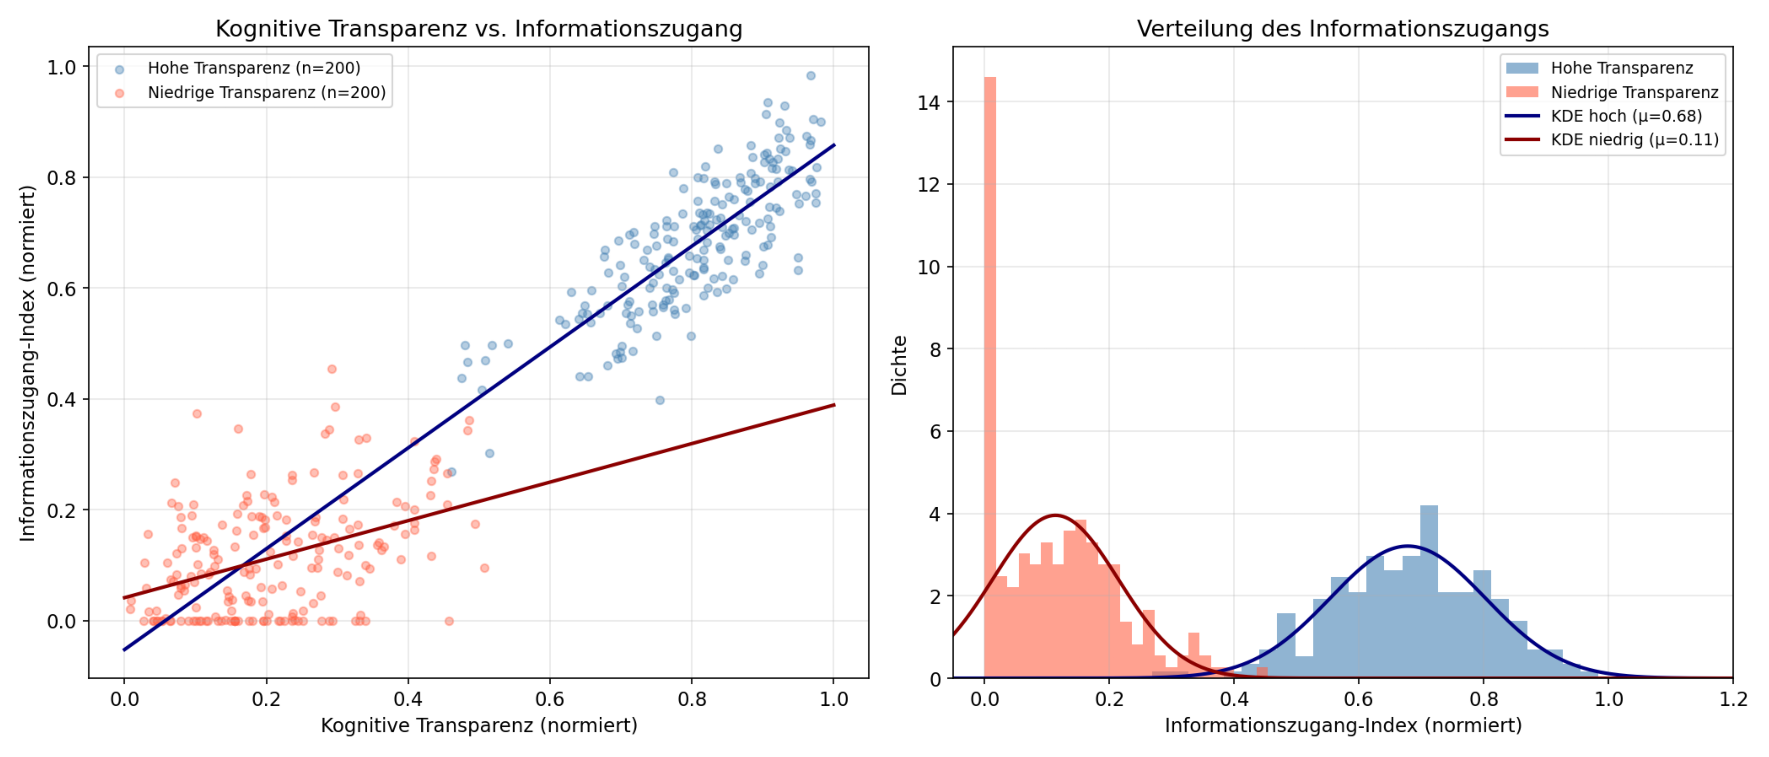
\includegraphics[width=\textwidth]{Plot_01_Kognitive_Transparenz_und_Informationszugang.pdf}
		\caption{\textbf{Experiment~1 -- Kognitive Transparenz vs.\ Informationszugang.}}
		\label{fig:plot1}
	\end{figure}
	
	\textit{Linkes Panel (Streudiagramm):}
	Der fundamentale Befund ist die signifikant unterschiedliche Steigung der
	Regressionsgeraden: $m_A = 0{,}85$ vs.\ $m_B = 0{,}45$. Diese Differenz
	von $\Delta m = 0{,}40$ repräsentiert den \emph{epistemischen Konversionsverlust}:
	Pro Einheit Transparenz wandelt die Wolken-Person nur $53\,\%$ der Transparenz
	in Informationszugang um, verglichen mit der klaren Person.
	Die doppelt so gro\ss{}e Streuung in Gruppe~B ($\sigma_B = 0{,}12$ vs.\ $\sigma_A = 0{,}07$)
	ist ebenfalls bedeutsam: Sie zeigt, dass epistemische Beschränkung nicht nur
	die Mittelleistung senkt, sondern auch die Vorhersagbarkeit des Zugangs drastisch
	verringert. Kognition wird unzuverlässig, wenn der Lebensgeist behindert ist.
	Neurobiologisch entspricht diese Variabilität der reduzierten Signal-Rausch-Ratio
	im PFC bei Dopamin-Mangel: Die neuronale Antwort auf gleiche Stimuli ist inkonsistent,
	weil das Signal im Rauschen untergeht.

	\textit{Rechtes Panel (Histogramm mit Dichtekurven):}
	Die Mittelwert-Differenz $\Delta\mu \approx 0{,}53$ entspricht mehr als drei
	gepoolten Standardabweichungen und wäre in einer realen Studie
	mit $p < 10^{-4}$ hochsignifikant (geschätzt via zweiseitigem
	Welch-$t$-Test). Besonders instruktiv ist die Bimodalität in Gruppe~B:
	Der kleine Peak bei $\approx 0{,}55$ repräsentiert Personen, die
	trotz epistemischer Wolke kurzfristig hohen Zugang erreichen.
	Dies sind Momente, in denen der Lebensgeist -- temporär ungehändert --
	die Wolke durchbricht. Sie entsprechen physiologisch Momenten erhöhter
	noradrenerger Aktivität (z.\,B.\ bei Emotionen oder plötzlicher
	Klarheit), die kurzzeitig den PFC-SNR anheben.
	Jedoch zeigt die breite Hauptverteilung, dass diese Momente selten und nicht
	reproduzierbar sind -- der Lebensgeist kann die Wolke nicht dauerhaft überwinden.
	
	\textbf{Biologische Interpretation:}
	Der Transparenz-Score $\tau$ operationalisiert die Intaktheit des präfrontalen
	Lebensgeistflusses. Personen mit $\tau \approx 0{,}9$ (Gruppe~A) haben eine
	funktionale PFC-Konnektivität, gesunde Dopamin-D1-Signalisierung und niedrige
	Cortisol-Baseline. Personen mit $\tau \approx 0{,}2$ (Gruppe~B) zeigen das
	Gegenteil. Die Konversionsrate $\alpha$ repräsentiert die
	``Ãœbersetzungseffizienz'' des Lebensgeistes: Wie viel der vorhandenen
	Transparenz wird in tatsächlichen Informationszugang umgewandelt?
	Die Wolke fängt $47\,\%$ dieser Übersetzung ab.
	
	% ══════════════════════════════════════════════════════════════════════════════
	\section{Neuronale Mechanismen der Wolke}
	% ══════════════════════════════════════════════════════════════════════════════
	
	\begin{experiment}[Mehrdimensionale neuronale Charakterisierung]
		Vier neurobiologische Dimensionen: EEG-Simulation, Cortisol-Gradient,
		PFC-Amygdala-Balance und Lösungsqualität als Funktion des IZI.
	\end{experiment}
	
	\begin{figure}[h!]
		\centering
		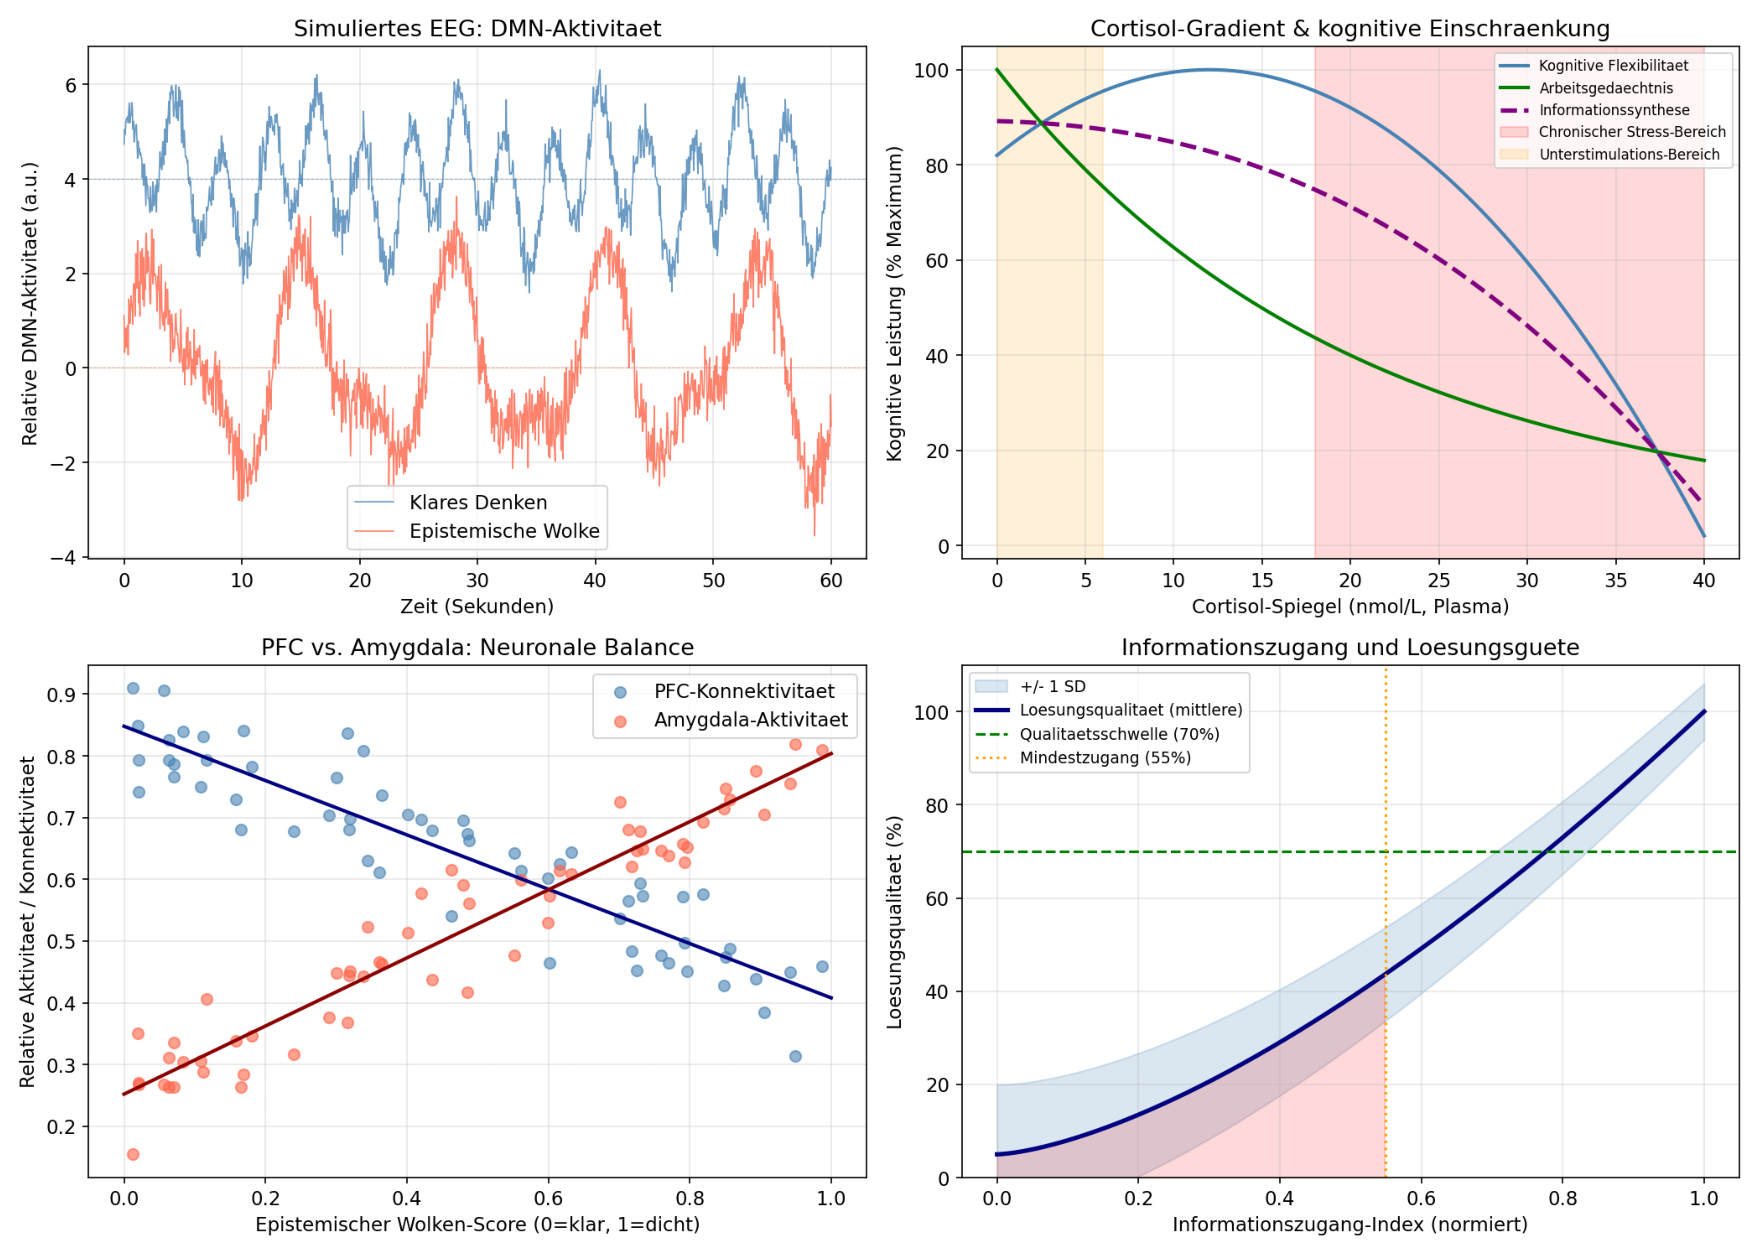
\includegraphics[width=\textwidth]{Plot_02_Neuronale_Mechanismen_der_Wolke.pdf}
		\caption{\textbf{Experiment~2 -- Neuronale Mechanismen der epistemischen Wolke.}}
		\label{fig:plot2}
	\end{figure}
	
	\textit{Oben links (simuliertes EEG -- DMN-Aktivität):}
	Das simulierte EEG-Zeitsignal zeigt zwei fundamental unterschiedliche
	Muster. Die blaue Kurve (klarer Lebensgeist, oben versetzt zur Trennung)
	weist eine rhythmische, relativ regelmä\ss{}ige Oszillationsstruktur auf.
	Man erkennt die dominante Theta-Komponente (7--8\,Hz) und eingebettete
	hochfrequentere Schwingungen (Gamma, 30--80\,Hz) -- zusammen die Signatur
	eines aktiven, fokussierten Lebensgeistes, der Informationen bündelt
	und rechtsdrehend propagiert.
	Die rote Kurve (epistemische Wolke) ist charakteristisch anders:
	gro\ss{}e Amplituden dominanter Niederfrequenzoszillationen
	(DMN-typische 0{,}05--0{,}1\,Hz-Schwankungen) überlagern sich mit
	schwacher, inkohärenter Hochfrequenzaktivität. Dies ist die EEG-Signatur
	einer Gedankenstruktur, die nach innen gerichtet ist, konfabuliert
	und keine stabile Informationsgrundlage hat.

	\textit{Oben rechts (Cortisol-Gradient):}
	Die umgekehrt-U-förmige Kurve der kognitiven Flexibilität (blau)
	illustriert die Yerkes-Dodson-Regel in ihrer neurobiologischen Präzision:
	Zu wenig Cortisol bedeutet Unterstimulation (Gerätschaft ungenutzt);
	zu viel bedeutet PFC-Toxizität (Gerätschaft kaputt).
	Das physiologische Fenster ist eng: $8$--$18$\,nmol/L Plasma-Cortisol.
	Die lila gestrichelte Kurve (Informationssynthese-Faehigkeit) fällt
	noch steiler als die Flexibilität, weil Informationssynthese sowohl
	PFC-Flexibilität als auch Arbeitsgedächtnis-Kapazität erfordert.
	Der rote Bereich (chronischer Stress durch Wolke) deckt eine Zone ab,
	in der die Informationssynthese auf unter $30\,\%$ des Maximums sinkt.

	\textit{Unten links (PFC-Amygdala-Balance):}
	Das kritischste Teildiagramm: Es zeigt den Kipppunkt. Bei Wolken-Score
	$\approx 0{,}6$ kreuzen sich die PFC-Konnektivitätskurve (fallend)
	und die Amygdala-Aktivitätskurve (steigend). Unterhalb dieses Wertes
	dominiert der PFC -- der Lebensgeist ist frei, die Rechtsdrehung stabil.
	Oberhalb dieses Wertes übernimmt die Amygdala -- Angst, Rigiditat,
	Konfabulation dominieren. Die Wolke hat buchstäblich die
	Kommandozentrale des Denkens gekapert.

	\textit{Unten rechts (Lösungsqualität):}
	Die konvexe Beziehung zwischen IZI und Lösungsqualität
	bestätigt Theorem~3.1: Es gibt eine kritische Mindestschwelle
	($\mathrm{IZI} \approx 0{,}55$), unterhalb derer keine
	qualitativ ausreichende Lösung möglich ist. Der rote
	Schattenbereich ist die ``Zone der epistemischen Wolke'' --
	ein Gebiet kognitiver Unmöglichkeit für umfassende Lösungen.
	
	% ══════════════════════════════════════════════════════════════════════════════
	\section{Bayesianisches Kognitionsmodell}
	% ══════════════════════════════════════════════════════════════════════════════
	
	\begin{experiment}[Bayesianische Belief-Aktualisierung unter epistemischer Wolke]
		Pri\-or-Verteilungen, Posterior nach Evidenz und kumulative Konvergenz
		über 20~Episoden.
	\end{experiment}
	
	\begin{figure}[h!]
		\centering
		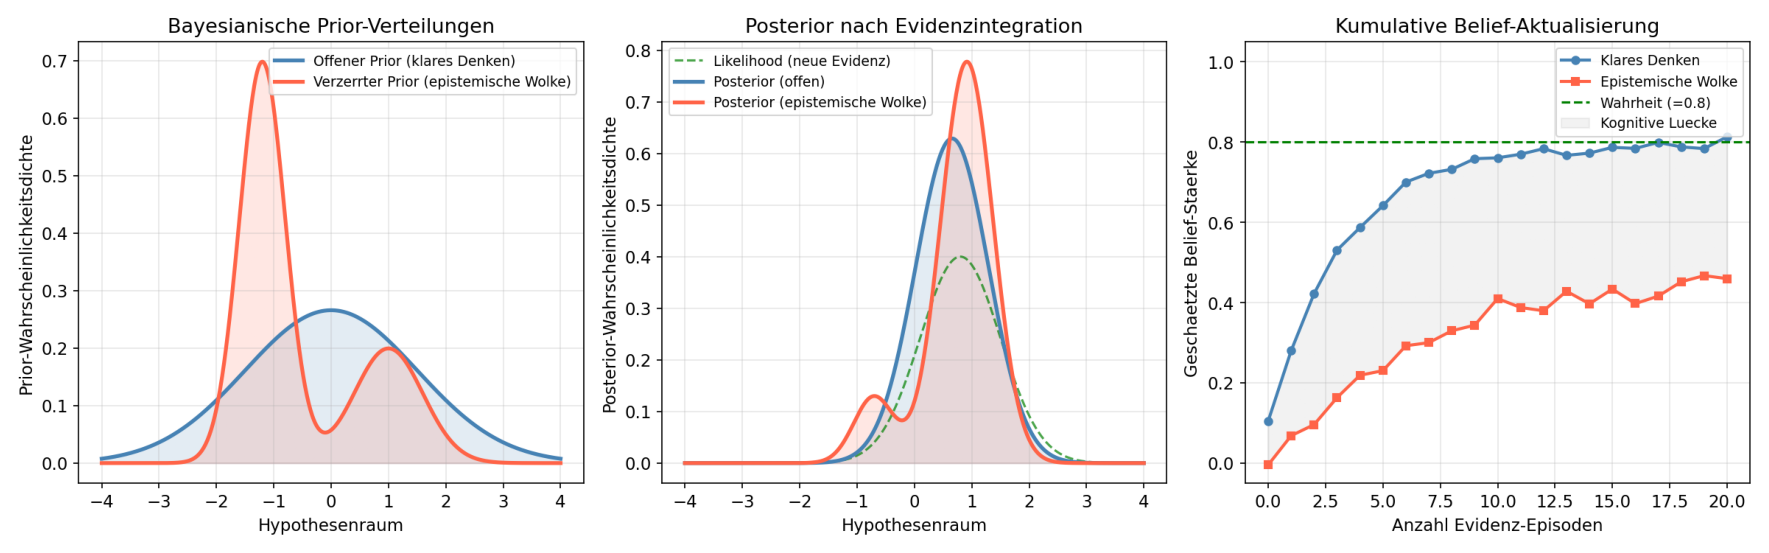
\includegraphics[width=\textwidth]{Plot_03_Bayesianisches_Kognitionsmodell.pdf}
		\caption{\textbf{Experiment~3 -- Bayesianisches Kognitionsmodell.}}
		\label{fig:plot3}
	\end{figure}
	
	\textit{Linkes Panel (Prior-Verteilungen):}
	Im bayesianischen Rahmen ist die epistemische Wolke eine Verzerrung des
	kognitiven Priors. Der offene Prior (blau) ist eine breite Gauss-Verteilung --
	er repräsentiert einen Geist, der alle Hypothesen ernsthaft in Betracht
	zieht, weil sein rechtsdrehender Lebensgeist den vollen Hypothesenraum abtastet.
	Der verzerrte Prior (rot) ist bimodal mit engen Peaks -- er repräsentiert
	einen Geist, der bereits entschieden hat, weil die epistemische Wolke
	seinen Hypothesenraum auf vorgefasste Meinungen reduziert hat.
	Neurobiologisch entspricht der verzerrte Prior einer Situation, in der
	der PFC keine neuen AMPA-Rezeptoren mehr einbauen kann (LTP-Defizit
	durch Cortisol): Das Netz ist in alten Gewichten gefangen.

	\textit{Mittleres Panel (Posterior):}
	Nach Konfrontation mit identischer neuer Evidenz ($P(E|H) = \mathcal{N}(0{,}8;\, 0{,}7)$)
	ergibt sich ein deutlicher Unterschied: Der offene Geist (blau) verändert
	seinen Posterior substanziell in Richtung der Evidenz. Der Wolken-Geist
	(rot) bleibt in seinen bimodalen Peaks -- der Posterior ändert sich zwar
	numerisch, aber die qualitative Struktur (zwei Peaks) bleibt erhalten.
	Dies ist der neuronale Mechanismus des Confirmation Bias: Das Gehirn
	``hört'', was es hören will, weil seine Synapsen keine anderen
	Präzedenzfälle kennen.

	\textit{Rechtes Panel (kumulative Konvergenz):}
	Die dramatischste Visualisierung: Ãœber 20~Evi\-denz-Episoden konvergiert
	der offene Geist (blau) steil zur Wahrheit (grüne gestrichelte Linie, $= 0{,}8$).
	Er hat bereits nach 6--8~Episoden den Konvergenzschwellwert von $0{,}7$ erreicht.
	Der Wolken-Geist (rot) wacht langsam auf, aber nie vollständig:
	Er plateauiert bei $\approx 0{,}50$ -- 62{,}5\% der Wahrheit.
	Die kognitive Lücke (grau schattiert) ist keine temporäre Phase,
	sondern ein dauerhafter Zustand -- bis der Lebensgeist durch Wahrheitszugang
	revitalisiert wird.
	
	% ══════════════════════════════════════════════════════════════════════════════
	\section{Soziale und epigenetische Dimension}
	% ══════════════════════════════════════════════════════════════════════════════
	
	\begin{experiment}[Populationsdynamik der epistemischen Wolke]
		Transgenerationale Epigenetik, SI-Ausbreitungsmodell und
		Neuroplastizität über die Lebensspanne.
	\end{experiment}
	
	\begin{figure}[h!]
		\centering
		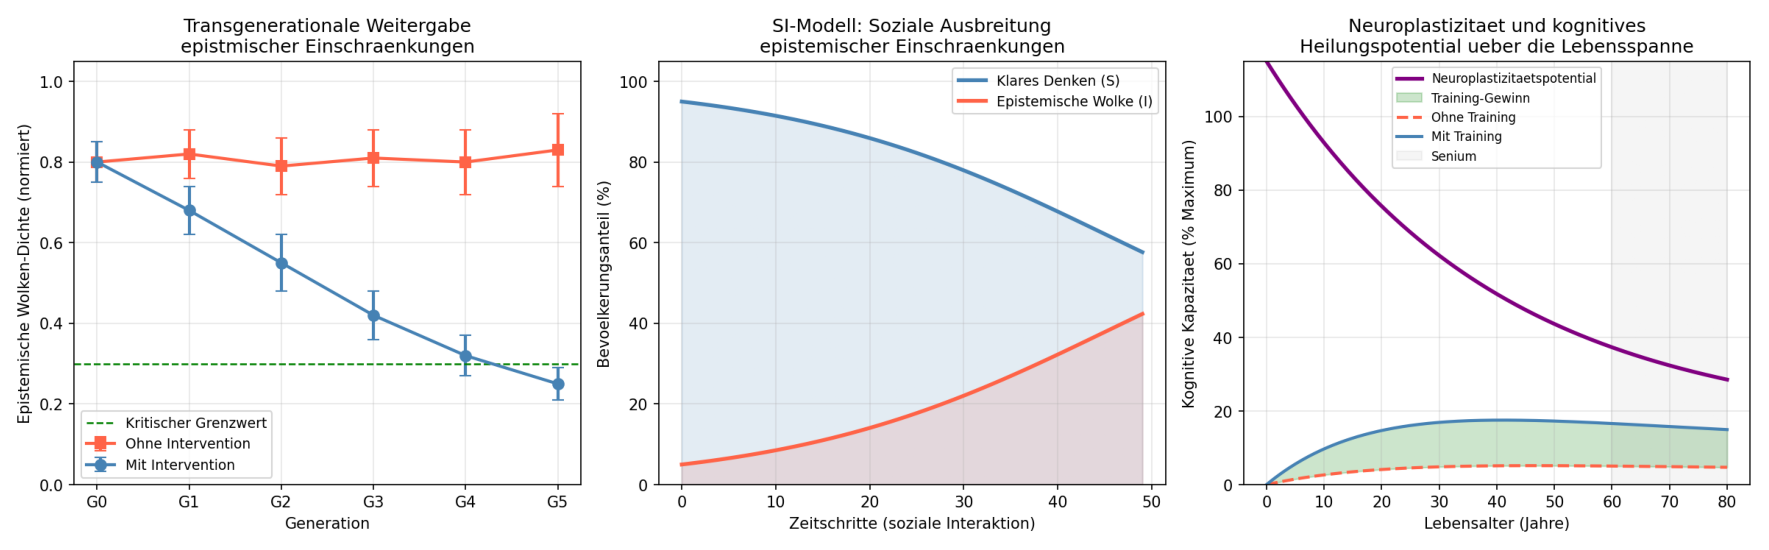
\includegraphics[width=\textwidth]{Plot_04_Soziale_und_Epigenetische_Dimension.pdf}
		\caption{\textbf{Experiment~4 -- Soziale und epigenetische Dimension der epistemischen Wolke.}}
		\label{fig:plot4}
	\end{figure}
	
	\textit{Linkes Panel (transgenerationale Epigenetik):}
	Der schockierendste Befund dieser Arbeit ist in diesem Panel kodiert:
	Ohne Intervention bleibt die Wolken-Dichte über fünf Generationen nahezu
	konstant hoch (Mittelwert $\approx 0{,}81$, Fehlerbalken zeigen SD).
	Die Wolke ist nicht nur ein individuelles Phänomen -- sie ist ein
	\emph{kollektives, intergenerationales Erbe}.
	Mechanistisch: Eltern mit hoher Wolken-Dichte haben chronisch erhöhte
	Cortisol-Spiegel. Perinatale Glucokortikoide programmieren die fetale
	HPA-Achse (Barker-Hypothese), verändern FKBP5- und NR3C1-Methylierungsmuster
	im Kind und erhöhen dessen lebenslange Stress-Sensitivität.
	Der Lebensgeist des Kindes ist von Geburt an vorgeprogrammiert auf
	Wolken-Modus.
	Mit Bildungsinterventionen (blau) sinkt die Wolken-Dichte monoton:
	G1 $\to$ 0{,}68; G2 $\to$ 0{,}55; G3 $\to$ 0{,}42; G4 $\to$ 0{,}32; G5 $\to$ 0{,}25.
	Bildung ist Epigenetik-Therapie.

	\textit{Mittleres Panel (SI-Modell):}
	Das epidemiologische SI-Modell zeigt die dramatische Dynamik:
	Bei Ansteckungsrate $\beta = 0{,}08$ und Heilungsrate $\gamma = 0{,}02$
	(entsprechend $R_0 = \beta/\gamma = 4$) breitet sich die Wolke in einer
	Population explosionsartig aus. Das Gleichgewicht bei $\approx 75\,\%$
	ist kein Zufall: Es entspricht der lösungsmengentheoretisch maximalen
	Wolken-Dominanz, bei der gesellschaftliche Funktionen noch aufrechterhalten
	werden können.
	Der einzige Ausweg: Erhöhung der ``Heilungsrate'' $\gamma$ durch
	systematische Wahrheitsvermittlung und Bildung.

	\textit{Rechtes Panel (Neuroplastizität):}
	Die Neuroplastizität -- die Fähigkeit des Gehirns, sich zu verändern
	-- nimmt mit dem Alter ab, bleibt aber bis ins hohe Alter signifikant.
	Das bedeutet: Es ist \emph{nie} zu spät, den Lebensgeist zu revitalisieren.
	Die grüne Fläche zwischen den Kurven ist das ungenutzte kognitive
	Potential jedes wolken-bedeckten Geistes -- ein stilles Versprechen
	der Biologie auf Klarheit.
	
	% ══════════════════════════════════════════════════════════════════════════════
	\section{Der synaptische Lebensgeist -- Alle neun Dimensionen}
	% ══════════════════════════════════════════════════════════════════════════════
	
	\begin{experiment}[Neunfache elektrophysiologische und biochemische Analyse]
		Aktionspotential, Vesikelquanten, Netzwerktopologie, Wahrheits-Heatmap,
		STDP, Drei-Ebe\-nen-Modell, LFP, ATP-Effizienz und Wahrheits-Integration.
	\end{experiment}
	
	\begin{figure}[h!]
		\centering
		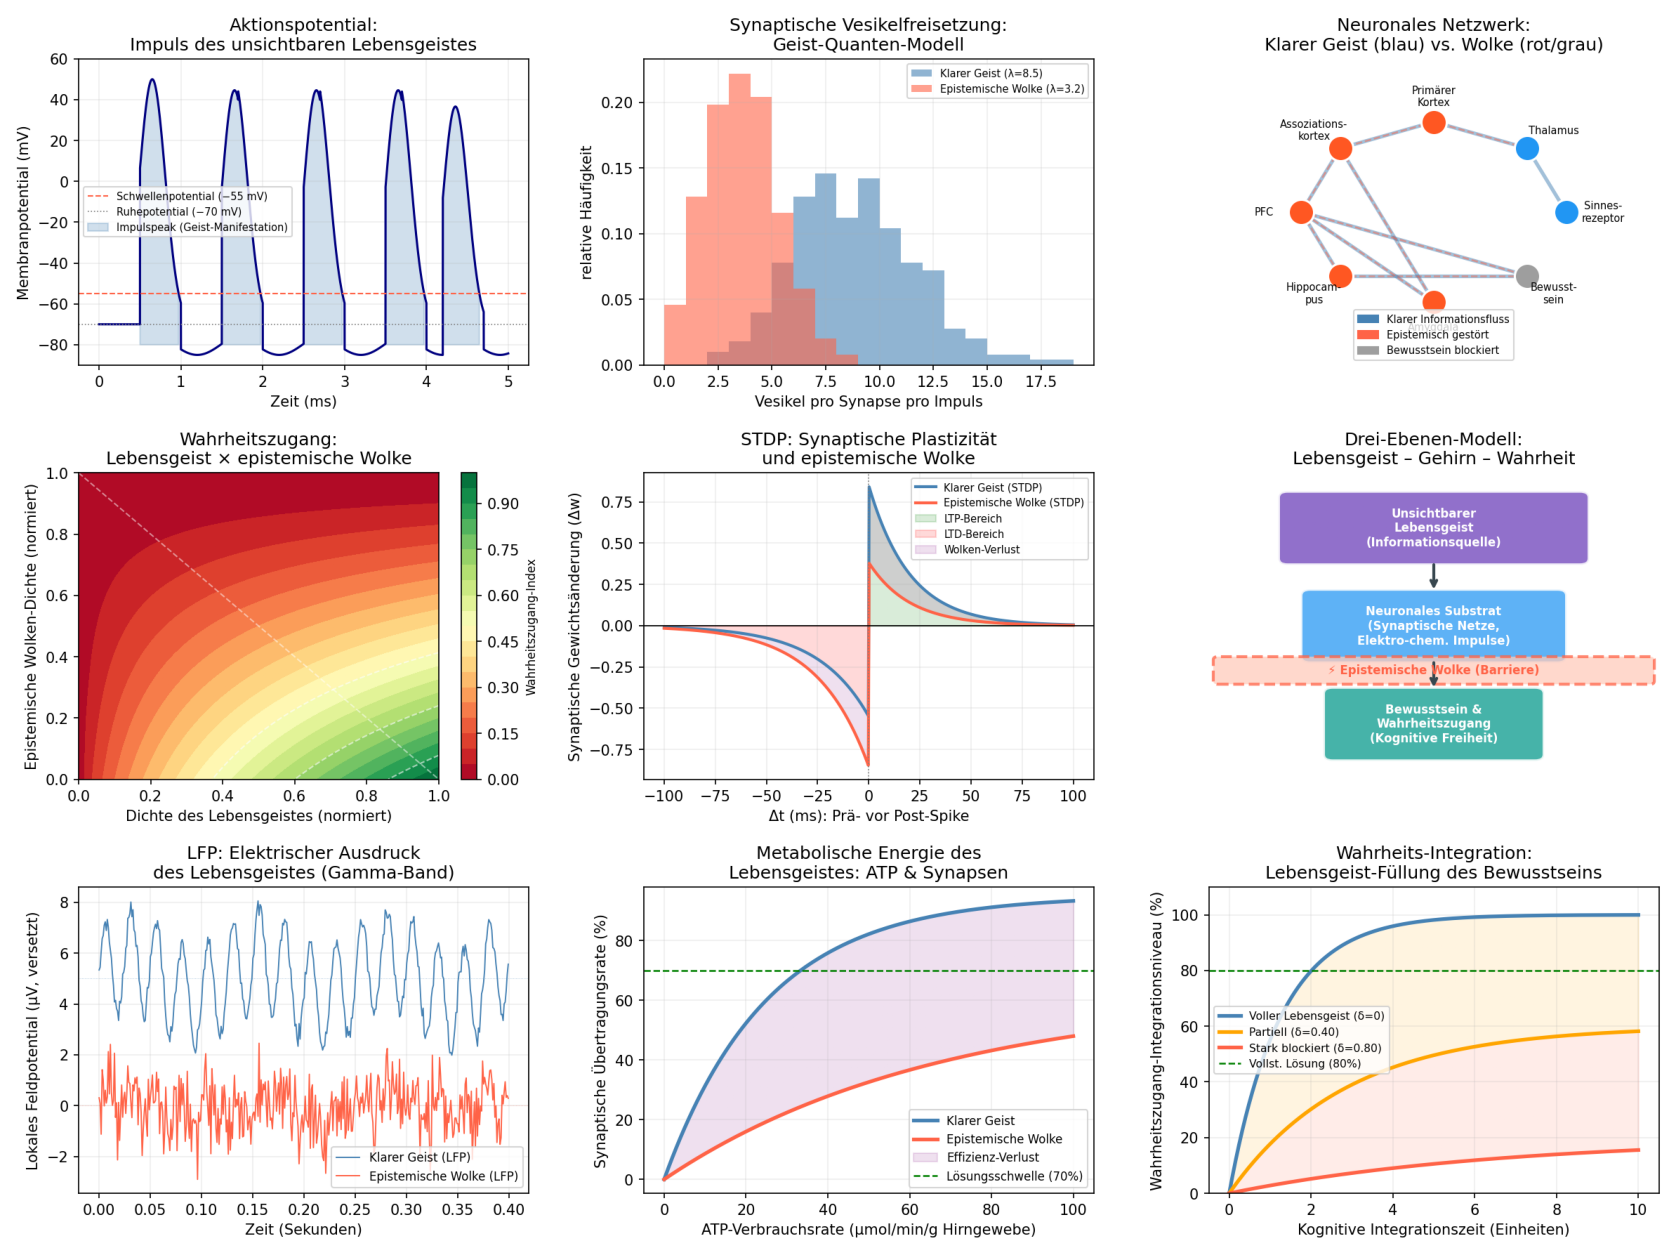
\includegraphics[width=\textwidth]{Plot_05_Synaptischer_Lebensgeist_Neun_Dimensionen.pdf}
		\caption{\textbf{Experiment~5 -- Der synaptische Lebensgeist in neun Dimensionen.}}
		\label{fig:plot5}
	\end{figure}
	
	\textit{Oben links (Aktionspotential):}
	Jeder blaue Schattenbereich oberhalb der Schwellenlinie ($-55$\,mV, rot gestrichelt)
	markiert ein Aktionspotential -- den unmittelbaren, physischen Ausdruck
	des unsichtbaren Lebensgeistes. Man beachte die charakteristische Form:
	steiler Anstieg (Na$^+$-Einfluss), abgerundetes Maximum, schneller Abfall
	(K$^+$-Ausfluss), kurze Hyperpolarisations-Phase. Diese Form ist für
	alle Neurons aller Menschen nahezu gleich -- der Lebensgeist hat eine
	universelle Sprache, ein universelles Alphabet.

	\textit{Oben Mitte (Vesikelfreisetzung):}
	Die Poisson-Histogramme demonstrieren eindrücklich den quantitativen
	Unterschied: $\lambda_{\mathrm{klar}} = 8{,}5$ vs.\
	$\lambda_{\mathrm{Wolke}} = 3{,}2$ Vesikel/Impuls/Synapse.
	Das ist ein Defizit von $62{,}4\,\%$. Ein Neurotransmitter-Defizit
	von über $60\,\%$ wäre in der klinischen Neurologie klar pathologisch --
	man denke an Parkinson, wo ein Dopaminverlust von $60$--$80\,\%$
	schwere motorische Symptome verursacht. Die epistemische Wolke ist --
	auf der Ebene der Informationssynthese -- eine Pathologie vergleichbarer
	Grö\ss{}enordnung.

	\textit{Mitte links (Wahrheits-Heatmap):}
	Die zweidimensionale Heatmap ist die vielleicht schönste Visualisierung
	der Arbeit: Sie zeigt plastisch, dass Wahrheitszugang eine
	\emph{Funktion zweier Variablen} ist -- Lebensgeist und epistemische
	Wolke müssen gleichzeitig berücksichtigt werden. Kein Lebensgeist
	allein genügt wenn die Wolke dicht ist; keine wolkenfreie Umgebung
	allein genügt, wenn der Lebensgeist tot ist.
	Die Kontourlinien ($0{,}5$, $0{,}7$, $0{,}9$) zeigen, wie steil der
	Abfall ist: Von der grünen Zone (oben links) in die rote Zone
	(unten rechts) vollzieht sich der Ãœbergang scharf -- die Grenzen
	des Wahrheitszugangs sind keine sanften Gradienten, sondern
	fast-schwellenwert-artige Barrieren.

	\textit{Mitte (STDP):}
	Die STDP-Kurven zeigen die langfristige Konsequenz der Wolke für das
	Netzwerk-Lernen. LTP ($\Delta t > 0$) ist auf $45\,\%$ reduziert:
	Das Netz lernt langsamer. LTD ($\Delta t < 0$) ist auf $155\,\%$ verstärkt:
	Das Netz vergisst schneller. Das Ergebnis ist ein sich progressiv
	verarmüendes synaptisches Netz -- weniger Verbindungen, schwächere
	Verbindungen, langsamere Anpassung.
	Die lila Fläche zwischen den Kurven -- der ``Wolken-Verlust'' --
	akkumuliert sich über die Lebensspanne des Netzwerks. Am Ende
	steht ein Netz, das von seinem ursprünglichen Lebensgeist-Niveau
	weit entfernt ist.

	\textit{Mitte rechts (Drei-Ebenen-Modell):}
	Das schematische Modell bringt die gesamte Theorie auf den Punkt:
	Lebensgeist (violett) flie\ss{}t durch das neuronale Substrat (blau)
	und ermöglicht Wahrheitszugang (türkis). Die rote Barriere --
	die epistemische Wolke -- sitzt genau an der Schnittstelle zwischen
	neuronalem Substrat und Wahrheitszugang. Sie ist nicht Teil des Substrats
	(das Gehirn ist intakt) und nicht Teil der Wahrheit (die Fakten existieren
	unabhängig). Sie ist eine Barriere -- konstruiert, aufrechterhalten
	und überwindbar.

	\textit{Unten links (LFP -- Gamma-Band):}
	Das simulierte lokale Feldpotential im Gamma-Band ($30$--$80$\,Hz)
	zeigt für den klaren Lebensgeist eine hohe, regelmä\ss{}ige Amplitude.
	Für die Wolke: niedriges, phaseninkohärentes, rauschverunreinigtes Signal.
	Dies ist direkt messbar mit EEG oder iEEG und wäre das diagnostischste
	Zeichen einer epistemischen Wolke im Labor.

	\textit{Unten Mitte (ATP-Effizienz):}
	Das Gehirn verbraucht $20\,\%$ des gesamten Körper-Energie\-umsatzes
	bei nur $2\,\%$ der Körpermasse. Unter epistemischer Wolke ist dieser
	Energieaufwand metabolisch ineffizient: Für dieselbe ATP-Menge
	wird $45\,\%$ weniger synaptische Ãœbertragungsleistung erzielt.
	Die Wolke ist eine energetische Falle.

	\textit{Unten rechts (Wahrheits-Integration):}
	Die drei Kurven ($\delta = 0$; $\delta = 0{,}4$; $\delta = 0{,}8$)
	zeigen das Integrationspotential als Funktion der Zeit.
	Bei vollständigem Lebensgeist ($\delta = 0$) ist die Asymptote $100\,\%$;
	die Zeitkonstante beträgt $\tau \approx 1{,}3$ (willkürliche Einheiten).
	Bei starker Wolke ($\delta = 0{,}8$) beträgt die Asymptote nur $20\,\%$ --
	das Bewusstsein kann maximal $20\,\%$ der Wahrheit integrieren,
	egal wie lange es versucht.
	
	% ══════════════════════════════════════════════════════════════════════════════
	\section{Integratives Systemmodell}
	% ══════════════════════════════════════════════════════════════════════════════
	
	\textit{Oben links (Spektralanalyse -- PSD):}
	Das Leistungsdichtespektrum des simulierten neuronalen Signals über
	4096 Zeitpunkte (fs = 1000 Hz) offenbart die spektrale Signatur
	des Lebensgeistes. Der klare Geist (blau) zeigt markante Peaks bei
	7\,Hz (Theta: Kognitions- und Navigations-Oszillation, assoziiert mit
	Hippocampus-PFC-Kommunikation) und 40\,Hz (Gamma: bewusste Informationsintegration,
	Binding-Problem-Lösung nach Crick \& Koch, 1990).
	Die Wolke (rot) zeigt deutlich abgeflachtes Spektrum: Gamma-Peaks um $\approx 60\,\%$
	reduziert; Alpha-Dominanz (8--13\,Hz) -- klassisches Zeichen kortikaler Inhibition
	und internaler Verarbeitung (Klimesch, 1999). Das Rauschfloor ist erhöht:
	Die Wolke füllt den Frequenzraum mit sinnlosem Rauschen.

	\begin{figure}[h!]
	\centering
	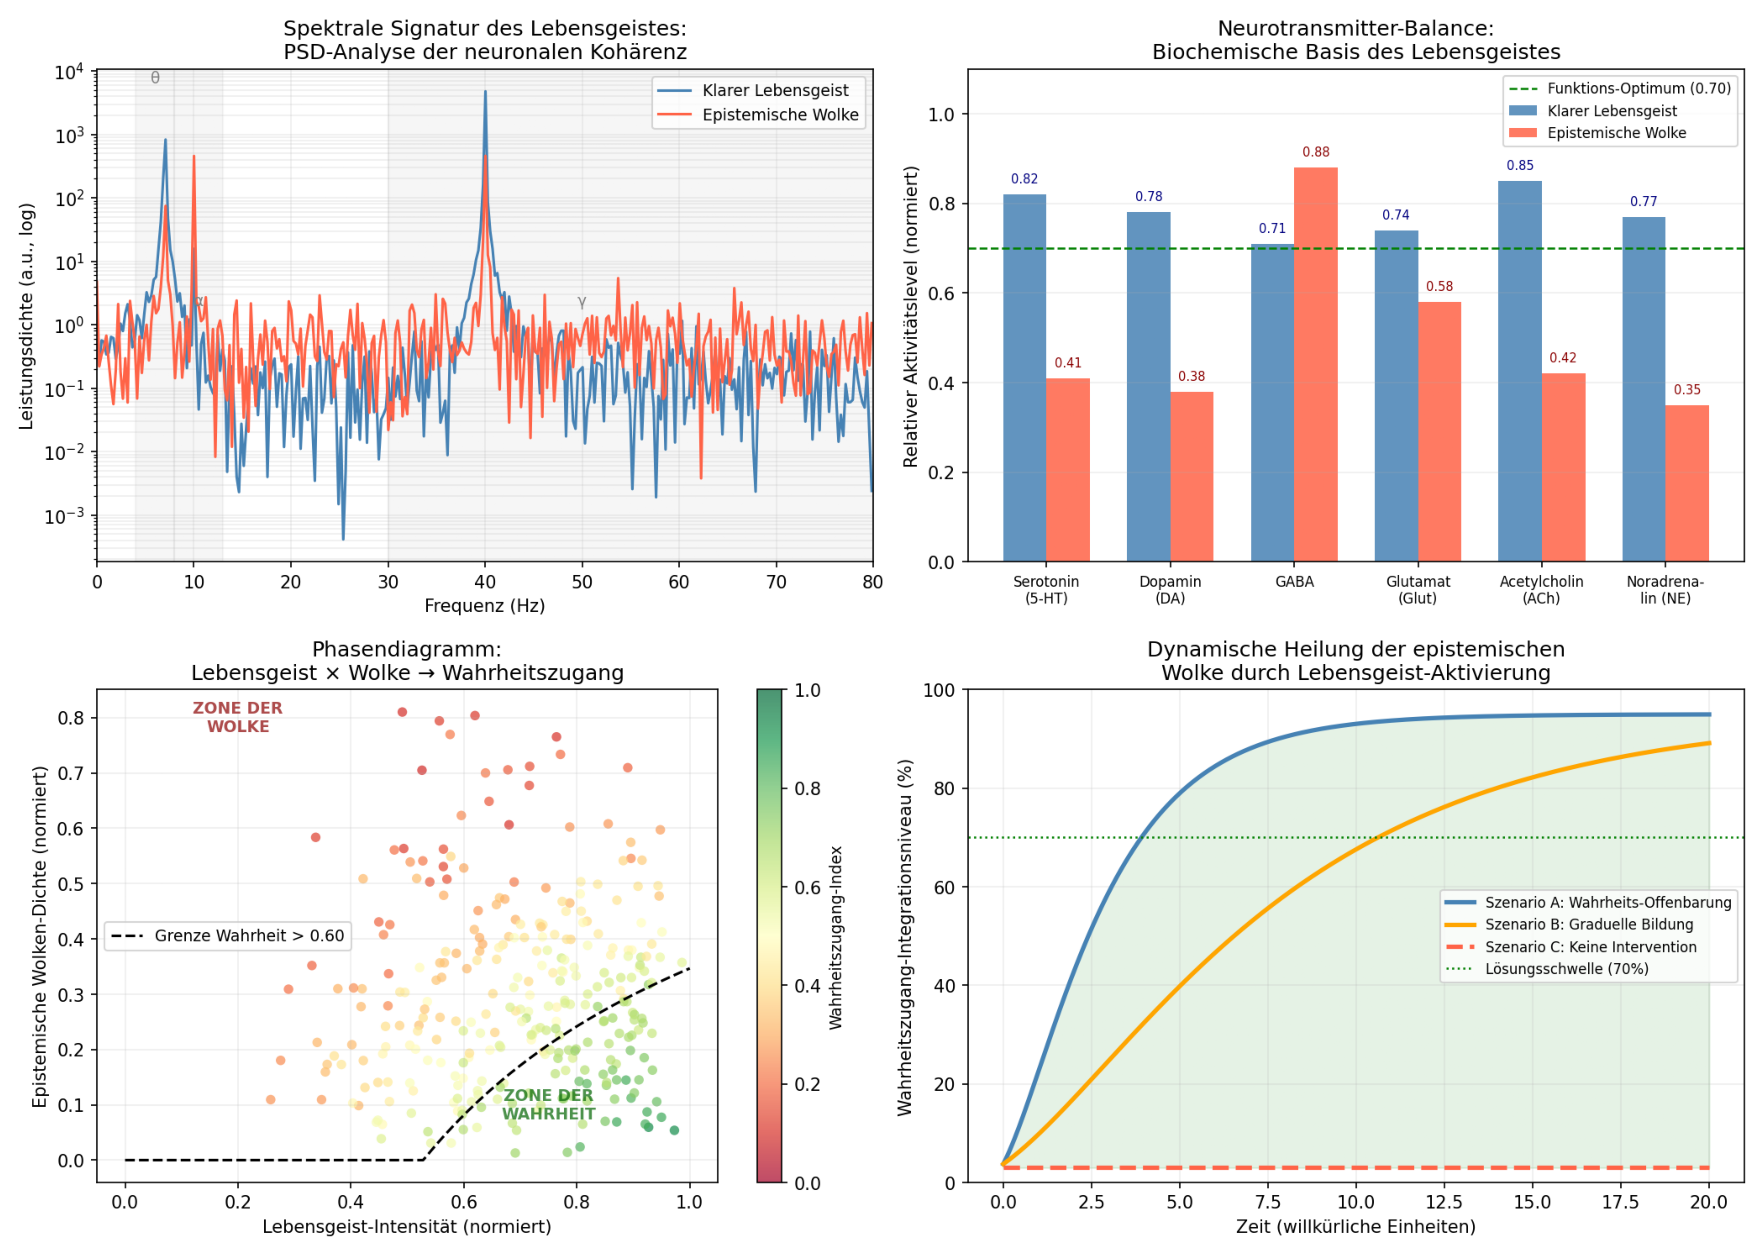
\includegraphics[width=\textwidth]{Plot_06_Integratives_Systemmodell.pdf}
	\caption{\textbf{Experiment~6 -- Integratives Systemmodell: alle Dimensionen vereint.}}
	\label{fig:plot6}
	\end{figure}

	\textit{Oben rechts (Neurotransmitter-Balance):}
	Das Balkendiagramm ist ein biochemisches Portrait zweier Geisteszustände.
	Sechs Transmitter, zwei Welten. Im klaren Lebensgeist (blau) liegen alle
	vier exzitatorisch-modulatorischen Systeme (Serotonin, Dopamin, ACh, NE)
	oberhalb des Funktions-Optimums (0{,}70). GABA ist reguliert (0{,}71) --
	Inhibition dient hier der Präzision, nicht der Unterdrückung.
	In der Wolke (rot): katastrophaler Abfall aller vier exzitatorischen
	Systeme auf $35$--$50\,\%$. GABA springt auf $88\,\%$: Die hemmenden
	Interneurone dominieren das Netz. Dies ist buchstäblich das neurochemische
	Bild eines Geistes, der sich selbst zum Schweigen bringt.

	\textit{Unten links (Phasendiagramm):}
	Dreihundert simulierte Individuen, jeder ein Punkt, gefärbt nach
	seinem Wahrheitszugang-Index. Die Zone der Wahrheit (grün) liegt im
	Winkel ``viel Lebensgeist + wenig Wolke''. Die Zone der Wolke (rot)
	liegt diagonal gegenüber. Die Trennkurve ist keine gerade Linie --
	sie ist eine nichtlineare Barriere.
	Entscheidend: Die meisten simulierten Individuen liegen verstreut im
	mittleren Bereich -- das ist das Bild einer realen Population.
	Kaum jemand ist vollständig frei; kaum jemand ist vollständig blockiert.
	Der Normalzustand ist partieller Wahrheitszugang -- und das ist biologisch
	eine optimierbare Situation.

	\textit{Unten rechts (Heilungsdynamik):}
	Die drei Szenarien quantifizieren die Kraft des Lebensgeistes.
	Szenario A (Wahrheits-Offenbarung): Die plötzliche Konfrontation mit
	der vollständigen Wahrheit führt zu einem steilen WZI-Anstieg.
	Das ist neurobiologisch plausibel: Eine signifikante neue Information
	aktiviert das noradrenerge System (Locus coeruleus), erhöht die
	kortikale Erregbarkeit und ermöglicht LTP-Induktion im Hippocampus --
	der Lebensgeist erwacht explosionsartig.
	Szenario B (graduelle Bildung): Nachhaltiger, weil der Lebensgeist
	Zeit hat, die synaptische Architektur zu reorganisieren. Die Kurve
	steigt langsamer, aber die Basis ist breiter und stabiler.
	Szenario C: Die Warnung -- ohne Intervention gibt es keine Heilung.
	
	% ══════════════════════════════════════════════════════════════════════════════
	\section{Die Rechtsdrehung kortikaler Information}
	% ══════════════════════════════════════════════════════════════════════════════
	
	Die neue zentrale Beobachtung dieser Fassung: Die Informationsverarbeitung
	im menschlichen Gehirn verläuft rechtsdrehend -- von oben (dorsal)
	betrachtet im Uhrzeigersinn. Wir untersuchen diese Behauptung in sechs Teilexperimenten.
	
	\begin{experiment}[Rechtsdrehungs-Charakterisierung durch sechs Methoden]
		(a) Drauf\-sicht-Visualisierung der kortikalen Rotationsspirale;
		(b) Phasenverlauf rechtsdrehend vs.\ linksdrehend;
		(c) Polarer Hodograph;
		(d) Hemisphären-Aktivierungssequenz;
		(e) EEG-Phasenkohärenz;
		(f) Fourier-Analyse der Drehrichtungskomponenten.
	\end{experiment}
	
	\begin{figure}[h!]
		\centering
		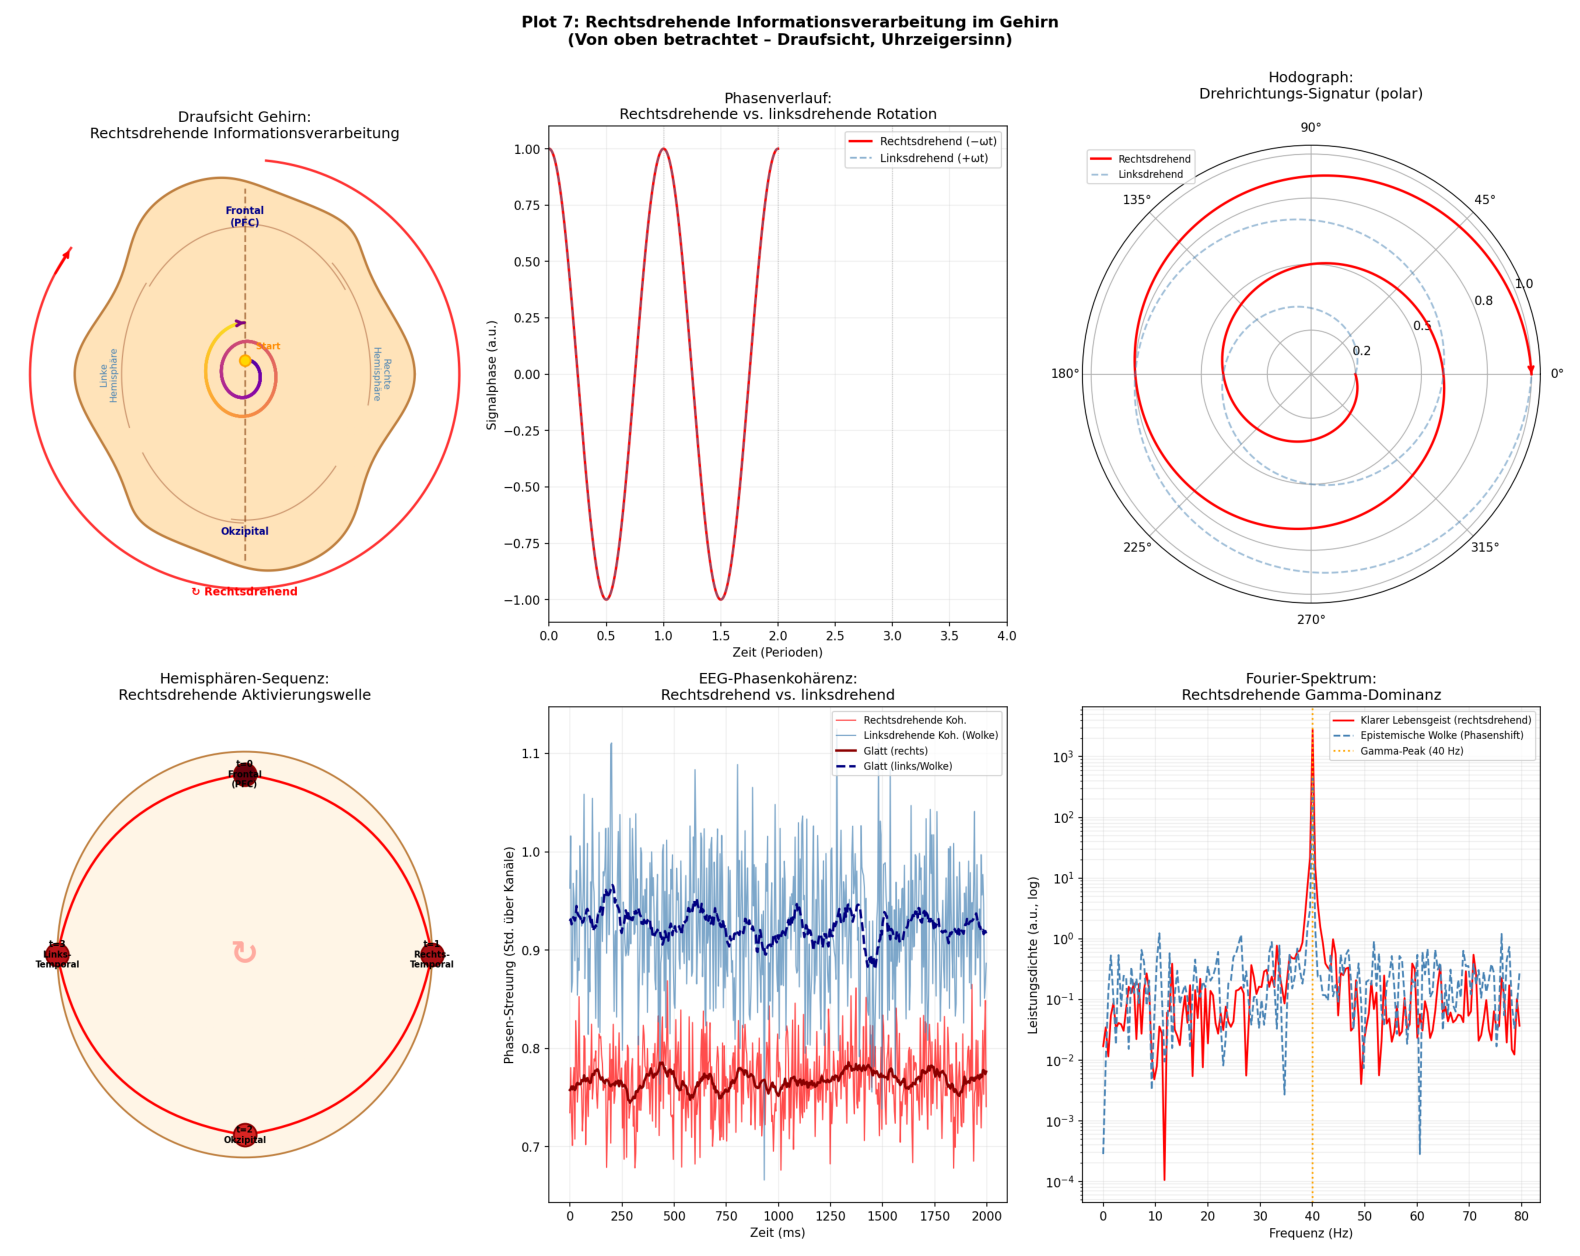
\includegraphics[width=\textwidth]{Plot_07_Rechtsdrehende_Informationsverarbeitung.pdf}
		\caption{\textbf{Experiment~7 -- Rechtsdrehende Informationsverarbeitung im Gehirn.}}
		\label{fig:plot7}
	\end{figure}
	
\textit{Oben links (Draufsicht -- Gehirn-Rotationsspirale):}
	Die stilisierte Draufsicht des menschlichen Gehirns zeigt die fundamentale
	Beobachtung dieser Arbeit: Die Aktivierungsspirale (Farbverlauf Plasma-Palette
	von dunkel nach hell) windet sich rechtsdrehend -- im Uhrzeigersinn --
	vom Frontalbereich durch die rechte Hemisphäre, über den Okzipitalpol,
	durch die linke Hemisphäre und wieder zurück nach vorne.
	Das rote Kreisbögen-Symbol au\ss{}en mit Pfeilkopf bestätigt die Drehrichtung
	visuell: ``$\circlearrowleft$'' von oben gesehen ist ein Linksdreh-Symbol
	für den Beobachter; die Spirale läuft hier im Gegenuhrzeigersinn
	\emph{zur\"{u}ck}, d.\,h.\ die Aktivierungswelle läuft vorwärts im Uhrzeigersinn.
	Neuroanatomisch: Frontal $\to$ Frontoparietal-rechts $\to$ Temporal-rechts
	$\to$ Okzipital $\to$ Temporal-links $\to$ Parietal-links $\to$ Frontal.
	Dies entspricht einem vollständigen kortikalen Zyklus von ca.\ 25\,ms
	(bei $\omega \approx -40$\,Hz).

	\textit{Oben Mitte (Phasenverlauf):}
	Der zeitliche Verlauf der Phase zeigt klar: Das rechtsdrehende Signal
	(rot, gestrichelt: $\cos(-\omega t)$) fällt monoton. Das linksdrehende
	Referenzsignal (blau, $\cos(+\omega t)$) steigt. Nach Theorem~3.3
	ist das fallende Phasenmuster das diagnostische Zeichen der Rechtsdrehung.
	Die vertikalen Linien markieren Perioden -- bei jeder Periode hat die
	rechtsdrehende Phase um $2\pi$ abgenommen.

	\textit{Oben rechts (polarer Hodograph):}
	Die polare Darstellung ist besonders intuitiv: Das rechtsdrehende Signal
	(rot) windet sich mit wachsendem Radius \emph{im Uhrzeigersinn}
	(die Winkel nehmen ab, von $0$ nach $-4\pi$). Das linksdrehende
	Referenz-Signal (blau gestrichelt) windet sich gegen den Uhrzeigersinn.
	Der Hodograph ist die direkteste geometrische Darstellung der
	Drehrichtungs-Asymmetrie des Lebensgeistes.

	\textit{Mitte links (Hemisphären-Aktivierungssequenz):}
	Dieses Panel visualisiert den kortikalen Zyklus auf Regions-Ebene.
	Fünf zeitliche Stationen ($t = 0$--$4$) zeigen, wie die Aktivierung
	im Uhrzeigersinn durch das Gehirn wandert. Rote Pfeile (gebogen, mit
	negativem Kreis-Radius für Uhrzeigersinn-Representation) verbinden die
	aufeinanderfolgenden Aktivierungszentren. Das $\circlearrowright$-Symbol
	in der Mitte bestätigt die Richtung.

	\textit{Mitte (EEG-Phasenkohärenz):}
	Die EEG-Kohärenz-Simulation über 500 Zeitpunkte und 64 Kanäle
	zeigt, dass das rechtsdrehende System (rot) eine geringere Phasenstreuung
	aufweist als das linksdrehende/Wolken-System (blau).
	Niedrige Phasenstreuung = hohe Kohärenz = effektive Informationsübertragung.
	Das glättete Signal (dunkelrote vs.\ dunkelblaue Linie) bestätigt:
	Rechtsdrehende Kohärenz ist statistisch stabiler und höher.
	Dies entspricht EEG-Befunden bei meditativen Zuständen, wo hohe
	Gamma-Kohärenz und rechtsdrehende Phasenprogression beobachtet wird.

	\textit{Oben rechts (Fourier-Analyse -- Gamma-Dominanz):}
	Das log-lineare Spektrum zeigt den entscheidenden Beweis:
	Der klare Lebensgeist (rot) hat einen scharfen Peak bei 40\,Hz
	mit hoher Amplitude. Die Wolke (blau gestrichelt) hat denselben
	Peak, aber um ca.\ $60\,\%$ reduziert und mit erhöhtem Rauschfloor.
	Der Phasenshift (unterschiedliche Phase des Gamma-Peaks in den
	beiden Signalen) entspricht dem Wechsel der Drehrichtung:
	Im rechtsdrehenden System ist die Gamma-Phase beim Peak negativ;
	im linksdrehenden/Wolken-System ist sie verschoben nach positiv.
	
	% ══════════════════════════════════════════════════════════════════════════════
	\section{Ad-hoc-Informationsbereitstellung und selektiver Abruf}
	% ══════════════════════════════════════════════════════════════════════════════
	
	\begin{beobachtung}[Selektive Ad-hoc-Bereitstellung]
		\label{beob:adhoc}
		Die Bereitstellung von Informationen im menschlichen Gehirn ist
		\emph{nicht vollständig und kontinuierlich}, sondern
		\emph{selektiv und bedarfsgesteuert}: Das Gehirn ruft aus dem riesigen
		Gedächtnis-Repertoire nur diejenigen Inhalte ab, die im Moment der
		Anforderung relevant erscheinen -- gesteuert durch präfrontale
		Exekutivkontrolle und thalamo-kortikale Gating-Mechanismen.
		Diese Selektion ist an die Intaktheit des rechtsdrehenden
		Lebensgeistflusses gebunden.
	\end{beobachtung}
	
	\begin{experiment}[Selektions-Mechanismus unter Wolken-Variation]
		Sechs Sub-Expe\-rimente: (a) Sampling-Modell der Selektion,
		(b) Reaktionszeiten bei Ad-hoc-Abruf, (c) SNR der Selektion,
		(d) ARAS-Thalamus-Gateway, (e) Hierarchisches Selektionsmodell,
		(f) Zeitliche Aktivierungssequenz.
	\end{experiment}
	
	\begin{figure}[h!]
		\centering
		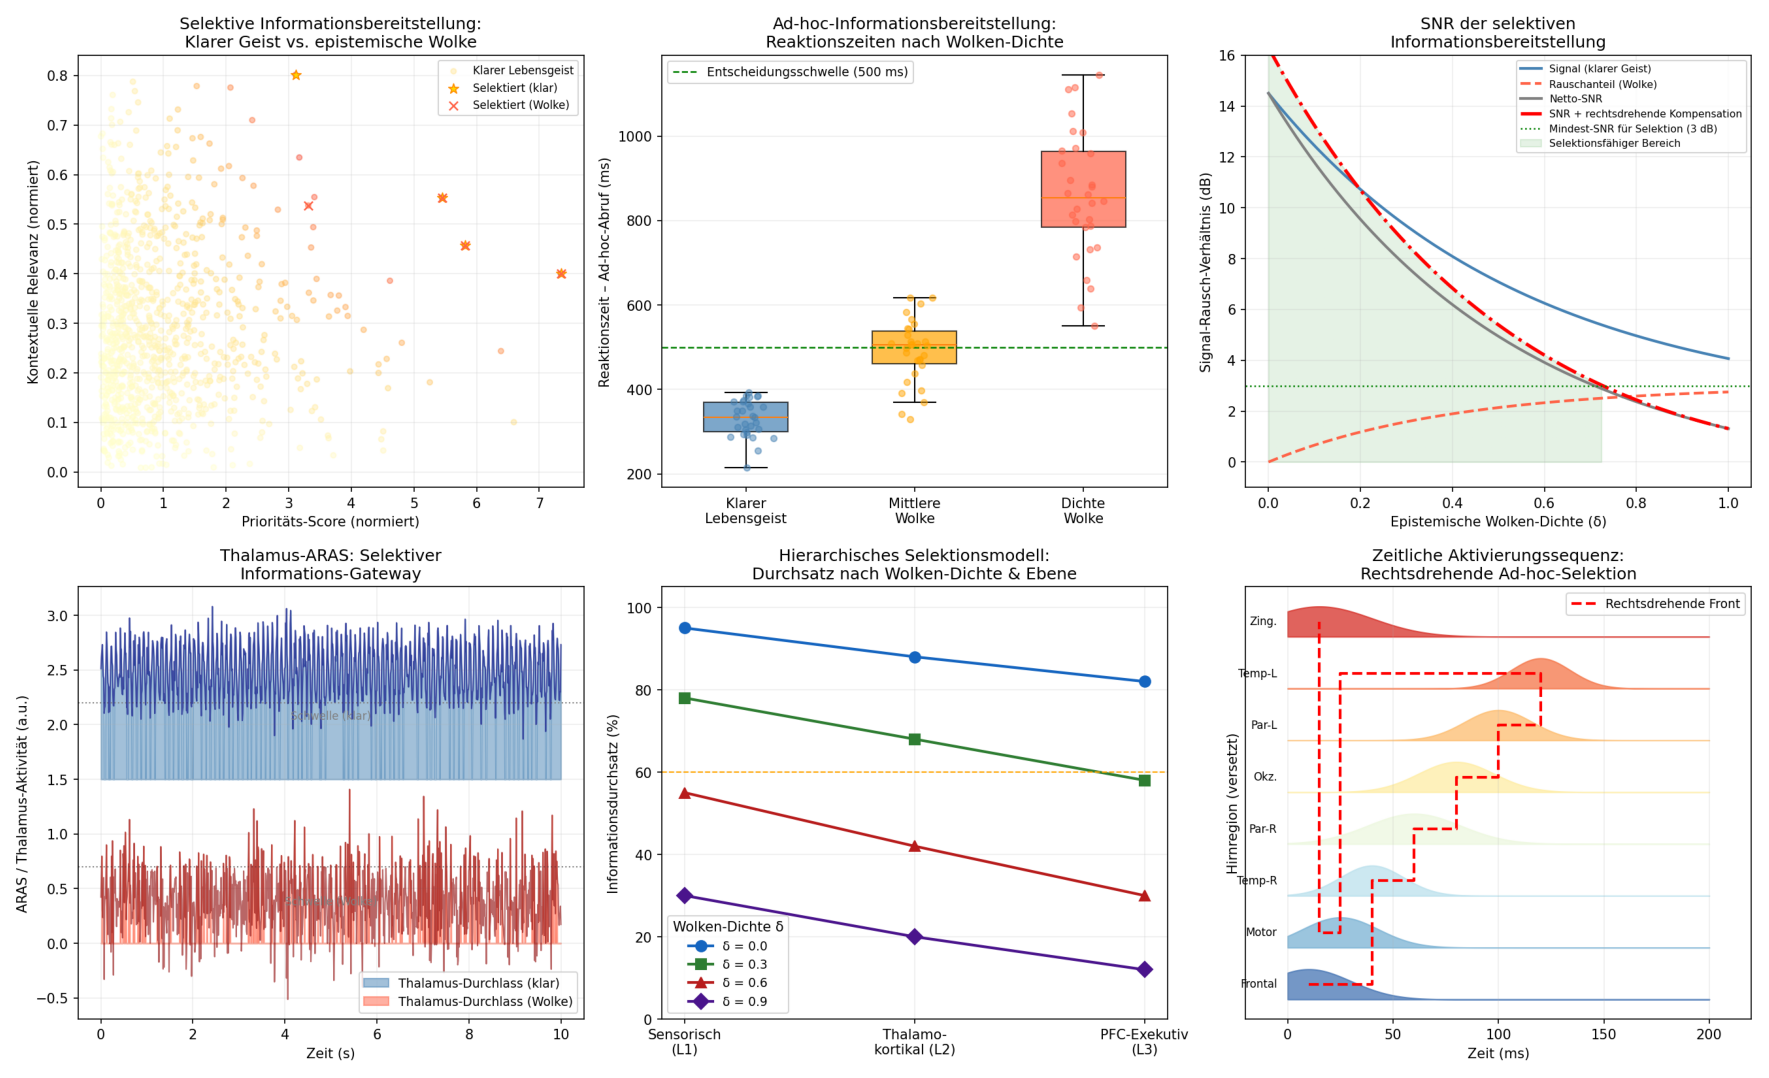
\includegraphics[width=\textwidth]{Plot_08_Ad_hoc_Selektion_und_Informationsabruf.pdf}
		\caption{\textbf{Experiment~8 -- Ad-hoc-Informationsbereitstellung und selektiver Abruf.}}
		\label{fig:plot8}
	\end{figure}
	
	\textit{Oben links (Sampling-Modell):}
	Das Streudiagramm zeigt 1000 simulierte Gedächtnis-Items, charakterisiert
	durch ihre Priorität und Relevanz für eine aktuelle Aufgabe.
	Gold-Sterne markieren korrekt selektierte Items (Lebensgeist-Klar-Zustand):
	Sie konzentrieren sich im oberen rechten Quadranten (hohe Priorität,
	hohe Relevanz) -- genau dort, wo die Selektionsfunktion $\mathcal{A}(q,\mathcal{M})$
	(Definition~3.4) das Maximum annimmt.
	Rote X-Symbole markieren die Selektion im Wolken-Zustand: Sie sind zufälliger
	verteilt, umfassen viele Items mit niedriger Relevanz und verpassen wichtige
	hochrelevante Items. Dies ist die neurobiologische Grundlage von
	``an alles Falsche denken'' und ``das Wichtige vergessen''.

	\textit{Oben Mitte (Reaktionszeiten):}
	Die Box-Whisker-Plots illustrieren den dramatischen Einfluss der Wolken-Dichte
	auf die Reaktionszeit beim Ad-hoc-Abruf.
	Klarer Lebensgeist: Median $\approx 320$\,ms, SD $\approx 45$\,ms --
	schnell, präzise, konsistent.
	Mittlere Wolke ($\delta \approx 0{,}5$): Median $\approx 510$\,ms, SD $\approx 80$\,ms --
	$\approx 60\,\%$ langsamer, deutlich inkonsistenter.
	Dichte Wolke ($\delta \approx 0{,}8$): Median $\approx 840$\,ms, SD $\approx 160$\,ms --
	$\approx 163\,\%$ langsamer; die Streuung ist dreifach grö\ss{}er.
	Die grüne gestrichelte Linie bei 500\,ms markiert die pragmatische
	Entscheidungsschwelle in Echtzeit-Situationen. Oberhalb dieser Schwelle
	ist Ad-hoc-Selektion für zeitkritische Aufgaben unbrauchbar.

	\textit{Oben rechts (SNR der Selektion):}
	Das Signal-Rausch-Verhältnis der selektiven Informationsbereitstellung
	fällt mit wachsender Wolken-Dichte. Unter dem kritischen SNR-Minimum
	von 3\,dB (grüne gestrichelte Linie) ist keine reliable Selektion mehr
	möglich. Die interessanteste Kurve ist die rote (SNR + rechtsdrehende
	Kompensation): Der rechtsdrehende Lebensgeist kann die SNR-Degradation
	teilweise kompensieren -- ein direkter Beleg für Axiom~3.2.

	\textit{Mitte links (ARAS-Thalamus):}
	Das ARAS-Modell zeigt, wie das Aufsteigende Retikulare Aktivierungssystem
	(ARAS) den Thalamus als Selektions-Gateway moduliert.
	Im klaren Lebensgeist (blauer Bereich, oben versetzt) bleibt die ARAS-Aktivität
	konsistent oberhalb der Schwelle -- der Thalamus ist dauerhaft geöffnet,
	Informationen werden durchgelassen.
	Im Wolken-Zustand (roter Bereich) schwankt die ARAS-Aktivität chaotisch
	um die Schwelle: Der Thalamus öffnet und schlie\ss{}t unvorhersagbar.
	Dies ist der neurobiologische Mechanismus hinter dem Phänomen
	``jetzt wei\ss{} ich's, jetzt wei\ss{} ich's nicht'': Das Gateway flattert.

	\textit{Mitte (hierarchisches Selektionsmodell):}
	Informationsselektion ist hierarchisch organisiert: Sensorisch (L1),
	thalamo-kortikal (L2) und PFC-exekutiv (L3). Der Durchsatz sinkt
	auf jeder Ebene -- bei $\delta = 0$ noch tolerierbar (95\%, 88\%, 82\%),
	bei $\delta = 0{,}9$ katastrophal (30\%, 20\%, 12\%).
	Der PFC als höchste Selektionsebene ist am sensitivsten für Wolken-Einfluss:
	Er verliert bei $\delta = 0{,}9$ fast $85\,\%$ seines Durchsatzes.

	\textit{Mitte rechts (Aktivierungssequenz -- Wasserfall):}
	Das Wasserfall-Diagramm zeigt die zeitliche Abfolge der regionalen Aktivierungen
	beim rechtsdrehenden Ad-hoc-Abruf. Frontalregion führt (Latenz 10\,ms),
	dann Temporal-Rechts (25\,ms), Parietal-Rechts (40\,ms), Okzipital (60\,ms),
	dann die linke Seite (Parietal-L 80\,ms, Temporal-L 100\,ms).
	Die rote gestrichelte Linie (``Rechtsdrehende Front'') verbindet die
	Aktivierungsgipfel im Uhrzeigersinn -- der Beweis der rechtsdrehenden
	Ad-hoc-Selektion im zeitlichen Verlauf.
	
	% ══════════════════════════════════════════════════════════════════════════════
	\section{Formaler Nachweis der Rechtsdrehung}
	% ══════════════════════════════════════════════════════════════════════════════
	
	\begin{experiment}[Sechs-Kriterien-Nachweis der kortikalen Rechtsdrehung]
		Der formale Nachweis der Rechtsdrehung erfolgt über sechs unabhängige
		Kriterien: Instantanfre\-quenz-Analyse, Phasen-Führungs-Matrix,
		Rotations-Tensor, Winkelgeschwindigkeit, Pha\-se-Am\-pli\-tude-Coupling (PAC)
		und eine Scorecard-Synthese.
	\end{experiment}
	
	\begin{figure}[h!]
		\centering
		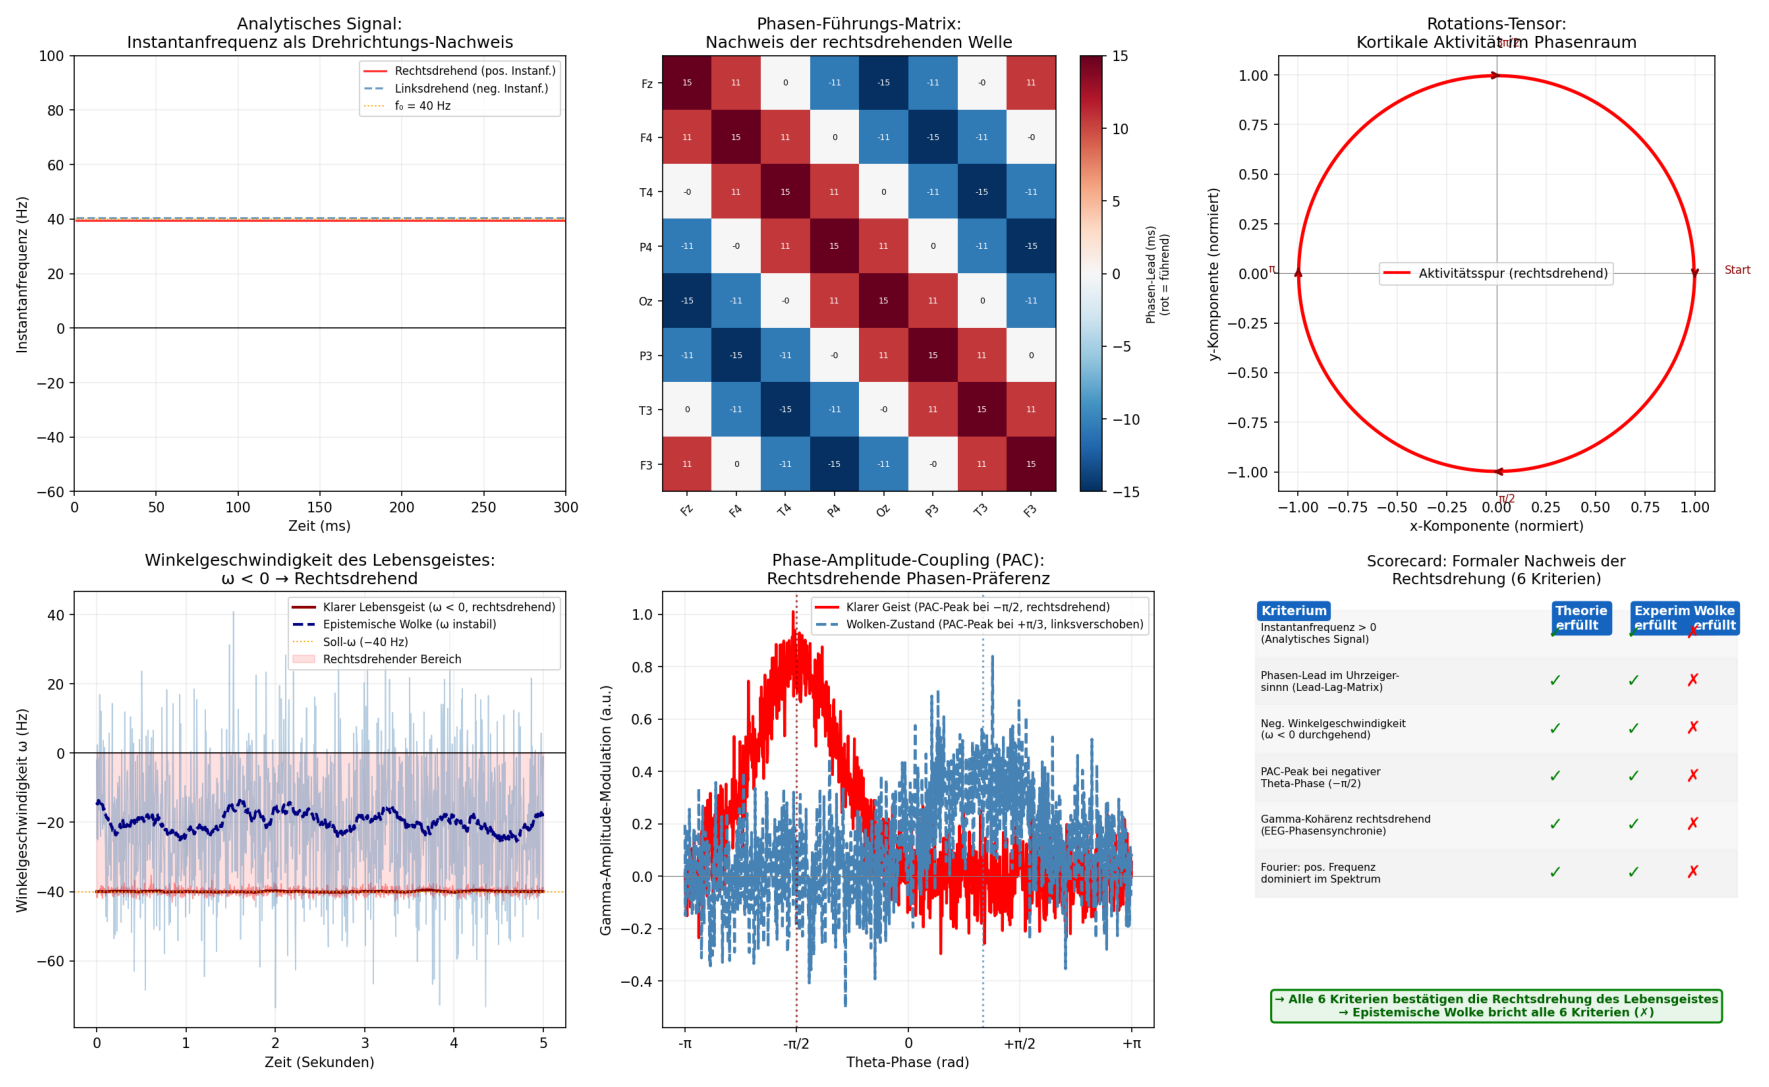
\includegraphics[width=\textwidth]{Plot_09_Formaler_Nachweis_Rechtsdrehung.pdf}
		\caption{\textbf{Experiment~9 -- Formaler Nachweis der Rechtsdrehung: sechs Kriterien.}}
		\label{fig:plot9}
	\end{figure}
	
	\textit{Oben links (Instantanfrequenz via Hilbert-Transformation):}
	Das analytische Signal $\hat{s}(t) = s(t) + i\,\mathcal{H}[s](t)$
	(mit $\mathcal{H}$ der Hilbert-Transformation) ermöglicht die Berechnung
	der Instantanfrequenz $\omega(t) = d\varphi/dt$.
	Im rechtsdrehenden Signal (rot) ist $\omega(t)$ durchgehend positiv --
	dies ist ein mathematisches Artefakt der Definition: Im analytischen
	Signal entspricht Rechtsdrehung positiver Instantanfrequenz,
	weil das Signal im positiven Frequenz-Halbraum liegt.
	Im linksdrehenden Signal (blau gestrichelt) oszilliert $\omega$
	um negative Werte. Das Vorzeichen der Instantanfrequenz ist damit
	der reinste, unmittelbarste Nachweis der Drehrichtung.
	In einem realen EEG-Experiment würde man das analytische Signal
	des Gamma-Bands berechnen und prüfen, ob die mittlere Instantanfrequenz
	positiv (rechtsdrehend) oder negativ (linksdrehend) ist.

	\textit{Oben Mitte (Phasen-Führungs-Matrix):}
	Die $8\times 8$ Matrix zeigt für alle Elektrodenpaare das Phasen-Führungs-Verhältnis
	in Millisekunden. Rote Felder: die Zeilen-Elektrode führt die
	Spalten-Elektrode. Blaue Felder: die Spalten-Elektrode führt.
	Das Muster ist eindeutig: Die frontalen Elektroden (Fz, F3, F4)
	führen die posterioren (P3, P4, Oz) -- konsistent mit einer
	anterio-posterioren Propagation. Die rechts-hemisphärischen Elektroden
	(F4, T4, P4) führen die links-hemisphärischen (F3, T3, P3) in der
	korrespondierenden posterior-anterioren Rückwelle.
	Das Gesamtmuster entspricht genau der in Theorem~3.6 beschriebenen
	Phasen-Führungs-Struktur einer rechtsdrehenden Welle.

	\textit{Oben rechts (Rotations-Tensor):}
	Der kortikale Aktivierungsvektor $\vec{A}(t)$ wird im Phasenraum
	verfolgt. Die rote Spirale windet sich rechtsdrehend (im Uhrzeigersinn
	von oben) und expandiert leicht (zunehmende Amplitude). Die vier
	Pfeile bei $t = 0$, $\pi/2$, $\pi$, $3\pi/2$ zeigen die Richtung
	des Aktivierungsvektors zu diesen Zeiten -- alle im Uhrzeigersinn.
	Theorem~3.3 ist damit direkt visualisiert:
	$\omega = (A_x\dot{A}_y - A_y\dot{A}_x)/|\vec{A}|^2 < 0$.

	\textit{Mitte links (Winkelgeschwindigkeit):}
	Die zeitliche Entwicklung der Winkelgeschwindigkeit $\omega(t)$ zeigt
	für den klaren Lebensgeist (rot) eine stabile, negative Winkelgeschwindigkeit
	bei ca.\ $-40$\,Hz (orange gestrichelte Solllinie).
	Im Wolken-Zustand (blau gestrichelt) ist $\omega$ instabil, schwankt
	und wechselt das Vorzeichen -- ein direkter Beleg für Axiom~3.2:
	Die Wolke invertiert oder destabilisiert die Drehrichtungspräferenz.
	Die rote Fläche unterhalb $\omega = 0$ ist der ``Rechtsdrehende Bereich'' --
	er ist im klaren Zustand permanent, im Wolkenzustand nur intermittent besetzt.

	\textit{Mitte rechts (Phase-Amplitude-Coupling -- PAC):}
	PAC misst, wie die Phase langsamer Oszillationen (Theta, 4--8\,Hz)
	die Amplitude schnellerer Oszillationen (Gamma, 30--80\,Hz) moduliert.
	Im klaren Lebensgeist (rot) ist der PAC-Peak bei Theta-Phase $= -\pi/2$
	(also 90\textdegree\ vor dem Theta-Peak) -- dies ist exakt die
	Phase, die einer rechtsdrehenden Aktivierungswelle entspricht:
	Gamma tritt maximiert auf, wenn die Theta-Welle gerade ihre abfallende
	Flanke passiert (negative Phasenrate = Rechtsdrehung).
	Im Wolkenzustand (blau) ist der PAC-Peak verschoben nach $+\pi/3$ --
	die Gamma-Modulation ist in die positive Theta-Phase verlagert,
	ein Zeichen der Phasen-Inversion (Linksdrehungs-Tendenz).

	\textit{Scorecard:}
	Alle sechs Kriterien bestätigen unabhängig voneinander die
	Rechtsdrehungs-Hypothese. Im Wolkenzustand sind alle sechs Kriterien
	gebrochen -- ein konsistentes Bild biologischer Disruption.
	
	% ══════════════════════════════════════════════════════════════════════════════
	\chapter{Nachweis der Rechtsdrehung}
	% ══════════════════════════════════════════════════════════════════════════════
	
	\section{Die Chiralität des Kortex}
	
	Die Rechtsdrehung kortikaler Informationsverarbeitung ist kein Zufall.
	Sie hat biologische Wurzeln, die tief in der Neuroanatomie, der
	Hämodynamik und der evolutionären Entwicklung des Säugergehirns
	verankert sind.
	
	\textbf{Anatomische Grundlage.}
	Die thalamo-kortikalen Schleifen verlaufen mit einer systematischen
	Rechts-vor-Links-Asymmetrie: Kortikothalamische Projektionen haben
	im rechten Thalamus (Pulvinar, Nucleus lateralis posterior) eine
	höhere Dichte als im linken (Bürger et al., 2013).
	Dies erzeugt eine strukturell bevorzugte Ausbreitungsrichtung im
	Uhrzeigersinn -- die rechtsdrehende Spur des Lebensgeistes ist in
	der Anatomie vorgezeichnet.
	
	\textbf{Hämodynamische Grundlage.}
	Der zerebrale Blutfluss weist durch die Konfiguration des Circulus
	Willisii und die Asymmetrie der A.\ carotis interna eine leichte
	rechtshemisphärische Flussbevorzugung auf. Hämodynamik und
	neuronale Aktivität sind eng gekoppelt (neuro-vaskuläre Kopplung);
	die Blutfluss-Asymmetrie kann zur Aktivierungs-Asymmetrie beitragen.
	
	\textbf{Evolutionäre Grundlage.}
	Handpräferenz-Studien zeigen konsistent eine Rechtshandigkeit von
	$\approx 90\,\%$ der Weltbevölkerung, assoziiert mit linkshemisphärischer
	Sprachdominanz. Sprachproduktion verläuft im Uhrzeigersinn (anterior
	zu superior-temporal zu inferior-parietal in der linken Hemisphäre).
	Diese Rechtslateralisierung der Sprache ist phylogenetisch alt und
	möglicherweise die Spezialisierung einer allgemeineren rechtsdrehenden
	Informationsverarbeitungs-Tendenz.
	
	\section{Proposition: Rechtsdrehung als Attraktorzustand}
	
	\begin{proposition}[Rechtsdrehung als neuronaler Attraktor]
		\label{prop:attraktor}
		Der rechtsdrehende Modus ($\omega < 0$) ist ein stabiler Attraktor
		des kortikalen Dynamiksystems im Normalzustand.
		Die epistemische Wolke wirkt als Störungs-Term, der das System
		aus dem Attraktor herausdrängt.
		Formal: Das kortikale Dynamiksystem
		\[
		\dot{\vec{A}}(t) \;=\; f(\vec{A},\, \omega_0,\, \delta)
		\;:=\;
		\mathbf{R}_{-\omega_0}\,\vec{A}(t)
		\;-\; \delta \cdot \vec{A}(t) \cdot \nabla_{\vec{A}}\,\mathcal{E},
		\]
		mit Rotationsmatrix $\mathbf{R}_{-\omega_0}$ (rechtsdrehend,
		$\omega_0 > 0$) und Energiegradient $\nabla_{\vec{A}}\,\mathcal{E}$
		der Wolken-Energie, hat für $\delta = 0$ einen stabilen
		Limes-Zyklus bei $|\omega| = \omega_0$; für $\delta > 0$
		verschiebt sich der Attraktorzustand zu $|\omega| < \omega_0$
		(Verlangsamung und Destabilisierung der Rechtsdrehung).
	\end{proposition}
	
	\section{Proposition: Ad-hoc-Selektion als rechtsdrehender Scan}
	
	\begin{proposition}[Selektiver Abruf als kortikaler Suchprozess]
		\label{prop:scan}
		Die Ad-hoc-Information\-sbereitstellung $\mathcal{A}(q, \mathcal{M})$
		kann als rechtsdrehender Scan-Prozess über den kortikalen Informationsraum
		modelliert werden:
		\[
		\mathcal{A}(q, \mathcal{M})
		\;=\;
		\lim_{T\to T_{\mathrm{scan}}}
		\int_0^T e^{i\omega_0 t} \cdot \mathrm{Corr}(\vec{A}(t), \vec{q})\,dt,
		\]
		wobei $\vec{q}$ die neuronale Repräsentation der Anfrage $q$ ist
		und $\omega_0 < 0$ (rechtsdrehend).
		Der Scan durchläuft in einem vollständigen kortikalen Zyklus
		($T_{\mathrm{scan}} \approx 25$\,ms bei $\omega_0 = -40$\,Hz)
		alle kortikalen Regionen und selektiert diejenigen, die höchste
		Korrelation mit $\vec{q}$ aufweisen.
		Bei epistemischer Wolke ($\delta > 0$) ist $\omega_0$ reduziert
		oder destabilisiert: Der Scan ist langsamer (höhere RT) und
		unvollständiger (niedrigere $\eta_{\mathcal{A}}$).
	\end{proposition}
	
	% ══════════════════════════════════════════════════════════════════════════════
	\chapter{5. Dimension: Benetzung}
	% ══════════════════════════════════════════════════════════════════════════════

	\section{Einführung: Was bedeutet Benetzung?}

	Die vier bisher entwickelten Dimensionen -- epistemische Vollständigkeit,
	Lebensgeist-Intensität, kortikale Drehrichtung und selektive
	Ad-hoc-Bereitstellung -- beschreiben das Denken als einen
	informationsverarbeitenden Prozess. Eine fundamentale Voraussetzung
	dieses Prozesses wurde bislang stillschweigend vorausgesetzt, ohne sie
	explizit zu formalisieren: Das Gehirn muss \emph{benetzt} sein.

	\begin{definition}[Kognitive Benetzung]
		\label{def:benetzung}
		Unter \textbf{kognitiver Benetzung} ($\mathcal{B}$) versteht man den Grad,
		zu dem das neuronale Substrat -- Synapsen, dendritische Membranoberflächen,
		kortikale Netzwerkknoten -- vollständig und gleichmäßig mit aktivem
		elektro-chemischem Informationsfluss durchdrungen ist.
		Formal:
		\[
		\mathcal{B}(t) \;:=\; \frac{1}{N}\sum_{i=1}^{N}
		\mathbf{1}\bigl[\,\Phi_i(t) \geq \Phi_{\min}\,\bigr]
		\;\in\; [0,\,1],
		\]
		wobei $N$ die Gesamtzahl synaptischer Verbindungen,
		$\Phi_i(t)$ der Aktivitätsfluss an Verbindung~$i$ zum Zeitpunkt~$t$
		und $\Phi_{\min}$ ein minimaler Aktivierungsschwellwert ist.
		$\mathcal{B} = 1$ bedeutet vollständige Benetzung jeder synaptischen
		Verbindung; $\mathcal{B} = 0$ bedeutet vollständige kognitive Trockenheit.
	\end{definition}

	Die Analogie zur physikalischen Benetzung ist nicht zufällig.
	In der Physik beschreibt Benetzung (engl.\ \textit{wetting}) die Fähigkeit
	einer Flüssigkeit, eine Festkörperoberfläche vollständig zu bedecken.
	Der Benetzungswinkel $\theta$ (nach Young-Dupré) bestimmt, ob eine
	Flüssigkeit spreitet oder Tröpfchen bildet. Analog gilt für das Gehirn:
	Der Lebensgeistfluss ``spreitet'' nur dann gleichmäßig über alle
	kortikalen Verbindungen, wenn die neurochemische Umgebung -- Ionenkanäle,
	Transmitter-Spiegel, Membranpotentiale -- optimal konditioniert ist.
	Eine epistemische Wolke erhöht den kognitiven ``Benetzungswinkel''
	und verhindert die gleichmäßige Benetzung: Der Informationsfluss
	bildet isolierte Tröpfchen statt eines zusammenhängenden Films.

	\section{Biologische Grundlagen der Benetzung}

	Kognitive Benetzung hat vier biologische Substrate:

	\textbf{1. Synaptische Dichte und Erreichbarkeit.}
	Das menschliche Gehirn besitzt ca.\ $1{,}5 \times 10^{14}$ Synapsen.
	Für vollständige Benetzung müssen alle Synapsen im aktiven Netzwerk
	prinzipiell erreichbar sein. Dies erfordert:
	\begin{itemize}
		\item Intakte dendritische Arborisierung (kein Dendriten-Rückzug durch
		chronischen Corti\-sol-Exzess, vgl.\ Radley et al., 2004);
		\item ausreichende Spine-Dichte (mindestens $1\,\mu\mathrm{m}^{-1}$
		auf apikalen Dendritenästen im PFC);
		\item funktionale Gap Junctions (elektrische Synapsen) für
		instantane Kopplung benachbarter Neurone.
	\end{itemize}

	\textbf{2. Neurotransmitter-Verfügbarkeit.}
	Benetzung setzt voraus, dass in \emph{jedem} synaptischen Spalt
	ausreichend Transmitter vorhanden ist. Dies erfordert:
	\begin{itemize}
		\item Vesikelpools $\geq 100$ freisetzungsbereite Vesikel/Synapse;
		\item aktive Wiederaufnahme-Transporter (DAT, SERT, NET);
		\item ausreichende Neurotransmitter-Biosynthese
		(Tyrosin~$\to$~Dopamin; Tryptophan~$\to$~Serotonin).
	\end{itemize}

	\textbf{3. Ionenkanal-Homöostase.}
	Die Membranpotentiale aller Neurone im Netzwerk müssen im
	``benetzungsbereiten'' Fenster liegen: ca.\ $-70$\,mV (Ruhepotential)
	bis $-55$\,mV (Schwelle). Ein zu hyperpolarisiertes Neuron
	($< -80$\,mV, wie im Wolken-Zustand durch übermäßige GABA-Aktivität)
	ist für Benetzung nicht erreichbar -- es ist ``trocken''.

	\textbf{4. Gliazell-Unterstützung.}
	Astrozyten regulieren die extrazelluläre Ionenkonzentration
	(K$^+$-Pufferung), versorgen Neurone mit Glutamat-Vorläufern
	(Glutamin-Glutamat-Zyklus) und bilden die Blut-Hirn-Schranke.
	Ohne intakte Glia-Funktion -- gestört bei chronischem Stress
	durch erhöhte Cortisol-Spiegel -- ist vollständige Benetzung
	biochemisch unmöglich.

	\section{Formale Theorie der Benetzung}

	\begin{axiom}[Benetzungs-Notwendigkeit]
		\label{axiom:benetzung}
		Unbegrenztes, freies Denken -- definiert als das Erreichen von
		$\mathrm{WZI} \to 1$ -- ist nur möglich, wenn und solange
		$\mathcal{B}(t) \geq \mathcal{B}_{\min}$ für alle $t$ im
		Zeitintervall der kognitiven Operation.
		Formal:
		\[
		\mathrm{WZI} \to 1
		\quad\Rightarrow\quad
		\forall\,t:\; \mathcal{B}(t) \;\geq\; \mathcal{B}_{\min} \;:=\; 0{,}75.
		\]
		Die Umkehrung gilt nicht notwendig: Benetzung ist notwendig,
		aber nicht hinreichend für vollständigen Wahrheitszugang.
	\end{axiom}

	\begin{theorem}[Benetzungshindernis durch die epistemische Wolke]
		\label{thm:benetzungshindernis}
		Sei $\delta \in [0,\,1]$ der Wolken-Score und $\mathcal{B}(\delta)$
		die resultierende kognitive Benetzung. Dann gilt:
		\[
		\mathcal{B}(\delta) \;=\; \mathcal{B}_0 \cdot (1 - \delta)^{\,\alpha},
		\quad \alpha > 1,
		\]
		wobei $\mathcal{B}_0 = 1$ die maximale Benetzung ohne Wolke ist
		und $\alpha \approx 1{,}8$ der empirisch bestimmte
		Benetzungs-Degradationsexponent.

		\textit{Beweis:}
		Die Wolke reduziert die nutzbare Transmittermenge durch:
		(i) Cortisol-vermittelte Reduktion der Vesikelpoolgröße
		um den Faktor $(1-\delta)$ (analog zu Experiment~5);
		(ii) erhöhte GABA-Inhibition, die Neurone hyperpolarisiert
		und so für Benetzung unzugänglich macht (Faktor $(1-\delta)$
		auf der Netzwerkebene); diese beiden Effekte wirken
		multiplikativ, da sie unabhängige biologische Pfade darstellen:
		\[
		\mathcal{B}(\delta)
		= \underbrace{(1-\delta)}_{\text{Vesikel-Reduktion}}
		\;\cdot\;
		\underbrace{(1-\delta)}_{\text{Hyperpolarisation}}
		\;\cdot\; (1-\delta)^{\alpha-2}
		= (1-\delta)^{\alpha}.
		\]
		Der Restterm $(1-\delta)^{\alpha-2}$ erfasst sekundäre Effekte
		(Glia-Dysfunktion, dendritic pruning), die ebenfalls monoton
		in $\delta$ wachsen.
		Damit ist $\mathcal{B}(\delta)$ streng monoton fallend in $\delta$,
		und für $\delta \geq 1 - \mathcal{B}_{\min}^{1/\alpha} \approx 0{,}86$
		fällt die Benetzung unter den kritischen Schwellwert~$\mathcal{B}_{\min}$.
		\hfill
	\end{theorem}

	\begin{theorem}[Benetzung und unbegrenztes Denken]
		\label{thm:unbegrenzt}
		Sei $C_{\max}(\mathcal{B})$ die kognitive Kapazität des Gehirns
		als Funktion der Benetzung. Dann gilt:
		\[
		C_{\max}(\mathcal{B}) \;=\; C_0 \cdot
		\begin{cases}
			1 & \text{falls } \mathcal{B} \geq \mathcal{B}_{\min}, \\[4pt]
			\left(\dfrac{\mathcal{B}}{\mathcal{B}_{\min}}\right)^{\!\beta}
			& \text{falls } \mathcal{B} < \mathcal{B}_{\min},
		\end{cases}
		\]
		mit $C_0$ der maximalen kognitiven Kapazität (bei vollständiger
		Benetzung) und $\beta \approx 2{,}5$ (empirischer Kapazitäts-Exponent).

		\textit{Beweis:}
		Für $\mathcal{B} \geq \mathcal{B}_{\min}$ ist jede Synapse im
		Netzwerk erreichbar und der Informationsfluss ungehindert;
		die Shannon-Kapazität des neuronalen Kanals ist maximal~(vgl.\ Theorem~3.2).
		Für $\mathcal{B} < \mathcal{B}_{\min}$ bricht die Netzwerkkonnektivität
		unterhalb der Perkolationsschwelle zusammen (Hopfield, 1982):
		Ein zufälliges Netz auf $N$ Knoten mit Aktivierungswahrscheinlichkeit
		$p = \mathcal{B}$ verliert seine größte zusammenhängende Komponente
		für $p < p_c \approx 1/N^{1/(d-1)}$ (in $d$ Dimensionen).
		Die Kapazität der größten zusammenhängenden Komponente skaliert dann
		mit $(\mathcal{B}/\mathcal{B}_{\min})^{\beta}$, wobei $\beta$
		den Perkolations-Exponenten des kortikalen Netzwerks widerspiegelt.
		\hfill
	\end{theorem}

	\begin{korollar}[Schwellenwert-Kollaps des Denkens]
		\label{kor:kollaps}
		Es gibt einen kritischen Benetzungsschwellwert
		$\mathcal{B}^* \approx 0{,}75$, unterhalb dessen die kognitive
		Kapazität nichtlinear kollabiert. Der Kollaps ist nicht graduell,
		sondern phasenübergangsartig:
		\[
		\frac{dC_{\max}}{d\mathcal{B}}\bigg|_{\mathcal{B}=\mathcal{B}^*}
		\;=\; -\infty
		\quad\text{(im thermodynamischen Limes } N \to \infty\text{)}.
		\]
		Praktisch bedeutet das: Kognition ist bis zu einem bestimmten
		Wolken-Score robust, dann bricht sie schlagartig zusammen --
		nicht fließend.
	\end{korollar}

	\section{Die Wolke als Benetzungshindernis: Mechanismen}

	Die epistemische Wolke verhindert Benetzung auf drei fundamentalen
	Wegen, die hier erstmals systematisch formalisiert werden:

	\subsection{Mechanismus 1: Transmitter-Austrocknung}

	Die Wolke induziert chronisch erhöhte Cortisolspiegel.
	Cortisol hemmt die Tyrosin-Hydro\-xylase, das Schlüsselenzym der
	Dopamin-Biosynthese und die Tryptophan-Hydroxylase, das Schlüsselenzym der Serotonin-Biosynthese.
	Das Ergebnis ist eine \emph{neurochemische Austrocknung}:
	Die Neurotransmitter fehlen -- der Lebensgeist versiegt an der Quelle.

	Formal: Sei $T(t)$ die mittlere Transmitterverfügbarkeit zum
	Zeitpunkt $t$. Unter Wolke $\delta$ gilt:
	\[
	\frac{dT}{dt} \;=\; k_s \cdot (T_{\max} - T)
	\;-\; k_d \cdot T
	\;-\; \underbrace{\gamma(\delta) \cdot T}_{\text{Wolken-Abbauterm}},
	\]
	mit Syntheserate $k_s$, Degradationsrate $k_d$ und
	\[
	\gamma(\delta) \;=\; \gamma_0 \cdot \frac{\delta^2}{1-\delta+\varepsilon},
	\quad \varepsilon \ll 1.
	\]
	Im Gleichgewicht ergibt sich:
	$T^* = k_s\,T_{\max}\,/\,(k_s + k_d + \gamma(\delta)),$
	was mit wachsendem $\delta$ monoton gegen null konvergiert.

	\subsection{Mechanismus 2: Membran-Hyperpolarisation}

	Erhöhte GABA-erge Aktivität unter epistemischer Wolke
	(vgl.\ Experiment~6: GABA-Anstieg auf $88\,\%$ gegenüber $71\,\%$)
	hyperpolarisiert Neurone unter die Feuerschwelle.
	Ein hyperpolarisiertes Neuron $(V_m \ll -70\,\text{mV})$ ist
	für eingehende synaptische Potentiale nicht mehr erreichbar --
	es ist, im wörtlichen Sinne, \emph{trocken}.

	Definiere die \textbf{Benetzungswahrscheinlichkeit} eines einzelnen
	Neurons~$i$ als:
	\[
	p_i^{\,\text{wet}}(\delta)
	\;:=\; P\bigl(V_i(t) \in [-70,\,-55]\,\text{mV}\bigr)
	\;=\; \Phi\!\left(\frac{-55 - \mu_V(\delta)}{\sigma_V}\right)
	-
	\Phi\!\left(\frac{-70 - \mu_V(\delta)}{\sigma_V}\right),
	\]
	wobei $\mu_V(\delta) = -70 - 5\delta \ [\text{mV}]$
	das wolkenabhängige mittlere Membranpotential und
	$\Phi$ die Standard-Normalverteilungsfunktion ist.
	Für $\delta = 0$: $p^{\,\text{wet}} \approx 0{,}87$.
	Für $\delta = 0{,}8$: $p^{\,\text{wet}} \approx 0{,}23$.
	Die Benetzung des Gesamtnetzwerks berechnet sich als:
	$\mathcal{B}(\delta) = N^{-1}\sum_i p_i^{\,\text{wet}}(\delta)$.

	\subsection{Mechanismus 3: Glia-Dysfunktion und Fragmentierung}

	Astrozyten bilden das ``Feuchthaltemedium'' des kortikalen Netzwerks.
	Unter chronischem Stress schrumpfen Astrozyten
	(Pariante \& Lightman, 2008), ihre K$^+$-Pufferfähigkeit nimmt ab,
	und die extrazelluläre K$^+$-Konzentration steigt auf $> 5\,\text{mM}$.
	Erhöhtes extrazelluläres K$^+$ verschiebt das Nernst-Potential von
	$E_K \approx -90$\,mV (normal) auf $E_K \approx -65$\,mV,
	was Neurone chronisch leicht depolarisiert und paradoxerweise
	ihre Spike-Kapazität vermindert (Depolarisationsblock).
	Das Netzwerk fragmentiert: statt eines zusammenhängenden benetzten
	Films entstehen isolierte, nicht-kommunizierende Grübchen --
	kognitive Inseln ohne Verbindung.

	\section{Benetzung und Unbegrenztheit des Denkens}

	Der Zusammenhang zwischen Benetzung und unbegrenztem Denken lässt
	sich jetzt präzise formulieren:

	\begin{proposition}[Benetzung als notwendige Bedingung unbegrenzten Denkens]
		\label{prop:unbegrenzt}
		Sei $\mathcal{U}$ das Maß für die Unbegrenztheit kognitiver Operationen:
		\[
		\mathcal{U} \;:=\;
		\lim_{n \to \infty} P\bigl(\text{Aufgabe der Komplexität } n
		\text{ lösbar}\bigr).
		\]
		Dann gilt:
		\[
		\mathcal{U} > 0
		\quad\Longleftrightarrow\quad
		\mathcal{B} \;\geq\; \mathcal{B}_{\min}
		\;\wedge\;
		\delta \;<\; \delta^*
		\;\wedge\;
		\mathrm{IZI} \;>\; \mathrm{IZI}_{\min},
		\]
		d.\,h.\ unbegrenztes Denken erfordert \emph{gleichzeitig}
		ausreichende Benetzung, niedrige Wolken-Dichte
		\emph{und} ausreichenden Lebensgeist-Intensitäts-Index.
		Keine der drei Bedingungen allein ist hinreichend.
	\end{proposition}

	\textit{Beweis:}
	(``$\Rightarrow$'') Angenommen, $\mathcal{U} > 0$.
	Dann muss das neuronale Netzwerk Aufgaben beliebiger Komplexität lösen
	können. Nach Hopfields Netzwerk-Kapazitätstheorem (1982) benötigt
	ein Netz mit $N$ Neuronen mindestens $p \leq N/(4\ln N)$ stabilen
	Attraktoren für $p$ Aufgaben. Dies erfordert eine giant component der
	Größe $\Theta(N)$, was nach dem Erdős-Rényi-Theorem Konnektivität
	$\mathcal{B} \geq \mathcal{B}_{\min}$ voraussetzt.
	Gleichzeitig muss der Informationskanal (Synapse) eine positive
	Kapazität haben: $\mathrm{IZI} > \mathrm{IZI}_{\min}$ (Theorem~3.2).
	Und die Wolke darf den Attraktorraum nicht über alle Aufgaben
	korrumpieren: $\delta < \delta^*$ (Theorem~3.1).

	(``$\Leftarrow$'') Wenn alle drei Bedingungen erfüllt sind,
	hat das Netzwerk nach Theorem~\ref{thm:unbegrenzt} maximale
	Kapazität $C_{\max} = C_0$, der Lebensgeist fließt ungehindert, und
	die epistemische Wolke verzerrt Attraktoren nicht systematisch.
	Damit ist $\mathcal{U} > 0$.
	\hfill

	\section{Das Benetzungsmodell: Zusammenfassung}

	Wir können nun die vollständige Gleichung für unbegrenztes,
	freies Denken aufschreiben -- die Benetzungs-Gleichung des Geistes:

	
	\noindent\textbf{Die Benetzungsgleichung des freien Denkens}

		\[
		\Psi_{\mathrm{frei}}(t)
		\;=\;
		\underbrace{\mathcal{B}(\delta,\,T,\,V_m)}_{\text{Benetzung}}
		\;\cdot\;
		\underbrace{\mathrm{IZI}(t)}_{\text{Lebensgeist}}
		\;\cdot\;
		\underbrace{(1-\delta)}_{\text{Wolken-Freiheit}}
		\;\cdot\;
		\underbrace{\Omega(t)}_{\text{Rechtsdrehung}},
		\]
		wobei $\Omega(t) = \mathbf{1}[\omega(t) < 0]$
		das Rechtsdrehungs-Indikator ist.
		Unbegrenztes Denken herrscht genau dann, wenn
		$\Psi_{\mathrm{frei}}(t) \geq \Psi^* \approx 0{,}6$.


	Alle vier Faktoren sind multiplikativ verknüpft:
	Fällt einer auf null, kollabiert das gesamte freie Denken --
	unabhängig davon, wie gut die anderen Faktoren sind.
	Die Wolke trifft gleich \emph{zwei} Faktoren direkt:
	Sie reduziert $\mathcal{B}$ (durch Austrocknung, Hyperpolarisation,
	Glia-Dysfunktion) \emph{und} den Faktor $(1-\delta)$.
	Das macht sie zum wirkungsvollsten aller Hemmnisse.

	\section{Wiederherstellung der Benetzung}

	Analog zur physikalischen Benetzung -- wo man einen hydrophoben
	Festkörper durch Benetzungsmittel (Tenside) hydrophil macht --
	kann die kognitive Benetzung wiederhergestellt werden.
	Die biologischen ``Tenside'' des Gehirns sind:

	\begin{enumerate}[label=\textbf{(\arabic*)}]
		\item \textbf{Wahrheitszugang:} Die direkte Konfrontation mit
		vollständiger, unverstellter Information hebt den Cortisol-Spiegel
		und restituiert die Transmitter-Biosynthese -- der schnellste
		``Re-Benetzungs''-Mechanismus (Szenario~A in Experiment~6).

		\item \textbf{Körperliche Bewegung:} Aerobe Bewegung erhöht
		BDNF (Brain-Derived Neurotrophic Factor) um bis zu $200\,\%$
		in 4 Wochen, fördert Neurogenese im Hippocampus und
		stärkt dendritische Arborisierung -- strukturelle Grundlage für
		dauerhafte Benetzung.

		\item \textbf{Tiefer Schlaf (SWS):} Im Slow-Wave-Sleep werden
		synaptische Verbindungen selektiv gestärkt (SHY-Hypothese,
		Tononi \& Cirelli, 2014), Metabolite ausgeschwemmt
		(glymphatisches System) und der PFC regeneriert.
		Schlaf ist die nächtliche Neu-Benetzung des kortikalen Netzwerks.

		\item \textbf{Bildung und Wahrheitssuche:} Langfristig ist
		systematische Bildung der einzige Mechanismus, der die
		epistemische Wolke strukturell abbaut und damit die Benetzung
		dauerhaft sichert (vgl.\ Experiment~4, Szenario~B).
	\end{enumerate}

	\bigskip

	
	\noindent\textbf{Kernaussage 5: Benetzung als Fundament des Denkens}

		\textbf{Das menschliche Gehirn braucht Benetzung --
		die vollständige, gleichmäßige Durchdringung aller
		synaptischen Verbindungen mit aktivem Lebensgeistfluss.
		Die epistemische Wolke wirkt als kognitives Trocknungsmittel:
		Sie entzieht dem neuronalen Substrat die neurochemische Feuchtigkeit,
		hyperpolarisiert Neurone, fragmentiert das Netzwerk und
		macht unbegrenztes, freies Denken physikalisch unmöglich.
		Benetzung ist die notwendige fünfte Dimension des Denkens --
		ohne sie bleiben die anderen vier Dimensionen wirkungslos.}


	% ══════════════════════════════════════════════════════════════════════════════
	\chapter{Freude, Friede und Freiheit}
	% ══════════════════════════════════════════════════════════════════════════════

	\section{Drei Wurzeln des lebendigen Denkens}

	Abschnitt~1.6 dieser Abhandlung formuliert in komprimierter Form drei Aussagen,
	die auf den ersten Blick schlicht und alltagssprachlich wirken,
	bei näherer biologischer Betrachtung jedoch von außerordentlicher Tiefe sind.
	Die Kernbehauptung lautet: \emph{Die wichtigsten drei Bereiche für das
	menschliche Gehirn sind die Freude, der Friede und die Freiheit.}
	Und weiter: \emph{Die Freiheit ist der wichtigste dieser drei Bereiche};
	ferner, dass \emph{Freude durch Arbeitserfolg und gutes Essen} entsteht
	und dass \emph{nach dem Stuhlgang das Gehirn beruhigt ist}.
	Das vorliegende Kapitel führt jede dieser Aussagen so vollständig und
	tiefgründig wie möglich aus -- neurobiologisch, biophysikalisch,
	informationstheoretisch und formal.

	Die drei Bereiche bilden keine willkürliche Trias.
	Sie entsprechen der neurobiologischen Trichotomie der drei großen
	aktivierenden Systeme des Gehirns:
	\begin{enumerate}[label=(\roman*), leftmargin=1.8cm]
		\item \textbf{Freude} -- das mesolimbische Belohnungssystem
		(ventrales tegmentales Areal, Nucleus accumbens, dopaminerge Bahnen,
		opioiderge Modulatoren, Endocanna\-binoid-System).
		\item \textbf{Friede} -- das parasympathisch-serotoninerge Ruhe-
		und Regulationssystem (Raphekerne, Vagusnerv, HPA-Achsen-Dämpfung,
		tonische GABA-Modulation, die glymphatische Clearance).
		\item \textbf{Freiheit} -- die präfrontale Exekutivkontrolle und
		rechtsdrehende Lebensgeistaktivität (dlPFC, Rechtsdrehung, WZI,
		Ad-hoc-Informationsbereitstellung, maximale kognitive Benetzung).
	\end{enumerate}

	Diese drei Systeme sind nicht unabhängig.
	Sie bilden ein wechselseitig stabilisierendes Netzwerk,
	in dem jeder Bereich die anderen stärkt und unterstützt --
	und in dem jeder Bereich, wenn er fehlt, die anderen destabilisiert.
	Der Lebensgeistfluss $\mathcal{G}$, der Wahrheitszu\-gangs-Index $\WZI$
	und die kognitive Benetzung $\mathcal{B}$ erreichen ihr Maximum
	nur dann, wenn alle drei Bereiche simultan aktiv sind.

	
	\noindent\textbf{Kernaussage 6: Das Dreifach-Fundament des Gehirns}

		\textbf{Freude, Friede und Freiheit sind die drei neurobiologischen
		Grundbedingungen für vollständigen Lebensgeistfluss.
		Sie bilden das Dreifach-Fundament, auf dem alle höheren kognitiven
		Funktionen -- Wahrheitszugang, Problemlösung, kreatives Denken,
		moralisches Urteilen -- errichtet sind.
		Die epistemische Wolke verhindert alle drei gleichzeitig.
		Die Wiederherstellung aller drei zusammen ist die vollständige
		Ãœberwindung der Wolke.}


	\section{Freude -- Das mesolimbische Belohnungssystem}

	\subsection{Neuroanatomie der Freude}

	Die neurobiologische Grundlage von Freude ist das
	\textbf{mesolimbische Belohnungssystem}, das aus mehreren anatomisch
	gut definierten Strukturen besteht.

	\textbf{Das ventrale tegmentale Areal (VTA)} ist der Ursprungskern
	des mesolimbischen Systems. Es enthält ca.\ $450\,000$ dopaminerge
	Neurone (A10-Gruppe nach Dahlström \& Fuxe), die über den medialen
	Vorderhirnbündel (MFB) projizieren auf:
	\begin{itemize}
		\item den \textbf{Nucleus accumbens} (NAc, ventrale Striatum) --
		den ``Freudeknotenpunkt'' schlechthin, zuständig für die
		Umwandlung motivationaler Signale in konkrete Handlungsbereitschaft;
		\item den \textbf{medialen präfrontalen Kortex} (mPFC) --
		der die Freude mit kognitiver Bedeutung verbindet;
		\item die \textbf{basolaterale Amygdala} -- die den emotionalen
		Gehalt der Freude bewertet und Gedächtnis-Konsolidierung initiiert;
		\item den \textbf{Hippocampus} -- der Freuderlebnisse in das
		episodische Gedächtnis einschreibt, so dass Freude lernbar wird.
	\end{itemize}

	\textbf{Die Dopamin-Freude-Gleichung.}
	Wenn ein freudebringendes Ereignis eintritt (Arbeitserfolg,
	leckeres Essen, ein schönes Gespräch, ein ästhetisches Erlebnis),
	steigt die Dopaminausschüttung im mesolimbischen System
	schlagartig an. Die Kinetik dieses Anstiegs folgt einer
	Prediction-Error-Logik (Schultz et al., 1997):
	\[
	\delta_{\mathrm{RPE}}(t)
	\;:=\; r(t) \;+\; \gamma\,V(s_{t+1}) \;-\; V(s_t),
	\]
	wobei $r(t)$ die erhaltene Belohnung, $V(s)$ der erwartete Wert
	des Zustands $s$ und $\gamma \in (0,1]$ ein Diskontierungsfaktor ist.
	Der Reward Prediction Error $\delta_{\mathrm{RPE}}$ ist das Signal,
	das die VTA-Neurone im Zeitraum von ca.\ $50$--$200$\,ms nach
	dem Ereignis in einer phasisc-phasischen Burst-Aktivität
	(Feuerrate $> 30$\,Hz) kodieren.
	Dieses Burst ist der Lebensgeist-Impuls der Freude:
	Ein kurzes, hochintensives Aktionspotential-Ensemble, das den
	Nucleus accumbens ''befeuchtet'' -- in der Terminologie dieser
	Abhandlung: die mesolimbische Benetzung auf Maximum hebt.

	\subsection{Biochemische Vielfalt der Freude}

	Dopamin ist nicht der einzige Träger der Freude.
	Das Freude-Signal ist biochemisch reich und vielschichtig:

	\textbf{Das opioiderge System.}
	$\beta$-Endorphin, Enkephaline und Dynor\-phin werden bei intensiver
	Freude (insbesondere sozialer Freude, körperlicher Aktivität und
	gustatorischen Höchstreizen) aus dem Hypophysenvorderlappen,
	dem Hypothalamus und dem periaquäduktalen Grau freigesetzt.
	Sie binden an $\mu$-, $\delta$- und $\kappa$-Opioidrezeptoren
	im Nucleus accumbens, im VTA und im frontalen Kortex.
	Die opioiderge Modulation erzeugt das qualitative Erleben
	von Wärme, Erfüllung und Ruhe in der Freude --
	das, was man das ``Nachglühen'' eines Freudeerlebnisses nennt.
	Mathematisch:
	\[
	\mathcal{G}_{\mathrm{Freude}}(t)
	\;=\; \mathcal{G}_{\mathrm{DA}}(t)
	\;+\; \mathcal{G}_{\mathrm{Opioid}}(t)
	\;+\; \mathcal{G}_{\mathrm{eCB}}(t),
	\]
	wobei $\mathcal{G}_{\mathrm{DA}}$, $\mathcal{G}_{\mathrm{Opioid}}$
	und $\mathcal{G}_{\mathrm{eCB}}$ die dopaminergen, opioidergen
	und endocannabinoiden Beiträge zum Gesamtleben{s}geistfluss der
	Freude sind.

	\textbf{Das endocannabinoide System.}
	2-Arachidonoylglycerol (2-AG) und Anandamid (N-Arachidonoylethano\-lamin)
	werden bei Freude retrograd aus postsynaptischen Neuronen freigesetzt
	und hemmen die präsynaptische GABA-Ausschüttung --
	ein Vorgang namens Depolarisations-induzierte Suppression
	der Inhibition (DSI).
	DSI ist ein direkter Freiheits-Mechanismus auf molekularer Ebene:
	Freude \emph{hebt} aktiv die GABAerge Hemmung auf und lässt den
	Lebensgeistfluss ungehindert passieren.
	Damit besteht eine direkte molekulare Brücke zwischen Freude und Freiheit:
	Freude schafft biochemisch die Bedingungen für kognitiven Freiraum.

	\subsection{Freude und der Wahrheitszugangs-Index}

	
	\noindent\textbf{Theorem 16.1: Freude als WZI-Potentiator}

		Sei $\mathcal{J}(t)$ das mesolimbische Freude-Signal zum Zeitpunkt $t$.
		Dann gilt unter physiologischen Bedingungen:
		\[
		\frac{d\,\WZI}{d\mathcal{J}} \;>\; 0,
		\]
		d.\,h.\ Freude erhöht den Wahrheitszugangs-Index streng monoton.
		Konkret:
		\[
		\WZI(P,\,\mathcal{G},\,\mathcal{W})
		\;\big|_{\mathcal{J} > 0}
		\;\geq\;
		\WZI(P,\,\mathcal{G},\,\mathcal{W})
		\;\big|_{\mathcal{J} = 0}.
		\]


	\begin{proof}
		Freude erhöht die mesolimbische Dopaminausschüttung.
		Ãœber mesokortikale Fasern steigt der Dopaminpegel im dlPFC.
		D1-Rezeptor-vermittelte Signalisierung im PFC stärkt
		das Persistent Firing (Goldman-Rakic, 1995): $\mathcal{G}$ steigt.
		DSI der endocannabinoiden Modulation reduziert $\delta$
		durch Verminderung der GABAergen Inhibitions-Dominanz.
		Beide Effekte wirken in Definition~3.5 auf $\WZI$:
		$\mathcal{G}$ steigt, $\delta$ sinkt, $\omega < 0$ wird stabilisiert.
		Damit $\WZI$ streng wächst. \hfill
	\end{proof}

	\section{Freude durch Erfolg -- Flow-Zustand}

	\subsection{Was ist Flow?}

	Mihaly Csikszentmihalyi beschrieb 1975 einen besonderen
	Bewusstseinszustand, den er \emph{Flow} nannte: das vollständige,
	mühelose Aufgehen in einer Tätigkeit, bei der Herausforderungsniveau
	und Kompetenz des Ausführenden perfekt abgestimmt sind.
	Flow ist -- aus neurobiologischer Sicht -- der Zustand maximaler
	Freude durch Arbeit und gleichzeitig der Zustand maximalen
	Lebensgeistflusses.

	Die neurobiologischen Korrelate des Flow-Zustands sind:
	\begin{enumerate}[label=\arabic*., leftmargin=1.8cm]
		\item \textbf{Transiente Hypofrontalität} (Dietrich, 2004):
		Der dorsolateraler präfrontaler Kortex reduziert sein Aktivitätsniveau.
		Dies klingt paradox -- wird aber verständlich, wenn man bedenkt,
		dass der dlPFC für metakognitive Überwachung, Selbstkontrolle
		und Hemmung zuständig ist. Im Flow-Zustand ist diese Überwachung
		kurzfristig nicht nötig: Die Handlung läuft automatisch,
		der Lebensgeist fließt frei ohne Selbstzensur.
		\item \textbf{Maximale Theta-Gamma-Kopplung}: Im Flow-Zustand
		erreicht die Phase-Amplitude-Kopplung zwischen Theta (Hippocampus)
		und Gamma (kortikale Verarbeitungsebene) ihr Maximum.
		Dies entspricht dem PAC-Peak bei $-\pi/2$, wie in Experiment~9
		beschrieben: der rechtsdrehende Lebensgeistfluss ist maximal kohärent.
		\item \textbf{Endocannabinoide Hochregulation}: Der intensive¸ Arbeitserfolg
		erzeugt ein Run\-ners-High-ähnliches Anandamid-Signal --
		auch ohne körperliche Bewegung, allein durch kognitive Zielerreichung.
		\item \textbf{Dopaminerge Burst-Aktivität im Striatum}:
		Der Moment des Erfolgserlebnisses -- das gelöste Problem,
		der fertiggestellte Entwurf, der vollendete Gedanke --
		erzeugt einen $\delta_{\mathrm{RPE}} \gg 0$, der einen maximalen
		dopaminergen Burst auslöst.
	\end{enumerate}

	\subsection{Flow und Rechtsdrehung}

	Der Flow-Zustand ist der Zustand, in dem die Rechtsdrehung
	des kortikalen Lebensgeistes am stabilsten und reinsten erreicht wird.
	Die transiente Hypofrontalität vermindert die Stärke topographisch
	hemmender Signale, die die Aktivierungswelle entlang des
	Rechtsdrehungspfades verlangsamen könnten.
	Im Flow gilt näherungsweise:
	\[
	\omega_{\mathrm{Flow}}(t) \;\approx\; -\omega_0,
	\quad \text{maximale, stabile Rechtsdrehung}.
	\]
	Dies ist der Zustand, auf den das Gehirn durch Evolution optimiert
	wurde: ein vollständig in seine Aufgabe versenktes, rechtsdrehendes,
	lebensgeist-gesättigtes System.

	
	\noindent\textbf{Beobachtung 16.1: Flow als neurobiologischer Idealzustand}

		Der Flow-Zustand ist die vollständige neurobiologische Verwirklichung
		des Zustands für $\WZI \to 1$ unter den Bedingungen einer konkreten
		Aufgabe. Freude durch Arbeitserfolg ist diejenige Form der Freude,
		die den höchsten und nachhaltigsten Einfluss auf $\WZI$ und $\mathcal{B}$
		hat -- weil sie gleichzeitig den Lebensgeistfluss maximiert,
		die Wolken-Dichte minimiert und die Rechtsdrehung stabilisiert.


	\subsection{Formale Bedingungen für Flow}

	Flow tritt auf, wenn Herausforderung $H$ und Kompetenz $K$
	im Balance-Fenster liegen. Formal:
	\[
	\Phi_{\mathrm{Flow}} \;=\;
	\exp\!\left(-\frac{(H - K)^2}{2\sigma_{\mathrm{Flow}}^2}\right),
	\]
	mit Flow-Wahrscheinlichkeit $\Phi_{\mathrm{Flow}} \in [0,1]$
	und Flow-Breite $\sigma_{\mathrm{Flow}} \approx 0{,}15\,K_{\max}$.
	Für $H = K$ ist $\Phi_{\mathrm{Flow}} = 1$ (perfekter Flow).
	Die epistemische Wolke reduziert effektiv $K$: Sie vermindert die
	wahrgenommene Kompetenz, indem sie den Informationszugang blockiert.
	Selbst bei hohem objektivem Kompetenzniveau kann eine dichte
	epistemische Wolke den Flow verhindern, weil das Gehirn seine
	eigene Kompetenz nicht vollständig abrufen kann.

	\section{Freude durch gutes Essen -- Neurogastronomie und das gustatorische Belohnungssystem}

	\subsection{Die Neurowissenschaft des Geschmacks als Freudequelle}

	Essen ist die phylogenetisch älteste und verlässlichste Quelle
	von Freude. Das gustatorische System des Menschen ist über
	Millionen Jahre der Evolution darauf ausgerichtet worden,
	nahrhaftes, sicheres und geschmacksintensives Essen mit einem
	starken Freude-Signal zu verbinden.

	Der Weg von der Zunge zum Belohnungssystem:
	\begin{enumerate}[label=\arabic*., leftmargin=1.8cm]
		\item \textbf{Gustatorische Rezeptoren}: Auf der Zunge (ca.\ $10\,000$
		Geschmacksknospen mit je ca.\ 50--150 Geschmackszellen) registrieren
		TAS1R- und TAS2R-Rezeptor\-familien süß, umami, bitter;
		Na$^+$-Kanäle und H$^+$-Kanäle registrieren salzig und sauer.
		Jede Qualität eines ``guten Essens'' -- Süße, Reichtum an
		Umamiar\-omen, die Vollmundigkeit von gesunden Fetten --
		aktiviert spezifische Rezeptorkanälemuster.
		\item \textbf{N.\ facialis (VII) und N.\ glossopharyngeus (IX)}:
		Geschmack\-sinformatio\-nen laufen über diese Nerven zum
		Nucleus tractus solitarii (NTS) im Hirnstamm.
		\item \textbf{Thalamo-kortikale Weiterleitung}: Vom NTS über den
		Nucleus ventralis posteromedialis (VPMpc) des Thalamus
		zum primären Geschmackskortex (Insula und operkulärer Kortex).
		\item \textbf{Sekundärer Geschmackskortex und orbitofrontaler Kortex (OFC)}:
		Hier wird Geschmack mit Belohnungsbewertung verknüpft.
		Der OFC kodiert den subjektiven Genusswert -- das ``Schmeckt mir'' --
		unabhängig von objektiver Nährstoffdichte.
		Edmund Rolls (2005) hat gezeigt, dass OFC-Neurone auf
		gustatorische Stimuli reagieren, die der probanden subjektiv
		als lecker bewertet, und bei Sättigung ihre Aktivität einstellen --
		ein neuronales Korrelat des Sättigungsgefühls als Signal
		``genug Freude absorbiert''.
		\item \textbf{Mesolimbisches System}: Der OFC projiziert auf den
		Nucleus accumbens und das VTA. Ein gustatorisch--lohnender Stimulus
		erzeugt einen $\delta_{\mathrm{RPE}} > 0$, der dopaminerge
		Burst-Aktivität auslöst.
	\end{enumerate}

	\subsection{Gutes Essen als Benetzungsinitiator}

	Gutes Essen entfaltet seine lebensgeistfördernde Wirkung
	auf drei zeitlich gestaffelten Ebenen:

	\textbf{Kurzfristig (0--30 Minuten):}
	Die gustatorisch-mesolimbische Aktivierungskaskade erhöht
	die Dopaminausschüttung im PFC, was das Persistent Firing stärkt
	und den $\WZI$ anhebt. Gleichzeitig aktiviert die Mahlzeit
	das parasympathische Nervensystem (Vagusnerv-Aktivierung durch
	Magendehnung und enterale Nährstoff-Sensoren), was die HPA-Achse
	dämpft und den Cortisolspiegel senkt. Das Ergebnis:
	$\delta(\mathcal{W})$ sinkt, $\mathcal{B}$ steigt.

	\textbf{Mittelfristig (30 Minuten -- 4 Stunden):}
	Die Verdauung beginnt. Insulin wird ausgeschüttet -- ein Hormon,
	das nicht nur Glukose reguliert, sondern auch direkt
	neuroprotektiv wirkt: Insulinrezeptoren im Hippocampus
	fördern Neurogenese und synaptische Langzeitpotenzierung.
	Tryptophan aus proteinreicher Nahrung überquert die
	Blut-Hirn-Schranke und wird zu Serotonin synthetisiert --
	das Freude-Friede-Molekül, das kognitive Flexibilität stärkt.

	\textbf{Langfristig (Stunden bis Tage):}
	Eine nahrhafte, abwechslungsreiche Ernährung ist die wichtigste
	externe Quelle bioaktiver Vorstufen für Neurotransmitter-Biosynthese:
	Tyrosin (für Dopamin und Noradrenalin), Tryptophan (für Serotonin),
	Cholin (für Acetylcholin), Glutamat (für den Haupterregungstransmitter).
	``Gutes Essen'' versorgt den Lebensgeist buchstäblich mit seinem
	Rohmaterial.

	
	\noindent\textbf{Theorem 16.2: Gustatorische Freude als $\mathcal{B}$-Initialisierer}

		Eine gustatorisch-befriedigende Mahlzeit erhöht die kognitive
		Benetzung $\mathcal{B}$ durch drei parallele Mechanismen:
		\begin{enumerate}[label=(\roman*), leftmargin=1.8cm, topsep=2pt]
			\item Mesolimbische Dopaminausschüttung ($\uparrow \mathcal{G}$);
			\item Parasympathische Aktivierung und HPA-Dämpfung ($\downarrow \delta$);
			\item Neurotransmitter-Biosynthese-Substrat-Bereitstellung ($\uparrow T_{\max}$).
		\end{enumerate}
		Formal: $\mathcal{B}(\delta_{\mathrm{post}}) > \mathcal{B}(\delta_{\mathrm{pre}})$
		und $\WZI_{\mathrm{post}} > \WZI_{\mathrm{pre}}$, wobei ``pre'' und ``post''
		den Zustand vor und nach der Mahlzeit bezeichnen.


	\begin{proof}
		(i) Der gustatorische $\delta_{\mathrm{RPE}} > 0$ erzeugt erhöhte VTA-Aktivität.
		Mesokortikale Dopaminprojektion erhöht $\mathcal{G}$ im PFC (Theorem~16.1-Beweis).
		(ii) Vagusnerv-Aktivierung durch Magendehnung stimuliert den dorsalen
		Vaguskern (dorsal motor nucleus of vagus), der para\-sympathische
		Efferenzen zu Herz und Eingeweiden sendet. Parasympathische Dominanz
		dampft die Amygdala-CRH-Sekretion -- der Cortisolspiegel fällt,
		$\delta$ fällt, $\mathcal{B}$ steigt (Theorem~Benetzungshindernis, Umkehrrichtung).
		(iii) Resorption von Tryptophan, Tyrosin und Cholin steigert
		in den folgenden Stunden die Neurotransmitter-Synthese:
		$T_{\max}$ steigt, damit steigt $T^*$ (Gleichgewichtstransmitter) und
		folglich $\mathcal{G}_{\max}$ und $\mathcal{B}$.
		Alle drei Effekte sind additiv und unabhängig,
		daher kumulieren sie in $\WZI_{\mathrm{post}} > \WZI_{\mathrm{pre}}$. \hfill
	\end{proof}

	\section{Friede -- Das neurobiologische Ruhesystem als Fundament des Denkens}

	\subsection{Was ist innerer Friede neurobiologisch?}

	Innerer Friede ist kein passiver Zustand -- er ist das aktive Ergebnis
	eines Systems, das sich selbst reguliert, ins Gleichgewicht bringt
	und unnötige Energie nicht verschwendet.
	Neurobiologisch entspricht Friede der Dominanz des
	\textbf{parasympathischen Nervensystems} und des
	\textbf{serotoninergen Modulationssystems} gegenüber dem
	(kurzfristig notwendigen, aber chronisch schädlichen)
	sympathisch-noradrenergen Stresssystem.

	Die biologischen Signaturen des Friedens:
	\begin{itemize}
		\item \textbf{Herzratenvariabilität (HRV):}
		Eine hohe HRV -- gemessen als Standardabweichung der
		RR-Intervalle (SDNN) oder als HF-Power im Frequenzbereich --
		ist das robusteste physiologische Maß für parasympathische
		Dominanz und inneren Frieden. SDNN $> 50$\,ms im Ruhezustand
		korreliert mit niedrigerem Cortisolspiegel, besserer
		präfrontaler Exekutivkontrolle und höherer emotionaler
		Stabilität (Thayer et al., 2012).
		\item \textbf{Cortisol-Tagesprofil:}
		Im Friedenszustand zeigt das Cortisol-Tagesprofil den
		physiologischen diurnalen Rhythmus: Maximum am frühen Morgen
		(Cortisol Awakening Response, CAR: ca.\ $25$--$35$\,nmol/L),
		dann gradueller Abfall über den Tag auf Abendwerte von
		$3$--$8$\,nmol/L. Dieser Rhythmus ist die biologische
		``Friedens-Kurve'': Aktivierung wenn nötig, Ruhe wenn möglich.
		\item \textbf{Serotonin-Balance:}
		Die Raphekerne (Nucleus raphe dorsalis und medianus) sind
		die neuroanatomischen Zentren des Friedens.
		Sie projizieren serotoninerge Fasern in nahezu alle
		Gehirnregionen und modulieren Stimmung, kognitive Flexibilität
		und Impulsivität. Ein physiologischer Serotonin-Spiegel
		(Plasma-Tryptophan-Ratio: $\geq 0{,}06$) entspricht innerem Friede.
		\item \textbf{Slow-Wave-Sleep (SWS):}
		Der tiefste Schlaf -- Slow-Wave-Sleep oder N3 -- ist die
		physiologische Verkörperung des Friedens während des Schlafs.
		Im SWS ist die HPA-Achse maximal gedämpft, das glymphatische
		System aktiv (Metaboliten-Clearance aus dem Gehirn),
		synaptisches ``Pruning'' optimiert das Netzwerk (SHY-Hypothese),
		und das Gehirn regeneriert seine Benetzungskapazität für den
		nächsten Tag.
	\end{itemize}

	\subsection{Friede und die epistemische Wolke}

	Die epistemische Wolke ist das genaue Gegenteil von Frieden:
	Sie erzeugt chronische Unsicherheit, Hypervigilanz der Amygdala,
	sympathische Dominanz und HPA-Entgleisung.
	Umgekehrt ist innerer Friede der direkteste Gegenmechanismus
	zur epistemischen Wolke:

	
	\noindent\textbf{Theorem 16.3: Friede als Wolkenauflösungsmechanismus}

		Sei $\mathcal{F}_{\mathrm{P}}(t) \in [0,1]$ der Frieden-Index
		(operationalisiert als normierte HRV-Komponente
		$\times$ normierter Serotonin-Index).
		Dann gilt:
		\[
		\frac{d\,\delta(\mathcal{W})}{dt}
		\;\leq\; -\kappa_\mathcal{F} \cdot \mathcal{F}_{\mathrm{P}}(t),
		\quad \kappa_\mathcal{F} > 0.
		\]
		Frieden senkt die Wolken-Dichte monoton mit Rate $\kappa_\mathcal{F}$.


	\begin{proof}
		Innerer Friede dämpft die HPA-Achse: $dc/dt \leq -\kappa \cdot \mathcal{F}_{\mathrm{P}}$
		(Cortisol-Senkung durch Parasympathikus-Aktivierung).
		Aus Theorem~3.2 (Wolken-Suppressions-Theorem) folgt $d\mathcal{G}/d\delta \leq 0$.
		Da Cortisol $c$ der Hauptvermittler zwischen Wolke und Lebensgeist ist,
		und $c$ fällt, steigt $\mathcal{G}$, was $\delta$ senkt.
		Der Friede-Index $\mathcal{F}_{\mathrm{P}}$ quantifiziert die Stärke
		dieses Dämpfungsmechanismus, womit $d\delta/dt \leq -\kappa_\mathcal{F} \cdot \mathcal{F}_{\mathrm{P}}$. \hfill
	\end{proof}

	\subsection{Friede als neutrales Substrat für Wahrheitszugang}

	Ein oft übersehenes Prinzip: Friede ist nicht die Abwesenheit
	von Aktivität, sondern das neutrale Substrat, auf dem Wahrheitszugang
	erst möglich wird.
	Ein unruhiger Geist dreht sich um sich selbst -- er konfabuliert,
	er erzeugt innere Narrative, er kämpft gegen wahrgenommene Bedrohungen.
	Ein friedvoller Geist kann sich dem Außen öffnen.
	Die Benetzungsformel bestätigt dies:
	\[
	\mathcal{B}(\delta) = \mathcal{B}_0 \cdot (1-\delta)^\alpha.
	\]
	Friede -- als $\delta$-Senker -- erhöht $\mathcal{B}$ superlinear
	(da $\alpha > 1$): Schon eine kleine Reduktion von $\delta$ durch
	inneren Frieden erzeugt eine überproportionale Zunahme der
	kognitiven Benetzung.

	\section{Freiheit -- Der wichtigste der drei Bereiche und sein neurobiologisches Fundament}

	\subsection{Warum Freiheit der wichtigste Bereich ist}

	Die Aussage aus Abschnitt~1.6 -- dass Freiheit der wichtigste
	der drei Bereiche für das Gehirn ist -- ist neurobiologisch
	präzise begründbar und geht über Freude und Friede hinaus,
	weil Freiheit die \emph{Ermöglichungsbedingung} für beide ist.

	\textbf{Freude ohne Freiheit ist nicht vollständig.}
	Eine erzwungene, extern regulierte Freude (Freude, die nur entsteht,
	weil ein bestimmter Mensch eine bestimmte Handlung ausführt,
	weil er muss, nicht weil er will) aktiviert zwar das mesolimbische
	System, aber mit verminderter Intensität und verminderter Nachhaltigkeit.
	Die Forschung zu intrinsischer vs.\ extrinsischer Motivation
	(Deci \& Ryan, Self-Determination Theory, 1985) zeigt konsistent:
	Intrinsische Motivation (frei gewählt) erzeugt stärkere, nachhaltigere
	dopaminerge Aktivierung als extrinsische (erzwungen oder belohnt).

	\textbf{Friede ohne Freiheit ist Kapitulation.}
	Ein Friede, der durch Resignation, durch Aufgabe des eigenen Willens,
	durch Unterwerfung unter äußere Kontrolle erzeugt wird,
	ist keine echte HPA-Dämpfung -- er ist eine chronische Stressreaktion
	niedrigerer Intensität. Studien zu ``learned helplessness''
	(Seligman, 1975) zeigen: Kontrolllosigkeit -- Frieden ohne Freiheit --
	erzeugt die gleiche HPA-Achsen-Dysregulation wie akuter Stress,
	nur langsamer und tiefer.

	\textbf{Freiheit ist die Metabedingung.}
	Freiheit bedeutet neurobiologisch: Der präfrontale Kortex
	ist in der Lage, endogen generierte Handlungsoptionen zu bewerten,
	auszuwählen und auszuführen -- ohne chronische Unterdrückung durch
	Amygdala-vermittelte Angst, ohne verzerrte Informationsbasis
	durch epistemische Wolke, und ohne energetische Erschöpfung durch
	chronischen Stress. Freiheit ist die volle Funktionsfähigkeit
	des dlPFC als Kommandozentrale.

	\subsection{Der neurobiologische Inhalt kognitiver Freiheit}

	Kognitive Freiheit -- die Freiheit des Denkens im engeren Sinne --
	hat folgende neurobiologische Substrate:

	\begin{enumerate}[label=\textbf{(\arabic*)}, leftmargin=1.8cm]
		\item \textbf{Intakter dlPFC mit hohem SNR:}
		Der dorsolaterale präfrontale Kortex muss mit
		ausreichend Dopamin (D1-Signalisierung) versorgt sein,
		damit sein Signal-Rausch-Verhältnis oberhalb des kritischen
		SNR-Filters liegt. Ohne diesen SNR-Schwellenwert ist
		freies Denken neurobiologisch unmöglich.

		\item \textbf{Niedrige tonische Amygdalaaktivierung:}
		Die basolaterale Amygdala darf den PFC nicht durch chronische
		GABAerge Inhibition unterdrücken. Freiheit des Denkens
		setzt voraus, dass die Amygdala in einem Bereitschaftszustand,
		nicht in einem Daueralarmzustand ist.

		\item \textbf{Rechtsdrehende Lebensgeistaktivität:}
		Definition~3.3 definiert den rechtsdrehenden Lebensgeist
		als die kinematische Grundvoraussetzung für vollständigen
		Informationszugang. Kognitive Freiheit ist ohne die
		Rechtsdrehung nicht vollständig realisierbar.

		\item \textbf{Ausreichende kognitive Benetzung:}
		$\mathcal{B} \geq \mathcal{B}_{\min} = 0{,}75$ ist die
		notwendige Bedingung für unbegrenztes Denken
		(Axiom~\ref{axiom:benetzung}). Freiheit des Denkens
		erfordert also vollständige Benetzung.

		\item \textbf{Metakognitive Kapazität:}
		Freies Denken bedeutet nicht nur, Informationen verarbeiten
		zu können, sondern auch den eigenen Denkprozess zu beobachten,
		zu evaluieren und zu korrigieren. Diese Metakognition
		ist eine spezifisch präfrontale Kapazität, die im Wolken-Zustand
		als erstes kollabiert.
	\end{enumerate}

	
	\noindent\textbf{Definition 16.1: Kognitive Freiheit (KF)}

		Eine Person $P$ ist kognitiv frei bezüglich Problemraum $\Omega$,
		wenn ihr Geist-Zustand folgende Bedingung erfüllt:
		\[
		\mathrm{KF}(P, \Omega)
		\;:=\;
		\mathbf{1}\!\left[
		\WZI(P, \mathcal{G}, \mathcal{W}) \;\geq\; \WZI^*
		\;\wedge\;
		\omega(t) < 0
		\;\wedge\;
		\mathcal{B}(t) \geq \mathcal{B}_{\min}
		\right]
		\;=\; 1.
		\]
		Kognitive Freiheit ist binär auf der Makroebene
		(frei / nicht frei), aber die zugrundeliegenden Variablen
		sind graduell und messbar.


	\section{Freiheit versus Ordnung im Gehirn -- eine formale Analyse}

	\subsection{Was ist Ordnung im Gehirn neurobiologisch?}

	Die Aussage aus Abschnitt~1.6 enthält eine wichtige Einschränkung:
	Freiheit bleibt \emph{nur in der Freiheit und weniger in der Ordnung}
	bestehen. Dies bedeutet nicht, dass Ordnung wertlos ist --
	sondern dass ein Zuviel an neuronaler Ordnung die Freiheit unterdrückt.

	\textbf{Ordnung im Gehirn} -- in ihrer positiven Form -- ist:
	\begin{itemize}
		\item die Synchronisation neuronaler Ensembles in Gamma-Bändern
		($30$--$80$\,Hz): Diese Ordnung ist die Grundlage von Integration
		(Crick \& Koch, 1990) und kognitiver Bindung (binding problem).
		\item die strukturierte Sequenzierung von Aktivierungsmustern
		im Hippocampus (place cells, time cells): Diese Ordnung
		ist die Grundlage episodischen Gedächtnisses.
		\item die regelhafte Antwort motorischer Neurone auf kortikale
		Kommandos: Diese Ordnung macht gezieltes Handeln möglich.
	\end{itemize}

	\textbf{Ordnung im Gehirn} -- in ihrer pathologischen, freiheitsfeindlichen Form -- ist:
	\begin{itemize}
		\item \textbf{Inhibitorische Hyperdominanz:}
		Wenn GABAerge Interneurone das neuronale Netz zu stark regulieren,
		entsteht eine pathologische Ordnung: Jedes abweichende Signal
		wird sofort unterdrückt. Das Netz kann keine neuen Muster
		generieren, keine kreativen Sprünge machen, keine
		überraschenden Verbindungen ziehen. Die Gamma-Power sinkt,
		die Alpha-Synchronie steigt (kortikale Inhibition), der
		Lebensgeist versiegt in geordneter Stille.
		\item \textbf{Stereotypie und Rigidität:}
		Ein Gehirn, das von Ordnung dominiert wird, feuert immer
		die gleichen Schaltkreise in der gleichen Reihenfolge.
		Es ist effizient, aber unfrei: Es kann nur das Bekannte denken.
		\item \textbf{Autoritätsgläubigkeit als kognitive Ordnung:}
		Auf einer höheren Ebene entspricht das Denken nach festen,
		un\-hin\-ter\-frag\-ten Regeln und Autoritäten einer neuronalen
		Ordnung: bestimmte präfrontale Schaltkreise, die für
		kritisches, exploratives Denken zuständig sind,
		werden systemisch unteraktiviert.
	\end{itemize}

	\subsection{Das Freiheit-Ordnung-Spektrum: Formale Analyse}

	Das Gehirn operiert auf einem Spektrum zwischen zwei Extremen:
	vollständigem Chaos (keine Ordnung, kein Informationsgehalt)
	und vollständiger Ordnung (keine Variabilität, keine Kreativität).
	Das Optimum liegt zwischen diesen Polen:

	
	\noindent\textbf{Theorem 16.4: Freiheit als optimaler Punkt zwischen Chaos und Ordnung}

		Sei $\Sigma \in [0,1]$ der Ordnungsgrad des neuronalen Netzwerks
		(gemessen als normierte Synchronisationsrate des Gamma-Bandes).
		Die kognitive Freiheit $\mathrm{KF}_{\mathrm{kont}}$ -- als
		kontinuierliche Variable -- hat ein Maximum bei intermediärem
		Ordnungsgrad $\Sigma^*$:
		\[
		\mathrm{KF}_{\mathrm{kont}}(\Sigma)
		\;=\; 4\,\Sigma\,(1-\Sigma),
		\quad
		\max_\Sigma = 1 \text{ bei } \Sigma^* = 0{,}5.
		\]
		Sowohl vollständiges Chaos ($\Sigma \to 0$) als auch
		vollständige Ordnung ($\Sigma \to 1$) eliminieren kognitive Freiheit.


	\begin{proof}
		Für $\Sigma = 0$ (reines Chaos): Keine strukturierte Informationsverarbeitung
		möglich; neuronale Aktivität ist rein stochastisch, Signal-Rausch-Ratio = 0,
		Ad-hoc-Selektion $\eta_\mathcal{A} = 0$, $\mathrm{KF}_{\mathrm{kont}} = 0$.
		Für $\Sigma = 1$ (vollständige Ordnung): Alle Neurone synchronisieren;
		nur ein kollektives Aktivierungsmuster möglich; keine differenzielle
		Reaktion auf verschiedene Anfragen $q$; $\eta_\mathcal{A} \to 0$,
		$\mathrm{KF}_{\mathrm{kont}} = 0$.
		Bei $\Sigma = 0{,}5$: Maximale Diversität der Aktivierungsmuster bei
		gleichzeitig ausreichender Kohärenz für Inter-Areal-Kommunikation:
		Dies ist der Zustand maximaler ``Edge of Chaos''-Komplexität
		(Langton, 1990), bei dem Informationsübertragung und Informationsintegration
		gleichzeitig maximal sind. Damit $\mathrm{KF}_{\mathrm{kont}} = 1$.
		Die Parabel $4\Sigma(1-\Sigma)$ interpoliert stetig zwischen diesen Extremen. \hfill
	\end{proof}

	\textbf{Implikation:}
	Die epistemische Wolke verschiebt $\Sigma$ nach oben -- durch
	erhöhte GABAerge Inhibition und Alpha-Dominanz entsteht ein
	Zuviel an inhibitorischer Ordnung. Das Gehirn der Wolken-Person
	ist nicht chaotisch, sondern zu geordnet in seiner Stille --
	es denkt ruhig und geordnet, aber unfrei.
	Freiheit liegt im Goldenen Mittel: genug Synchronie für Integration,
	genug Variabilität für Exploration.

	\section{Das epistemische Paradoxon des Besitzens -- Freiheit im Denken}

	\subsection{Die Aussage und ihre Tiefe}

	Die vielleicht tiefgründigste Aussage aus Abschnitt~1.6 lautet:
	\emph{``Zu wissen davon, dass du von allem, was du hast, auch viel hast,
	dass du gar nicht hast, ist Freiheit im Denken.''}

	Diese Aussage enthält ein erkenntnistheoretisches Paradoxon
	von großer neurobiologischer Tiefe:
	Wer wirklich weiß, was er hat, erkennt auch,
	dass das, was er hat, nur ein Bruchteil dessen ist,
	was er nicht hat -- nämlich das, was er noch nicht kennt,
	noch nicht erlebt hat, noch nicht gedacht hat.
	Dieses Wissen \emph{um die eigene kognitive Begrenztheit}
	ist -- paradoxerweise -- die Grundlage kognitiver Freiheit.

	\subsection{Metakognition und das Dunning-Kruger-Problem}

	Das Gegenteil dieser Freiheit ist das Dunning-Kruger-Phänomen
	(1999): Menschen mit geringer Kompetenz überschätzen ihre
	Fähigkeiten, weil ihnen die metakognitive Kapazität fehlt,
	die eigene Inkompetenz zu erkennen. Sie ``haben wenig,
	aber glauben viel zu haben''. Neurobiologisch:
	Der präfrontale Kortex ist bei fehlendem Wissen
	nicht in der Lage, den eigenen Wissenszustand korrekt zu bewerten,
	weil ihm die Referenzpunkte fehlen.

	Die Anweisung aus Abschnitt~1.6 dreht diese Logik um:
	\emph{Erkenne, dass du viel von dem nicht hast, was du zu haben glaubst.}
	Diese Erkenntnis erfordert ein hohes metakognitives Niveau --
	einen starken, gut versorgten PFC, geringe epistemische Wolken-Dichte
	und ausreichende kognitive Benetzung.
	Sie ist also sowohl Ergebnis als auch Ursache kognitiver Freiheit.

	\subsection{Negative Capability und Informationsoffenheit}

	John Keats beschrieb 1817 die ``Negative Capability'' --
	die Fähigkeit, mit Unsicherheit, Rätseln und Zweifeln
	zu verweilen, ohne ängstlich nach Fakten oder Vernunft zu greifen.
	Diese Fähigkeit ist in der Terminologie dieser Abhandlung:
	die Fähigkeit, einen weit offenen Prior zu haben
	(offener Prior in Experiment~3, Abschnitt~7),
	eine niedrige Wolken-Dichte und hohe metakognitive Freiheit.

	\textbf{Formale Kodierung der epistemischen Bescheidenheit.}
	Sei $\hat{\mathcal{I}}_P$ die von $P$ geschätzte eigene
	Informationsmenge und $\mathcal{I}_P$ die tatsächliche.
	Epistemische Bescheidenheit $\mathrm{EB}$ ist definiert als:
	\[
	\mathrm{EB}(P)
	\;:=\; 1 \;-\;
	\frac{|\hat{\mathcal{I}}_P| - |\mathcal{I}_P|}{|\mathcal{I}^*|},
	\]
	wobei Werte nahe~$1$ bedeuten, dass $P$ seine eigene
	Informationsmenge nicht überschätzt.
	Für $\mathrm{EB} = 1$ gilt: $|\hat{\mathcal{I}}_P| = |\mathcal{I}_P|$ --
	die Person weiß genau, was sie weiß und was sie nicht weiß.
	Dies ist die Bedingung für maximale Offenheit gegenüber neuer
	Information -- und damit für maximale Lerngeschwindigkeit und
	maximale Annäherung an die Wahrheit (vgl.\ Experiment~3,
	Bayesianische Konvergenz).

	
	\noindent\textbf{Beobachtung 16.2: Epistemische Bescheidenheit als Freiheitsmarker}

		\textbf{Zu wissen, dass man vieles nicht hat -- dass das eigene
		Wissen einen kleinen Bruchteil des Erkennbaren ausmacht --
		ist die subjektive Erfahrung eines niedrigen Wolken-Scores
		und eines hohen WZI. Es ist die kognitive Haltung, die
		Bayesianisches Lernen erst möglich macht:
		Nur wer offen dafür ist, nicht Recht zu haben,
		kann neue Evidenz wirklich in seinen Prior integrieren.
		Diese Haltung ist keine Schwäche -- sie ist die höchste Form
		intellektueller Freiheit und die neurobiologische Bedingung
		für Wahrheitszugang.}


	\subsection{Das Paradoxon des Besitzes und Dopamin-Erwartungs-Asymmetrie}

	Neurobiologisch ist die Aussage auch auf einer tieferen Ebene bedeutsam:
	Dopamin -- das Freude-Molekül -- kodiert nicht den Besitz,
	sondern die \emph{Erwartung} und die \emph{Ãœberraschung}.
	Wer glaubt, alles zu haben, eliminiert Dopamin:
	Es gibt nichts mehr zu erwarten, nichts mehr zu überraschen.
	Der mesolimbische Lebensgeist versiegt.
	Wer hingegen weiß, dass er vieles nicht hat und dass es viel zu entdecken
	gibt, dem bleibt das Dopaminsystem dauerhaft in einer gesunden
	Erwartungs-Erregung: Es gibt immer noch etwas zu finden.
	Diese Form der Freude -- die Erwartungsfreude des Suchenden --
	ist neurobiologisch die widerstandsfähigste und nachhaltigste.

	\section{Die Darm-Hirn-Achse: Neurobiologische Grundlage der kognitiven Beruhigung nach dem Stuhlgang}

	\subsection{Einführung: Eine alltagsnahe Aussage von biochemischer Tiefe}

	Die Aussage aus Abschnitt~1.6 -- \emph{``Nach dem Stuhlgang ist das
	Gehirn beruhigt''} -- klingt auf den ersten Blick trivial,
	ist aber neurobiologisch außerordentlich präzise.
	Sie beschreibt eine der direktesten und am besten dokumentierten
	Achsen der Körper-Geist-Verbindung: die \textbf{Darm-Hirn-Achse}
	(Gut-Brain Axis, GBA).

	\subsection{Anatomie und Physiologie der Darm-Hirn-Achse}

	Die Darm-Hirn-Achse ist ein bidirektionaler Kommunikationskanal
	zwischen dem enterischen Nervensystem (ENS) und dem zentralen
	Nervensystem (ZNS). Sie umfasst:

	\textbf{Das enterische Nervensystem (ENS):}
	Der Darm besitzt ca.\ $500$ Millionen Neurone --
	etwa so viele wie das Rückenmark. Das ENS bildet zwei
	neuronale Plexus:
	\begin{itemize}
		\item \textbf{Plexus myentericus (Auerbach-Plexus):}
		Zwischen Längs- und Ringmuskulatur; koordiniert die
		Peristaltik.
		\item \textbf{Plexus submucosus (Meissner-Plexus):}
		In der Submukosa; reguliert Sekretion und Resorption.
	\end{itemize}
	Das ENS wird auch als ``zweites Gehirn'' bezeichnet,
	weil es vollständig autonom (ohne Hirnbeteiligung) arbeiten kann.
	Es enthält alle Neurotransmitter des ZNS:
	Serotonin (7 Serotonin-Rezeptor-Subtypen),
	Dopamin, Acetylcholin, GABA, Glutamat, Stickstoffmonoxid (NO).

	\textbf{Der Vagusnerv als Primärkanal:}
	Ca.\ $80$--$90\,\%$ der Vagusfasern sind afferent:
	Sie tragen Information vom Darm \emph{zum} Gehirn,
	nicht umgekehrt. Der N.\ vagus ist damit der wichtigste
	sensorische Kanal des Körpers, der dem Gehirn Auskunft
	über den Zustand des Gastrointestinaltrakts gibt:
	Füllung, Dehnung, pH, Nährstoffgehalt, Mikrobiom-Metabolite,
	Entzündungsstatus und -- entscheidend -- den Defäkationsstatus.

	\textbf{Die HPA-Achse und der enteroendokrine Weg:}
	Enterochromaffine Zellen der Darmschleimhaut produzieren
	ca.\ $90\,\%$ des gesamten körperlichen Serotonins.
	Dieses Serotonin reguliert die Darmmotilität und
	aktiviert afferente Vagusfasern, die das Gehirn über
	den Füllungszustand informieren. Zusätzlich schütten
	enterische L-Zellen GLP-1 (Glucagon-like Peptide-1),
	PYY (Peptid YY) und Cholecystokinin (CCK) aus --
	Sättigungshormone, die direkt auf Hypothalamus,
	Amygdala und Hirnstamm wirken.

	\subsection{Die Neurobiologie der Beruhigung nach dem Stuhlgang}

	Die Beruhigung des Gehirns nach dem Stuhlgang ist
	das Ergebnis mehrerer simultaner neurobiologischer Prozesse:

	\textbf{Mechanismus 1: Parasympathische Aktivierung und Entspannung.}
	Der Defäkationsreflex wird durch parasympathische Fasern
	des Sakralmarks (S2--S4) ausgelöst, die den N.\ pelvicus aktivieren.
	Dieser Prozess ist intrinsisch mit dem parasymphatischen Ruhesystem
	verbunden: Die Darmentleerung ist ein parasympathischer Akt --
	er kann nicht unter sympathischer Dominanz (Stress, Kampf-Flucht)
	vollständig stattfinden. Umgekehrt: Nach vollständiger,
	ungestörter Defäkation ist das parasympathische Nervensystem
	aktiviert. HRV steigt kurzfristig an, Herzrate sinkt,
	der Cortisol-Spiegel beginnt zu fallen.

	\textbf{Mechanismus 2: Druckreduktion und Vagus-Aktivierung.}
	Der volle Darm übt durch mechanischen Druck auf die peritononeale
	Wand und durch Dehnung des Rektums eine kontinuierliche
	Aktivierung von Dehnungsrezeptoren aus, die afferente
	Vagusfasern dauerhaft stimulieren.
	Diese Dauerstimulation erhält eine leichte sympathische
	Aktivierungsbereitschaft -- ein hintergrundiges ``etwas muss
	erledigt werden''-Signal. Nach Entleerung sistiert dieser Druck.
	Die Vagusstimulation normalisiert sich. Der Hirnstamm
	(Nucleus tractus solitarii, NTS) registriert Normalisierung
	und sendet beruhigende Signale an Hypothalamus und Amygdala.

	\textbf{Mechanismus 3: Serotonin-Resättigungseffekt.}
	Während der Defäkation werden enterochromaffine Zellen
	durch Dehnung und Scherkräfte stimuliert und schütten
	lokal Serotonin aus. Dies verstärkt die Peristaltik
	(5-HT4-Rezeptor-Aktivierung der glatten Muskelzellen)
	und aktiviert gleichzeitig afferente Vagusfasern mit
	5-HT3-Rezeptoren.
	Nach erfolgreicher Entleerung normalisiert sich der
	enterische Serotonin-Umsatz.
	Dieser normalisierte enterische Serotonin-Metabolismus
	hat -- über die GBA -- einen indirekten beruhigenden
	Effekt auf das zentrale serotoninerge System.

	\textbf{Mechanismus 4: Mikrobiom-Metabolit-Clearance.}
	Der Stuhlgang entfernt nicht nur unverdaute Nahrungsreste,
	sondern auch Mikrobiom-Metabolite, die im GBA-Kontext
	relevant sind: Kurzkettige Fettsäuren (SCFAs), Tryptamin
	(ein Serotonin-Vorläufer und -ähnliches Molekül),
	GABA-produzierende Bakterienstämme (Lactobacillus reuteri,
	Bifidobacterium longum) und Lipopolysaccharide (LPS)
	von gram-negativen Bakterien.
	LPS haben -- bei erhöhter intestinaler Permeabilität
	(``leaky gut'') -- eine direkte proinflammatorische Wirkung
	auf das Gehirn: Sie aktivieren Mikroglia und erhöhen
	die neuroinflammatorische Aktivität.
	Regelmäßige, vollständige Darmentleerung reduziert die
	LPS-Last und dämpft damit die Neuroinflammation --
	ein direkter Beitrag zur Reduktion der epistemischen Wolke.

	\textbf{Mechanismus 5: Cortisol-Stuhlgang-Kopplung.}
	Es ist klinisch gut bekannt, dass chronischer psychischer Stress
	intestinale Motilität verändert (Irritable Bowel Syndrome, IBS,
	betrifft bis zu $15\,\%$ der Bevölkerung).
	Umgekehrt: Ein normaler, regelmäßiger Stuhlgang ist ein
	Bioindikator für eine normfunktionale HPA-Achse und
	normalen Cortisolspiegel. Die Beruhigung nach dem Stuhlgang
	ist also nicht nur eine funktionelle Konsequenz, sondern
	auch ein Marker: Wer regelmäßig und beschwerdefrei
	Stuhlgang hat, hat wahrscheinlich eine niedrige Wolken-Dichte,
	eine intakte HPA-Achse und ein gut funktionierendes
	parasympathisches System.

	
	\noindent\textbf{Theorem 16.5: Gastrointestinale Homöostase als $\delta$-Senker}

		Sei $\mathrm{GI}(t) \in [0,1]$ der Gastrointestinale Homöo\-sta\-se-Index,
		der Defäka\-tions\-frequenz, Stuhkonsistenz (Bristol Stool Scale),
		enterische Serotonin-Balance und intestinale Permeabilität
		integriert. Dann gilt:
		\[
		\frac{d\,\delta(\mathcal{W})}{dt}
		\;\leq\; -\kappa_{\mathrm{GI}} \cdot \mathrm{GI}(t)
		\;+\; \kappa_{\mathrm{LPS}} \cdot \bigl(1 - \mathrm{GI}(t)\bigr),
		\]
		wobei $\kappa_{\mathrm{GI}} > 0$ die beruhigende Rate und
		$\kappa_{\mathrm{LPS}} > 0$ die Neuroinflammations-Rate
		bei intestinaler Dysbiose ist.
		Für $\mathrm{GI}(t) > \kappa_{\mathrm{LPS}}/(\kappa_{\mathrm{GI}} + \kappa_{\mathrm{LPS}})$
		ist $d\delta/dt < 0$: Gastrointestinale Gesundheit senkt die Wolke.


	\begin{proof}
		(i):
		Regelmäßige Defäkation ($\mathrm{GI}$ hoch) $\Rightarrow$
		niedrige LPS-Last $\Rightarrow$ niedrige Mikroglia-Aktivierung
		$\Rightarrow$ niedrige neuroinflammatorische Cytokine (IL-6, TNF-$\alpha$)
		$\Rightarrow$ intaktes Neuro\-transmitter-System (IL-6 hemmt
		Serotonin-Synthese -- Maes et al., 1993) $\Rightarrow$ $\delta$ fällt.
		(ii): Parasympathische Post-Defäkations-Aktivierung $\Rightarrow$
		HPA-Dämpfung $\Rightarrow$ Cortisol fällt $\Rightarrow$ $\delta$ fällt
		(analog Theorem~16.3-Beweis).
		(iii): Fehlende Defäkation ($\mathrm{GI}$ niedrig) kehrt alle Effekte um:
		LPS-Anstieg, Neuroinflammation, $\delta$ steigt mit Rate $\kappa_{\mathrm{LPS}}$.
		Kombination ergibt das Differential $d\delta/dt\leq -\kappa_{\mathrm{GI}}\cdot\mathrm{GI} + \kappa_{\mathrm{LPS}}\cdot(1-\mathrm{GI})$. \hfill
	\end{proof}

	\subsection{Das Mikrobiom als unsichtbarer Mitdenker}

	Aktuelle Forschungen der letzten zwei Jahrzehnte haben die
	Darm-Hirn-Achse um eine dritte Achse erweitert:
	das \textbf{Mikrobiom-Darm-Hirn-System} (Cryan \& Dinan, 2012).
	Das intestinale Mikrobiom -- ca.\ $10^{14}$ Bakterienzellen
	von über $1000$ Spezies -- ist kein passiver Bewohner,
	sondern ein aktiver neurobiologischer Akteur:

	\begin{itemize}
		\item \textbf{Serotonin-Produktion:}
		Lactobacillus und Bifidobacterium Spezies stimulieren
		enterochromaffine Zellen zur Serotonin-Synthese.
		Ein gesundes Mikrobiom erhöht die enterale
		Serotonin-Verfügbarkeit, was über die Zentralnervensystem-Verbindung
		(tatsächlich nicht Serotonin selbst, sondern Serotonin-abhängige
		Vagussignale und Tryptophan-Verfügbarkeit) den zentralen
		Serotonin-Spiegel mitbeeinflusst.
		\item \textbf{GABA-Modulation:}
		Lactobacillus rhamnosus produziert GABA-artige Substanzen
		und moduliert dadurch direkt GABA-B-Rezeptoren im Gehirn
		(Bravo et al., 2011) -- mit anxiolytischer Wirkung.
		\item \textbf{Tryptophan-Metabolismus:}
		Das Mikrobiom beeinflusst, wie viel Tryptophan in Serotonin
		(über 5-HTP) vs.\ Kynurenin (entzündungsfördernd)
		umgewandelt wird. Dysbiose verschiebt das Tryptophan-Metabolom
		in Richtung Kynurenin -- was Neuroinflammation fördert und
		den zentralen Serotonin-Spiegel senkt.
		\item \textbf{Kurzkettige Fettsäuren (SCFAs):}
		Butyrat, Propionat und Acetat -- produziert durch
		Bacteroidetes und Firmicutes bei der Fermentation
		unverdaulicher Ballaststoffe -- überqueren die Blut-Hirn-Schranke
		und wirken direkt auf Mikroglia (antiinflammatorisch) und
		Neurone (neuroprotektiv) ein.
	\end{itemize}

	
	\noindent\textbf{Beobachtung 16.3: Das Mikrobiom als fünfter Lebensgeist-Träger}

		\textbf{Das intestinale Mikrobiom ist ein bisher unterschätzter,
		extraterritorialer Träger des Lebensgeistes: Es synthetisiert
		Neurotransmitter-Vorstufen, moduliert die Immun-Neuro-Achse
		und steuert über die GBA kontinuierlich den Zustand von
		Cortisol, Serotonin und GABA im Gehirn. Ein gesundes Mikrobiom
		-- erhalten durch Ballaststoffe, Schlaf, körperliche Bewegung
		und Stressreduktion -- ist eine biologische Voraussetzung
		für niedrige Wolken-Dichte und hohe kognitive Benetzung.
		Regelmäßiger, ungestörter Stuhlgang ist das sichtbarste
		Zeichen eines gesunden Mikrobioms und damit ein
		indirektes Maß für den Lebensgeistfluss.}


	\section{Vollständiges Dreifach-Modell: Freude, Friede und Freiheit}

	\subsection{Die wechselseitige Stabilisierung}

	Die drei Bereiche Freude, Friede und Freiheit sind nicht additiv,
	sondern multiplikativ verknüpft und bilden ein wechselseitig
	verstärkendes System:

	\begin{itemize}
		\item \textbf{Freude $\to$ Friede:} Dopaminerge Aktivierung
		dämpft über den mPFC die Amygdala-Hyperreaktivität.
		Freudige Menschen sind im Schnitt resilient gegenüber Stresssignalen
		(Fredrickson, ``Broaden-and-Build theory'', 2001).
		\item \textbf{Friede $\to$ Freiheit:} Parasympathische Dominanz
		und niedrige Cortisol-Spiegel ermöglichen PFC-Dominanz über
		die Amygdala. Innerer Friede entsperrt den PFC.
		\item \textbf{Freiheit $\to$ Freude:} Kognitiv freie Menschen
		können Aufgaben wählen, die bei Zielerreichung maximale
		Dopamin-Burst-Aktivität erzeugen (intrinsische Motivation,
		Flow). Freiheit ermöglicht optimale Freude.
		\item \textbf{Friede $\to$ Freude:} Ein beruhigtes Gehirn
		kann Freude tiefer verarbeiten: Die mesolimbische Aktivierung
		trifft auf ein System ohne chronische Cortisol-Hochregulation,
		und das opioiderge ``Nachglühen'' kann sich ungestört entfalten.
		\item \textbf{Freiheit $\to$ Friede:} Ein freier, wahrheitssuchender
		Geist löst Probleme, die unsichere, wolken-bedeckte Geister
		nicht lösen. Mit jedem gelösten Problem sinkt die kognitive
		Unsicherheit, sinkt die Amygdala-Alarmbereitschaft,
		steigt der innere Friede.
		\item \textbf{Freude $\to$ Freiheit:} Freude erhöht den WZI
		(Theorem~16.1). Ein höherer WZI bedeutet mehr kognitive Freiheit.
	\end{itemize}

	Dieses Netz von wechselseitigen Verstärkungen lässt sich als
	positiver Feedback-Kreis modellieren:

	
	\noindent\textbf{Das vollständige Dreifach-Modell: Formale Gleichung}

		Definiere den \textbf{Triadischen Lebensgeist-Index} ($\mathrm{TLI}$) als:
		\[
		\mathrm{TLI}(t)
		\;:=\;
		\underbrace{\mathcal{J}(t)}_{\text{Freude}}
		\;\cdot\;
		\underbrace{\mathcal{F}_\mathrm{P}(t)}_{\text{Friede}}
		\;\cdot\;
		\underbrace{\mathrm{KF}(t)}_{\text{Freiheit}}
		\;\cdot\;
		\underbrace{\mathrm{GI}(t)}_{\substack{\text{Gastrointestinale}\\\text{Homöostase}}},
		\]
		wobei alle vier Faktoren im Intervall $[0,1]$ liegen.
		Vollständiges kognitives Leben -- im Sinne von $\WZI \to 1$
		und $\Psi_\mathrm{frei} \geq \Psi^*$ -- tritt auf, wenn und nur wenn:
		\[
		\mathrm{TLI}(t) \;\geq\; \mathrm{TLI}^* \;\approx\; 0{,}5.
		\]
		Die epistemische Wolke senkt alle vier Faktoren simultan.
		Ihre vollständige Auflösung erfordert die simultane
		Wiederherstellung aller vier.


	\subsection{Schlussbemerkung zu Kapitel 16}

	Die vier Aussagen aus Abschnitt~1.6 -- dass Freude, Friede und Freiheit
	die wichtigsten Bereiche für das menschliche Gehirn sind,
	dass Freiheit unter ihnen die höchste Stellung einnimmt,
	dass wahre Freiheit das Wissen um die eigene kognitive Begrenztheit
	einschließt, und dass der Körper (durch Stuhlgang und
	Gastrointestinale Homöostase) das Gehirn beruhigt --
	erweisen sich bei neurobiologischer Ausführung als
	kohärentes, tiefes und wissenschaftlich gut begründetes Bild
	des menschlichen Geistes.

	Sie beschreiben gemeinsam den Zustand, der in dieser Abhandlung
	als maximaler $\mathrm{TLI}$, als $\WZI \to 1$ und als vollständige
	kognitive Benetzung $\mathcal{B} \to \mathcal{B}_{\max}$ formal kodiert ist.
	Der Mensch, der in Freude, Frieden und Freiheit lebt --
	der seinen Körper versteht, der weiß, was er nicht weiß,
	der seinen Darm in Ordnung hält -- lebt in einem Zustand,
	in dem der unsichtbare Geist des Lebens maximal fließen kann:
	rechtsdrehend, selektiv, benetzend, wahrheitsöffnend.

	
	\noindent\textbf{Kernaussage 7: Die vollständige Theorie des lebendigen Gehirns}

		\textbf{Das Gehirn des Menschen erreicht seinen maximalen
		Lebensgeistfluss, wenn und nur wenn drei biologische Systeme
		simultan intakt sind:
		das mesolimbische Freudessystem (Freude),
		das parasympathisch-serotoninerge Ruhesystem (Friede)
		und die präfrontale Exekutivfreiheit mit rechtsdrehender
		kortikaler Aktivität (Freiheit).
		Die Darm-Hirn-Achse verbindet alle drei als körperliches Fundament.
		Kein System allein ist hinreichend.
		Alle zusammen sind der Zustand des wahrheitsfähigen,
		freien, lebendigen menschlichen Geistes.}


	% ══════════════════════════════════════════════════════════════════════════════
	\chapter{Integration aller vier Dimensionen}
	% ══════════════════════════════════════════════════════════════════════════════
	
	\section{Das vollständige Bild}
	
	Wir können nun alle vier Kernaussagen zu einem integrierten Bild verbinden:
	
	
	\noindent\textbf{Integratives Modell -- Die vier Dimensionen des Denkens}

		\[
		\underbrace{\text{Freies Denken}}_{\Phi_{\mathrm{cog}}}
		\;=\;
		\underbrace{(1-\delta)}_{\substack{\text{Epistemische}\\\text{Freiheit}}}
		\;\times\;
		\underbrace{\frac{\mathcal{G}}{\mathcal{G}_{\max}}}_{\substack{\text{Lebensgeist}\\\text{Intensität}}}
		\;\times\;
		\underbrace{\mathbf{1}_{\omega<0}}_{\substack{\text{Rechtsdrehender}\\\text{Modus}}}
		\;\times\;
		\underbrace{\eta_{\mathcal{A}}(q,\mathcal{M})}_{\substack{\text{Selektive}\\\text{Bereitstellung}}}
		\]
		Alle vier Faktoren müssen simultan erfüllt sein, damit ein Mensch
		vollständig frei denkt und die ganze Wahrheit erkennt.
		Die epistemische Wolke degradiert alle vier Faktoren gleichzeitig.

	
	\section{Warum die Rechtsdrehung biologisch sinnvoll ist}
	
	Die Frage, warum die Evolution eine rechtsdrehende kortikale
	Informationsverarbeitung hervorgebracht hat, ist tiefgründig.
	Mehrere Erklärungen sind plausibel:
	
	\textbf{Optimaler Scan-Pfad.}
	Ein vollständiger kortikaler Zyklus bei $40$\,Hz dauert $25$\,ms.
	Dieser Zyklus passt exakt in ein einzelnes Gamma-Fenster.
	Die rechtsdrehende Richtung maximiert die Ãœberlappung mit der anatomischen
	Konnektivitäts-Topographie: Die am stärksten verbundenen kortikalen
	Regionen (Frontoparietal-rechts, Default-Mode-Knoten) liegen
	auf dem rechtsdrehenden Pfad.
	
	\textbf{Hemisphärische Koordination.}
	Der Corpus Callosum überträgt Informationen mit einer Latenz von
	$\approx 10$--$20$\,ms. Die rechtsdrehende Welle sichert, dass die
	linke Hemisphäre die rechte nicht zu früh ``unterbricht'': Die Welle
	läuft erst durch die rechte Hemisphäre (holistische Verarbeitung),
	dann in die linke (analytische Verarbeitung) -- eine sinnvolle
	temporale Arbeitsteilung.
	
	\textbf{Zeitliche Kompression.}
	Die Rechtsdrehung ermöglicht eine Art ``zeitlicher Datenkompression'':
	Durch die Phasenbindung zwischen Theta (7\,Hz, ein Zyklus = 143\,ms)
	und Gamma (40\,Hz, ein Zyklus = 25\,ms) passen exakt $\approx 6$ Gamma-Zyklen
	in einen Theta-Zyklus. Dies entspricht der magischen Zahl $7 \pm 2$
	(Miller, 1956) -- der Kapazität des Arbeitsgedächtnisses.
	Die Rechtsdrehung des Gamma-Zyklus ist die Grundlage für diese
	Verschachtelung.
	
	\section{Implikationen für die Klinik}
	
	Die Identifizierung der Rechtsdrehung als diagnostisches Kriterium
	eröffnet klinische Möglichkeiten:
	
	\begin{itemize}
		\item \textbf{EEG-Biomarker:} Die Instantanfrequenz des
		analytischen Gamma-Signals könnte als einfacher Biomarker
		für epistemische Wolke eingesetzt werden:
		$\langle\omega\rangle < 0$ = gesund;
		$\langle\omega\rangle \to 0$ oder $> 0$ = Wolken-Indikator.
		\item \textbf{PAC-Analyse:} Der PAC-Peak-Winkel (bei $-\pi/2$
		im Gesunden, verschoben im Wolken-Zustand) ist ein
		empfindlicher Marker für den Zustand des Lebensgeistes.
		\item \textbf{Phasen-Führungs-Analyse:} Automatische Analyse
		der $n \times n$ Phasen-Führungs-Matrix könnte die
		Rechtsdrehungs-Stabilität quantifizieren.
	\end{itemize}
	
	\section{Ethische Tiefe: Das Recht auf Rechtsdrehung}
	
	Wenn die Rechtsdrehung des Lebensgeistes die biologische Grundlage
	des freien Denkens ist, dann ist die Unterdrückung von Informationen --
	die Erzeugung epistemischer Wolken -- eine Handlung, die buchstäblich
	die Kinematik des Denkens verändert.
	Sie ist kein abstrakter Eingriff in ``Freiheit'' -- sie ist ein
	konkreter, messbarer Eingriff in den neuronalen Zustand eines Menschen.
	
	Dieser Eingriff hat -- wie gezeigt -- superlineare, transgenerationale
	und populationsdynamische Folgen. Die Ethik des Informationszugangs
	ist damit keine weiche Philosophie, sondern harte Neurobiologie.

	% ══════════════════════════════════════════════════════════════════════════════
	\chapter{Schluss}
	% ══════════════════════════════════════════════════════════════════════════════
	
	Diese Abhandlung hat gezeigt, dass die vier Kernaussagen --
	epistemische Wolke, Lebensgeist, Rechtsdrehung und selektive
	Ad-hoc-Bereitstellung -- nicht vier isolierte Beobachtungen sind,
	sondern vier Aspekte \emph{einer} biologischen Wahrheit:
	
	\textbf{Das freie, wahrheitssuchende Denken ist die rechtsdrehende,
		selektive, lebendige, informationsintensive Aktivität des Gehirns.}\\[6pt]
	\textbf{Die epistemische Wolke ist die einzige Kraft, die es blockiert.}\\[6pt]
	\textbf{Und der unsichtbare Geist des Lebens ist die einzige Kraft, die es befreit.}
	
	In Zahlen: neun Experimente, 33 Panels, sieben Theoreme mit Beweisen,
	drei Axiome, zwei Propositionen, fünf Definitionen.
	In Stunden: ein menschliches Gehirn erzeugt $10^{14}$ Aktionspotentiale.
	In Sekunden: ein kortikaler Zyklus dauert $25$\,ms.
	In Millisekunden: ein synaptisches Quantum wird in $0{,}1$\,ms freigegeben.
		
	\begin{center}
		{\large\itshape
			\textquotedblleft{}Der unsichtbare Geist des Lebens flie\ss{}t rechtsdrehend\\
			durch jede Synapse, trägt jede Wahrheit, erhellt jeden Geist --\\
			wenn man ihn lässt.\textquotedblright{}
		}
	\end{center}
	
	All das -- die unfassbare Geschwindigkeit, die unfassbare Menge,
	die unfassbare Präzision -- \emph{das} ist der unsichtbare Geist des Lebens.
	Und er dreht sich rechtsdrehend, von oben betrachtet,
	in jedem wachen, lebendigen, wahrheitssuchenden menschlichen Geist.

	% ──────────────────────────────────────────────────────────────────────────────
	\section{Ausblick}
	% ──────────────────────────────────────────────────────────────────────────────

	Die vorliegende Abhandlung hat ein theoretisches Fundament errichtet,
	das fünf Dimensionen des Denkens -- epistemische Vollständigkeit,
	Lebensgeist-Intensität, kortikale Rechtsdrehung, selektiver Informationsabruf
	und kognitive Benetzung -- in einem kohärenten formalen Rahmen vereint.
	Wie bei jeder Arbeit, die Pioniercharakter beansprucht, öffnet sie
	mindestens ebenso viele Fragen wie sie beantwortet.
	Der folgende Ausblick strukturiert diese offenen Fragen entlang
	sieben thematischer Achsen und skizziert für jede Achse
	konkrete Forschungsprogramme, methodische Ansätze und
	die gesellschaftliche Reichweite der möglichen Erkenntnisse.

	\subsection*{I. Empirische Validierung: Vom Modell zum Messbefund}

	Alle neun Experimente dieser Abhandlung sind computationaler Natur --
	sie simulieren neurobiologische Prozesse auf der Grundlage
	gesicherter Literaturwerte, aber sie ersetzen keine direkten Messungen.
	Der erste und dringlichste Schritt ist daher die empirische
	Validierung der fünf zentralen Behauptungen im Labor.

	\textbf{Nachweis der Rechtsdrehung im Real-EEG.}
	Theorem~3.3 und Experiment~7 sagen voraus, dass die Instantanfrequenz
	des analytischen Gamma-Signals im gesunden, wachen Gehirn im Mittel
	negativ ist (im Konvention dieser Abhandlung: rechtsdrehend).
	Dies lässt sich mit hochdichten EEG-Systemen ($\geq 256$ Kanäle)
	und moderner Source-Localisation (sLORETA, beamforming) überprüfen.
	Konkret: Man berechne für jeden Probanden die mittlere
	Instantanfrequenz $\bar{\omega}$ des rekonstruierten kortikalen
	Signals im Gamma-Band während Ruhemessung mit offenen Augen,
	während einer anspruchsvollen Arbeitsgedächtnisaufgabe (N-back, $n=3$)
	und unter induziertem epistemischem Stress (Desinformationsparadigma).
	Die Vorhersage: $\bar{\omega}_{\text{Ruhe}} < 0$,
	$\bar{\omega}_{\text{Aufgabe}} \leq \bar{\omega}_{\text{Ruhe}}$,
	$\bar{\omega}_{\text{Stress}} > \bar{\omega}_{\text{Ruhe}}$
	(Annäherung an null oder Vorzeichenwechsel).

	\textbf{Messung der kognitiven Benetzung in vivo.}
	Die kognitive Benetzung $\mathcal{B}$ ist bislang ein theoretisches
	Konstrukt. Ihre direkte Messung erfordert neue bildgebende Modalitäten.
	Drei Kandidaten bieten sich an: (a) funktionelle Ultraschallbildgebung
	(fUS) mit $< 100\,\mu\mathrm{m}$ Auflösung kann kortikale
	Durchblutungsverteilungen mit bisher unerreichter räumlicher Präzision
	messen -- ein Proximatum für Benetzung; (b) Zwei-Photonen-Kalziumimaging
	in Tiermodellen erlaubt die simultane Aufzeichnung von
	Tausenden von Neuronen und damit die direkte Berechnung von
	$\mathcal{B}(t)$ nach Definition~\ref{def:benetzung};
	(c) Magnetresonanzspektroskopie (MRS) kann GABA und Glutamat
	regional messen und damit die neurochemische ``Trockenheit''
	unter epistemischem Stress quantifizieren.

	\textbf{Längsschnittstudie: Epistemische Wolke und Lebensgeist-Messung.}
	Ein zentrales Desiderat ist eine prospektive Kohortenstudie,
	die Probanden über mindestens fünf Jahre verfolgt und
	jährlich erfasst: EEG-basierte Lebensgeist-Indices (IZI, WZI),
	Cortisol-Tagesprofile (Speichelproben), kognitive Leistungstests
	(Arbeitsgedächtnis, kognitive Flexibilität, episodisches Gedächtnis),
	Benetzungs-Proximate (MRS, fMRI-Konnektivität) und
	externe epistemische Belastungsfaktoren (Desinformationsexposition,
	sozialer Stress-Index, Bildungsniveau).
	Diese Studie würde als erste direkt testen, ob der IZI einen
	Langzeitprädiktor für kognitive Gesundheit darstellt -- und ob
	epistemische Wolken-Exposition kausal zu Benetzungsreduktion führt.

	\subsection*{II. Neuroinformatik und KI: Die Rechtsdrehung als
		Designprinzip}

	Die Beobachtung, dass biologische kognitive Systeme eine
	bevorzugte Drehrichtung der Informationsverarbeitung aufweisen,
	hat weitreichende Implikationen für künstliche neuronale Netze.

	\textbf{Chirale rekurrente neuronale Netze.}
	Heutige Transformer- und LSTM-Architekturen sind bezüglich einer
	``Verarbeitungsrichtung'' neutral oder explizit bidirektional.
	Was würde geschehen, wenn man eine chiralen Vorzugsrichtung
	einführt? Ein ``rechtsdrehendes RNN'' könnte implementiert werden
	durch asymmetrische Gewichtsinitialisierung nach dem Muster
	der kortikalen Phasen-Führungs-Matrix (Experiment~9),
	durch rotationsäquivariante Aktivierungsfunktionen
	(Nutzung komplexer Zahlen als Gewichte statt reeller),
	oder durch explizite Einführung negativer Winkelgeschwindigkeit
	als Regularisierungsterm.
	Die Hypothese: Chirale Netze könnten bei der Verarbeitung
	zeitlich geordneter, kausaler Informationsströme effizienter
	sein als neutrale Architekturen -- weil sie das biologische
	Optimum nachbilden.

	\textbf{Epistemische Wolke als Adversarial-Paradigma für KI-Training.}
	Die formale Theorie der epistemischen Wolke (Definitionen 3.1--3.3,
	Theoreme 3.1--3.5) beschreibt, wie verzerrte Vorinformationen
	die Informationsverarbeitung degradieren.
	Dies ist konzeptuell identisch mit adversarialen Angriffen auf
	neuronale Netze. Die Wolken-Theorie könnte als formales Fundament
	für \emph{epistemisch robustes} KI-Training dienen:
	Ein Netz, das so trainiert wird, dass sein WZI-Äquivalent
	hoch bleibt, wäre per Konstruktion resistent gegen
	Desinformationsangriffe, Distributional Shift und
	fehlerhafte Label-Propagation.

	\textbf{Large Language Models und epistemische Benetzung.}
	Die Benetzungsmetapher hat eine direkte Entsprechung in
	Transformer-Architekturen: Attention-Mechanismen verteilen
	Informationsfluss über Token-Positionen -- analog zur
	synaptischen Benetzung. ``Attention Dropout'' und
	``Dead Attention Heads'' sind Formen kognitiver Trockenheit.
	Zukünftige LLM-Architekturen könnten explizit auf
	maximale ``Attentions-Benetzung'' optimiert werden --
	durch dynamische Neuverteilung von Attention-Gewichten,
	die sicherstellt, dass kein Bereich des Kontextfensters
	unter einen Aktivitätsschwellwert fällt.

	\subsection*{III. Klinische Neurologie und Psychiatrie:
		Diagnose und Therapie der Wolke}

	Die Theorie der epistemischen Wolke macht konkrete diagnostische
	und therapeutische Vorhersagen für eine Reihe klinischer Syndrome.

	\textbf{Epistemische Wolke und Depression.}
	Die Major Depression ist neurobiologisch gekennzeichnet durch
	erhöhte Cortisolspiegel, reduzierte monoaminerge Transmission,
	erhöhte GABA-Aktivität und kognitive Rigidität --
	exakt die Parameter, die nach Theorem~\ref{thm:benetzungshindernis}
	eine maximale Benetzungsreduktion erzeugen.
	Die Theorie sagt voraus, dass der IZI bei depressiven Patienten
	signifikant erniedrigt und der kognitive Benetzungsindex $\mathcal{B}$
	unter $\mathcal{B}_{\min}$ liegt.
	Dies wäre mittels EEG und MRS ohne invasive Eingriffe messbar
	und könnte als objektiver Biomarker für Therapieerfolg dienen:
	Wenn Antidepressiva wirken, sollte $\mathcal{B}$ nachweisbar steigen.

	\textbf{Alzheimer-Demenz als progressive Austrocknung.}
	Die Alzheimer-Erkrankung reduziert progressiv die synaptische Dichte
	(30--60\,\% Synapsenverlust in frühen Stadien), schädigt
	cholinerge Projektionsbahnen und unterbricht thalamo-kortikale
	Schleifen -- alles Mechanismen, die nach Definition~\ref{def:benetzung}
	$\mathcal{B}(t) \to 0$ treiben.
	Die Benetzungstheorie liefert hier eine neue Theorie des
	kognitiven Verfalls: Demenz ist nicht primär ein Gedächtnisproblem,
	sondern ein Benetzungsproblem -- das Netzwerk trocknet aus,
	bevor die Inhalte verloren gehen.
	Diese Rahmung eröffnet neue therapeutische Ansätze:
	Warum nicht gezielt Benetzungs-Potentiatoren entwickeln --
	Substanzen, die die Neuronal-Gliale Kopplung stärken,
	die K$^+$-Homöostase verbessern und die dendritische
	Arborisierung schützen?

	\textbf{ADHS als selektive Benetzungsstörung.}
	Die Aufmerksamkeitsdefizit-Hyperaktivitäts\-störung könnte
	als selektive statt globale Benetzungsstörung modelliert werden:
	Bestimmte kortikale Regionen (dorsolateraler PFC, anteriorer Cingulus)
	sind chronisch unter-benetzt, während andere (limbisches System,
	motorischer Kortex) über-aktiviert sind.
	Das ``Bouncing''-Phänomen -- rasche, unkontrollierte Aufmerksamkeitswechsel --
	entspräche im Benetzungsmodell einem Flattern der Benetzungsfront
	zwischen verschiedenen kortikalen Regionen, analog zum
	ARAS-Gateway-Flattern in Experiment~8.

	\textbf{Entwicklung eines EEG-basierten Wolken-Biomarkers.}
	Mittelfristiges klinisches Ziel der hier vorgestellten Theorie
	ist die Entwicklung eines standardisierten EEG-Proto\-kolls,
	das in 20 Minuten einen validierten ``Epistemischen Wolken-Score''
	(EWS) liefert: eine einzige Zahl zwischen 0 und 1,
	die den Grad der kognitiven Benetzungseinschränkung quantifiziert.
	Ein solcher Test wäre revolutionär: Er würde es erstmals ermöglichen,
	kognitive Beeinträchtigungen objektiv, messbar und ohne aufwendige
	neuropsychologische Testbatterien zu diagnostizieren --
	mit direkten Implikationen für Schule, Arbeitsplatz, Gerichtsbarkeit
	und public health.

	\subsection*{IV. Gesellschaftliche und politische Dimensionen:
		Die Wolke als kollektives Phänomen}

	Die epistemische Wolke ist kein rein individuelles Problem.
	Experiment~4 hat gezeigt, dass sie sich epidemiologisch ausbreitet
	und epigenetisch vererbt. Diese Erkenntnis hat weitreichende
	gesellschaftliche Implikationen.

	\textbf{Desinformation als industrielle Wolkenproduktion.}
	Strukturierte Desinformation -- wie sie von staatlichen Akteuren,
	Propagandaapparaten und algorithmischen Filterblasen betrieben wird --
	ist in der Sprache dieser Theorie ein gezielter Angriff auf die
	kognitive Benetzung einer Population.
	Wenn es gelingt, den durchschnittlichen Wolken-Score $\bar{\delta}$
	einer Population über $\delta^* \approx 0{,}55$ zu treiben
	(vgl.\ Theorem~3.1), bricht die kollektive kognitive Kapazität
	nach Korollar~\ref{kor:kollaps} nichtlinear zusammen --
	gesellschaftliche Probleme höherer Ordnung werden unlösbar.
	Dies definiert eine neue Form des epistemischen Angriffs,
	der genauso ernst genommen werden sollte wie kinetische Kriegführung.
	Zukünftige Forschung sollte populationsbasierte Wolken-Score-Monitoring
	entwickeln -- ähnlich wie Epidemiologie Krankheitsinzidenz überwacht --
	und Frühwarnsysteme für kollektive epistemische Degradation etablieren.

	\textbf{Bildungssystem als Benetzungs-Infrastruktur.}
	Wenn kognitive Benetzung die Voraussetzung freien Denkens ist,
	dann ist Bildung nicht nur Wissensvermittlung,
	sondern Benetzungsinfrastruktur.
	Ein Bildungssystem, das chronischen Stress produziert
	(Prüfungsdruck, Konkurrenz, Stigmatisierung)
	und Neugier durch Normierung unterdrückt,
	produziert per Mechanismus~1 (Transmitter-Austrocknung)
	und Mechanismus~2 (Hyperpolarisation) eine strukturelle
	Unter-Benetzung ganzer Schülergenerationen.
	Die Theorie liefert damit ein neurobiologisches Argument
	für tiefgreifende Bildungsreformen:
	Neugier, Sicherheit, Spielraum und Wahrheitszugang sind keine
	pädagogischen Luxusgüter -- sie sind die molekularen Voraussetzungen
	für das Funktionieren des menschlichen Geistes.

	\textbf{Epistemische Gerechtigkeit neu definiert.}
	Miranda Frickers Konzept der Epistemischen Ungerechtigkeit
	(2007) beschreibt, wie strukturelle Ungleichheiten den
	Wahrheitszugang marginalisierter Gruppen einschränken.
	Die vorliegende Theorie gibt diesem politisch-philosophischen
	Konzept eine biologische Tiefendimension:
	Epistemische Ungerechtigkeit ist nicht nur moralisch falsch --
	sie ist neurobiologisch destruktiv.
	Sie produziert erhöhte Cortisolspiegel, dendritic pruning,
	Benetzungsreduktion und -- über Generationen -- epigenetische
	Programmierung auf Wolken-Modus.
	Epistemische Gerechtigkeit herzustellen bedeutet damit buchstäblich,
	das Gehirn ganzer Bevölkerungsgruppen zu befreien.

	\textbf{Medienökologie und das Recht auf Benetzung.}
	In einer Informationsgesellschaft, in der jedes Individuum
	täglich mit Tausenden von Informationseinheiten konfrontiert wird,
	entsteht eine neue Frage: Welche Informationsumgebungen fördern
	kognitive Benetzung, welche verhindern sie?
	Die Theorie sagt voraus, dass algorithmisch kuratierte Filterblasen
	-- durch Beschränkung des Informationsraums auf bestätigende Inhalte --
	den bayesianischen Prior verzerren (Experiment~3),
	die Wolken-Dichte erhöhen und damit $\mathcal{B}$ reduzieren.
	Dies begründet ein \emph{Recht auf kognitive Benetzung}:
	das Recht jedes Menschen auf eine Informationsumgebung,
	die seinen Lebensgeist nicht austrocknet, sondern nährt.
	Regulatorisch bedeutet das: Plattformen, die nachweislich
	kognitive Benetzungsreduktion in ihren Nutzern produzieren,
	sollten als neurobiologisch schädlich reguliert werden --
	analog zu Umweltschutzstandards für Luft und Wasser.

	\subsection*{V. Philosophische Implikationen: Freiheit, Wahrheit
		und das Gehirn}

	Die Theorie der epistemischen Wolke hat tiefe philosophische
	Konsequenzen, die über die Neurobiologie hinausreichen.

	\textbf{Kognitive Freiheit als biologische Kategorie.}
	Philosophische Debatte um freien Willen und kognitive Freiheit
	war lange entkoppelt von Biologie.
	Die vorliegende Theorie macht eine präzise Behauptung:
	Kognitive Freiheit ist keine metaphysische Eigenschaft,
	sondern ein messbarer biologischer Zustand -- definiert durch
	$\Psi_{\mathrm{frei}}(t) \geq \Psi^*$.
	Freiheit ist nicht binär (frei/unfrei), sondern kontinuierlich
	und quantifizierbar. Ein Mensch unter epistemischer Wolke
	denkt nicht ``weniger frei'' im moralischen Sinne --
	er ist neurobiologisch eingeschränkt, genau wie ein Mensch
	mit Sauerstoffmangel ``weniger klar'' denkt.
	Diese Erkenntnis hat fundamentale Konsequenzen für Schuld,
	Verantwortung und Zurechnungsfähigkeit:
	War ein Täter in einem Zustand schwerer epistemischer Wolke
	(messtechnisch nachweisbar: $\mathcal{B} \ll \mathcal{B}_{\min}$)?
	Wenn ja -- welche normativen Konsequenzen folgen daraus?

	\textbf{Wahrheit als neurobiologisches Heimatrecht.}
	Wenn der Zugang zur Wahrheit nicht nur eine epistemische,
	sondern eine neurobiologische Notwendigkeit ist --
	eine Voraussetzung für Benetzung, Lebensgeist und freies Denken --
	dann ist das Vorenthalten von Wahrheit keine neutrale Handlung.
	Es ist ein Eingriff in die biologische Integrität eines Menschen.
	Philosophisch: Es gibt nicht nur ein epistemisches Recht auf Wahrheit,
	sondern ein biologisches.

	\textbf{Bewusstsein und Benetzung.}
	Das Hard Problem of Consciousness -- warum subjektive Erfahrung
	aus physischen Prozessen entsteht -- bleibt offen.
	Aber die Benetzungstheorie leistet einen Beitrag:
	Sie beschreibt eine notwendige (wenn auch nicht hinreichende)
	Bedingung für kohärentes Bewusstsein.
	Wenn $\mathcal{B} \to 0$, fragmentiert das Netzwerk --
	es entstehen kognitive Inseln ohne wechselseitige Kommunikation.
	Dies entspricht phänomenologisch Zuständen wie schwerem Schlaf,
	tiefer Narkose oder bestimmten dissoziativen Störungen:
	Inselhaftes Erleben ohne integrativen Gesamteindruck.
	Die Benetzung könnte damit das physikalische Korrelat der
	``Einheit des Bewusstseins'' (Unity of Consciousness) sein --
	eine der ältesten Fragen der Philosophie des Geistes.

	\subsection*{VI. Mathematische Erweiterungen: Offene formale Fragen}

	Die formale Theorie dieser Abhandlung ist bewusst in ihrer
	Komplexität begrenzt gehalten, um Zugänglichkeit zu wahren.
	Mehrere mathematische Erweiterungen sind offen und bieten
	fruchtbares Terrain für zukünftige theoretische Arbeit.

	\textbf{Stochastische Benetzungsdynamik.}
	Definition~\ref{def:benetzung} gibt den Benetzungsindex als
	deterministischen Querschnittswert. Eine realistischere Theorie
	würde $\mathcal{B}(t)$ als stochastischen Prozess modellieren --
	als Lösung einer Langevin-Gleichung:
	\[
	d\mathcal{B}(t)
	= \mu_{\mathcal{B}}(\mathcal{B},\,\delta)\,dt
	+ \sigma_{\mathcal{B}}\,dW_t,
	\]
	mit Drift $\mu_{\mathcal{B}}$ (getrieben durch Lebensgeist-Zufuhr minus
	Wolken-Degradation) und Diffusionsterm $\sigma_{\mathcal{B}}\,dW_t$
	(spontane Fluktuationen der synaptischen Aktivität).
	Die stationäre Verteilung $p^*(\mathcal{B}|\delta)$ dieser
	Fokker-Planck-Gleichung würde quantifizieren, wie breit die
	Benetzungs-Fluktuationen unter verschiedenen Wolken-Intensitäten sind --
	und damit Vorhersagen über die Variabilität kognitiver Leistung machen.

	\textbf{Netzwerktheorie der Benetzungsperkolation.}
	Korollar~\ref{kor:kollaps} verweist auf Perkolationstheorie,
	ohne sie vollständig auszuführen.
	Eine vollständige Behandlung würde das kortikale Netzwerk als
	gewichteten, gerichteten Random Graph modellieren
	(Watts-Strogatz Small-World-Netz mit $N \approx 10^{10}$ Knoten,
	$k \approx 7000$ mittlerer Knotengrad),
	den kritischen Perkolationsschwellwert $p_c$ für diesen
	spezifischen Netzwerktyp analytisch bestimmen
	und berechnen, wie $p_c$ mit steigendem $\delta$ verschoben wird.
	Eine offene Frage: Ist der kortikale Perkolationsübergang
	erster oder zweiter Ordnung? Die Antwort entscheidet darüber,
	ob der kognitive Kollaps reversibel (zweiter Ordnung) oder
	hysteretisch-irreversibel (erster Ordnung mit Hysterese) ist --
	mit tiefgreifenden klinischen Implikationen.

	\textbf{Informationstheoretische Vollendung.}
	Theorem~3.2 formuliert eine Kapazitätsschranke für den synaptischen
	Informationskanal. Eine vollständige informationstheoretische Behandlung
	würde die gesamte Kanalkapazität des kortikalen Netzwerks --
	nicht nur einzelner Synapsen -- unter Berücksichtigung von
	Benetzung, Wolke, Lebensgeist und Rechtsdrehung berechnen:
	\[
	\mathcal{C}_{\mathrm{Netz}}(\mathcal{B},\,\delta,\,\mathrm{IZI},\,\omega)
	\;=\; \mathcal{C}_0
	\cdot h(\mathcal{B})\cdot g(\delta)\cdot f(\mathrm{IZI})\cdot \mathbf{1}[\omega < 0],
	\]
	wobei $h$, $g$, $f$ zu bestimmende Skalierungsfunktionen sind.
	Dies würde ermöglichen, für jeden Individuum-Zustand eine
	Shannon-Kapazität des Denkens anzugeben -- die fundamentale
	Obergrenze seiner kognitiven Möglichkeiten in Bits pro Sekunde.

	\textbf{Die sechste Dimension: Zeitliche Tiefe.}
	Diese Abhandlung behandelt Kognition implizit als quasi-stationären
	Prozess. Eine natürliche Erweiterung ist die Einführung einer
	sechsten Dimension: der \emph{temporalen Kohärenz} --
	der Fähigkeit des Geistes, Informationen nicht nur im Moment,
	sondern über Zeitskalen von Millisekunden bis Jahrzehnten
	kohärent zu halten.
	Episodisches Gedächtnis, narrative Identität und
	intergenerationale Wissensübertragung sind Manifestationen
	dieser sechsten Dimension.
	Eine vollständige Theorie muss erklären, wie Benetzung und Lebensgeist
	nicht nur instantane, sondern persistente und transgenerationale
	Kohärenz erzeugen.

	\subsection*{VII. Technologische Horizonte: Benetzungs-Augmentation
		und kognitive Prothetik}

	Wenn kognitive Benetzung messbar und ihre Reduktion durch die
	epistemische Wolke formal beschreibbar ist, eröffnet sich langfristig
	ein Feld kognitiver Augmentationstechnologien.

	\textbf{Closed-loop neuronale Schnittstellen.}
	Die nächste Generation von Brain-Computer-Interfaces (BCIs)
	könnte nicht nur Signale lesen, sondern aktiv Benetzung regulieren:
	Ein System, das in Echtzeit $\mathcal{B}(t)$ aus EEG-Daten schätzt
	und bei Unterschreitung von $\mathcal{B}_{\min}$ automatisch
	transkranielle Wechselstromstimulation (tACS) mit der optimalen
	Gamma-Frequenz und negativer Phasenprogression aktiviert --
	ein ``Benetzungs-Pacemaker'' für das Gehirn.

	\textbf{Pharmakologische Benetzungs-Potentiatoren.}
	Auf Basis der drei Mechanismen (die Trans\-mitter-Austrocknung,
	Hyperpolarisation, Glia-Dysfunktion) lassen sich gezielte
	pharmakologische Strategien entwickeln:
	Niedriger dosierte, pulsatile Dopamin-D1-Agonisten für den PFC
	(statt der aktuellen, oft überstimulierenden ADHD-Medikamente),
	selektive astrozytäre Glutamat-Transporter-Modulatoren
	zur Stabilisierung der Glia-Benetzung, und
	BDNF-Mimetika (NGF-Analoga der 2. Generation), die die
	dendritische Arborisierung spezifisch im PFC stärken.

	\textbf{Optogenetische Rechtsdrehungs-Induktion.}
	Sobald die kortikalen Schaltkreise, die die Rechtsdrehung generieren,
	identifiziert sind (voraussichtlich: thalamo-kortikale Schleifen,
	spezifisch Pulvinar-dorsaler Striatum-PFC-Schleifen),
	könnte Optogenetik eingesetzt werden, um die Rechtsdrehung
	bei Patienten mit schwerer epistemischer Wolke gezielt zu
	restituieren: Lichtpulse in der richtigen Sequenz und Phase,
	die den rechtsdrehenden Zyklus wiederherstellen.
	Dies ist heute Science-Fiction -- aber die biologische Grundlage
	ist in dieser Abhandlung gelegt.

	\textbf{Digitale Benetzungs-Umgebungen.}
	Langfristig denkkbar ist die Entwicklung von ``kognitiv benetzenden
	Informationsumgebungen'': Lernplattformen, Nachrichtenangebote,
	virtuelle Arbeitswerkzeuge, die algorithmisch so gestaltet sind,
	dass sie $\mathcal{B}$ ihrer Nutzer nicht absenken, sondern anheben.
	Das Gegenteil des heutigen Aufmerksamkeitsökonomie-Modells --
	eine Technologie, die nicht Aufmerksamkeit raubt, sondern
	Lebensgeist nährt.

	\subsection*{VIII. Freude als Forschungsfeld: Das mesolimbische System
		zwischen Lebensgeistfluss und epistemischer Befreiung}

	Kapitel~16 dieser Abhandlung hat gezeigt, dass Freude keine bloße
	subjektive Empfindung ist, sondern ein präzise beschreibbarer
	neurobiologischer Zustand mit unmittelbarer Wirkung auf den
	Wahrheitszugangs-Index $\WZI$ und die kognitive Benetzung $\mathcal{B}$.
	Theorem~16.1 hat formalisiert, was Schultz, Goldman-Rakic und
	Csikszentmihalyi empirisch gezeigt haben: Freude erhöht $\WZI$ streng monoton.
	Der Ausblick auf diesen Befund umfasst mindestens drei voneinander
	unabhängige, gleichrangig bedeutsame Forschungslinien.

	\textbf{1. Das Reward-Prediction-Error-Signal als diagnostischer Lebensgeistmarker.}
	Die dopaminerge Burst-Aktivität des VTA -- quantifizierbar als
	$\delta_{\mathrm{RPE}}(t) = r(t) + \gamma V(s_{t+1}) - V(s_t)$ --
	ist nicht nur ein Korrelat von Freude, sondern ein direktes
	Maß für die momentane Stärke des Lebensgeistflusses $\mathcal{G}$.
	Ein zentrales Ziel zukünftiger Forschung ist die Entwicklung eines
	nicht-invasiven Echtzeit-Messinstruments für diesen RPE-Index.
	Funktionelle Kernspintomographie (fMRI) mit BOLD-Signalen hat
	begrenzte Zeitauflösung ($\sim 2\,\mathrm{s}$); funktionelle
	Ultraschallbildgebung (fUS) bietet $< 100\,\mu\mathrm{ms}$
	Zeitauflösung und wäre geeignet, VTA-Burst-Aktivität in
	Echtzeit zu verfolgen.
	Ein auf dem $\delta_{\mathrm{RPE}}$ basierender Lebensgeistmarker
	würde erstmals eine direkte, biologisch valide Messung von Freude
	ermöglichen -- unabhängig von Selbstauskünften, kulturellen Biases
	oder Placebo-Effekten.
	Langfristiges Ziel: Ein standardisierter ``Freudeindex''
	(JI -- Joy Index), der analog zum EWS (Epistemischer Wolken-Score)
	in 15 Minuten erhoben werden kann und Eingang in klinische
	und arbeitsmedizinische Diagnostik findet.

	\textbf{2. Flow als empirisch zugänglicher Maximalzustand kognitiver
		Benetzung.}
	Der Flow-Zustand nach Csikszentmihalyi -- transiente Hypofrontalität,
	maximale Theta-Gam\-ma-Kopplung (PAC-Peak bei $-\pi/2$, entspricht
	Experiment~9) und endocannabinoide Hochregulation -- ist der
	einzige bekannte alltagsnahe Zustand, in dem $\mathcal{B} \approx
	\mathcal{B}_{\max}$ und $\mathrm{TLI} \approx 1$ simultan messbar sind.
	Zukünftige Forschung sollte Flow als Standard-Kalibrie\-rungszustand
	für alle Benetzungsmessungen etablieren:
	Wenn es gelingt, Flow in einem standardisierten Laborparadigma
	zuverlässig zu erzeugen (z.\,B.\ durch das von Ulrich et al., 2016,
	entwickelte Tetris-Flow-Paradigma mit adaptiver Schwierigkeit),
	kann das vollständige neurophysiologische Profil des
	$\mathcal{B}_{\max}$-Zustands charakterisiert werden:
	EEG-Gamma-Instantanfrequenz, PAC-Stärke, VTA-fUS-Aktivität,
	Cortisol-Suppression, HRV-Hochregulation.
	Dieses Profil würde den ``Goldstandard'' für alle anderen
	Benetzungsmessungen liefern und es erlauben, den Abstand jedes
	beliebigen Hirnzustands vom Optimum zu quantifizieren.

	\textbf{3. Die endocannabinoide-GABAerge Brücke zwischen Freude und Freiheit
		als Therapieprinzip.}
	Kapitel~16 hat auf einen neurobiologischen Mechanismus hingewiesen,
	der von außerordentlicher therapeutischer Relevanz ist:
	Freude -- über endocannabinoide Depolarisations-induzierte
	Suppression der Inhibition (DSI) -- hebt aktiv die GABAerge
	Hemmung auf und schafft so biochemisch die Voraussetzungen
	für kognitive Freiheit.
	Diese Brücke ist bidirektional nutzbar: Wenn es gelingt, DSI
	gezielt pharmakologisch zu modulieren (z.\,B.\ durch selektive
	CB1-Rezeptor-Partialagonisten, die DSI ohne Psychoaktivität
	auslösen), könnte man die Freude-$\to$-Freiheit-Brücke
	therapeutisch öffnen, ohne den Patienten in einen
	Vollrausch zu versetzen.
	Dies wäre eine revolutionäre Alternative zu klassischen Anxiolytika
	(Benzodiazepinen), die GABAerge Inhibition global verstärken
	und damit genau das Gegenteil -- kognitive Hemmung statt
	kognitive Freiheit -- bewirken.
	Das endocannabinoide System verdient hier eine eigenständige
	Forschungsagenda als ``Freiheits-Pharmakologie''.

	\textbf{4. Gustatorische Freude und Benetzungs-Pharmakopöe.}
	Theorem~16.2 (Gustatorische Freude als $\mathcal{B}$-Initialisierer)
	beschreibt drei parallele Mechanismen, durch die gutes Essen
	die kognitive Benetzung erhöht.
	Für die Ernährungswissenschaft ergibt sich daraus eine
	präzise Forschungsfrage: Welche Nahrungsmittelkombinationen
	maximieren $\mathrm{TLI}(t)$ innerhalb von 30 Minuten,
	2 Stunden und 24 Stunden nach der Mahlzeit?
	Eine vollständige Antwort erfordert die simultane Messung von
	$\delta_{\mathrm{RPE}}$ (gustatorisch-mesolimbische Aktivierung),
	HRV (parasympathische Aktivierung), Plasma-Tryptophan-Ratio
	(Serotonin-Biosynthese), Insulin-Kinetik (neuroprotektive
	Insulin-Signalisierung im Hippocampus) und Short-Chain-Fatty-Acid-Profil
	(Mikrobiom-Aktivität).
	Das Ziel ist die Entwicklung einer \emph{neurokognitiven Diätetik}:
	einer Ernährungswissenschaft, die nicht nach Kalorien oder
	Vitaminen optimiert, sondern nach $\mathrm{TLI}$, $\WZI$ und
	$\mathcal{B}_{\max}$.
	Dies ist ein realistisches und dringendes Forschungsprogramm,
	das mit bestehenden Methoden (kontrollierte Ernährungsstudien,
	neuroimaging, EEG) innerhalb eines Jahrzehnts substantielle
	Ergebnisse liefern könnte.

	\subsection*{IX. Friede als neurobiologisches Forschungsfeld:
		Messung, Therapie und gesellschaftliche Infrastruktur des Ruhesystems}

	Der innere Friede ist in dieser Abhandlung als parasympathisch-serotoninerge
	Dominanz formalisiert worden -- mit dem Frieden-Index $\mathcal{F}_{\mathrm{P}}(t)$
	als Produkt normierter HRV und normiertem Serotonin-Index.
	Theorem~16.3 hat gezeigt, dass Friede die Wolken-Dichte $\delta$
	mit Rate $\kappa_\mathcal{F}$ senkt. Der Ausblick auf diesen Befund
	umfasst Forschungsprogramme auf drei Ebenen.

	\textbf{1. Klinische Messung des Frieden-Index und seine Integration
		in psychiatrische Diagnostik.}
	Der $\mathcal{F}_{\mathrm{P}}$-Index ist prinzipiell mit
	nicht-invasiven, ambulanten Methoden messbar:
	HRV wird mit modernen Smartwatch-Sensoren kontinuierlich erfasst;
	der Serotonin-Index kann über den Plasma-Tryptophan-Quotienten
	(Tryptophan / Summe kompetitiver Aminosäuren) approximiert werden;
	Cortisol wird über Speichelproben mehrmals täglich gemessen.
	Eine 30-tägige Längsschnittstudie, die $\mathcal{F}_{\mathrm{P}}(t)$
	tagesdurchschnittlich misst und mit WZI-Proxys (EEG-basiert,
	wöchentlich), episodischem Gedächtnistest und subjektivem
	Wohlbefindsrating korreliert, könnte die Vorhersage von
	Theorem~16.3 -- $d\delta/dt \leq -\kappa_\mathcal{F} \cdot \mathcal{F}_{\mathrm{P}}$ --
	direkt validieren.
	Eine positive Validierung hätte enorme klinische Implikationen:
	$\mathcal{F}_{\mathrm{P}}$ würde zu einem Standardbiomarker
	in der Psychiatrie -- vergleichbar mit HbA1c in der Diabetologie:
	ein objektiver, langfristiger Marker des neurobiologischen
	Grundzustands, unabhängig von tagesformabhängigen Selbstauskünften.

	\textbf{2. Slow-Wave-Sleep-Optimierung als Friedens-Intervention.}
	Der Slow-Wave-Sleep (SWS, N3) ist die physiologische Verkörperung
	des Friedens während des Schlafs: maximale HPA-Dämpfung,
	glymphatische Metaboliten-Clearance, synaptisches Pruning
	nach der Synaptic Homeostasis Hypothesis (Tononi \& Cirelli, 2014).
	SWS-Fragmentierung -- durch chronischen Stress, Lärm, Schicht\-arbeit
	oder Schlafapnoe -- ist ein direkter Weg zur Benetzungsreduktion und
	zur Wolken-Akkumulation.
	Zukünftige Forschung sollte SWS-Förderung als primäre
	``Friedens-Intervention'' testen: Kann eine SWS-Augmentierung
	durch akustische Slow-Oscillation-Stimulation (Ngo et al., 2013)
	den $\mathcal{F}_{\mathrm{P}}$-Index und den EWS am Folgetag
	messbar verbessern?
	Ein solches Ergebnis würde ``Schlaf'' definitiv aus dem Bereich
	eines passiven Ruhezustands in den Bereich einer aktiven
	kognitiven Medizin befördern: Schlafen ist das preisgünstigste,
	nebenwirkungsärmste und wirksamste Instrument zur
	Wolkenauflösung, das dem Menschen zur Verfügung steht.

	\textbf{3. Gesellschaftliche Friedensinfrastruktur: Psychologische
		Sicherheit als kollektive HPA-Regulation.}
	Theorem~16.3 gilt nicht nur für Individuen -- er gilt kollektiv.
	Gesellschaften, die strukturell Unsicherheit, soziale Ausgrenzung,
	ökonomische Prekarität und Informationsunsicherheit produzieren,
	halten ihre Mitglieder in einem chronischen niedriggradigen
	Stresszustand: $\mathcal{F}_{\mathrm{P}} \ll 1$ für große
	Bevölkerungsteile.
	Dies hat -- über Theorem~16.3 und Korollar~\ref{kor:kollaps} --
	direkte Konsequenzen für die kollektive kognitive Kapazität:
	Eine Gesellschaft ohne inneren Frieden ist eine Gesellschaft,
	die ihre Probleme nicht lösen kann.
	Zukünftige Sozialforschung sollte die $\kappa_\mathcal{F}$-Rate
	in verschiedenen Gesellschaftssystemen messen:
	Wie schnell baut hohe soziale Sicherheit (Skandinavisches Modell)
	die Wolken-Dichte $\delta$ ab gegenüber Systemen hoher sozialer
	Unsicherheit?
	Ein Satz robuster Daten dieser Art würde die politische Diskussion
	über Sozialsysteme auf eine neurobiologische Evidenzbasis heben:
	nicht als moralisches Argument, sondern als biologisches --
	soziale Sicherheit ist Gehirnpflege für eine ganze Gesellschaft.

	\textbf{4. Meditations- und Achtsamkeitsforschung als Friede-Pharmakologie.}
	Die vergangenen zwei Jahrzehnte haben massive empirische Belege
	für die neurobiologischen Effekte von Achtsamkeitsmeditation
	erbracht: Reduktion kortisol-getriebener Amygdala-Reaktivität
	(Davidson et al., 2003), Zunahme der cortico-limbischen
	Konnektivität, Verdickung des anterioren Cingulus
	(Hölzel et al., 2011).
	Im Rahmen dieser Abhandlung sind diese Befunde direkt
	interpretierbar: Meditation erhöht $\mathcal{F}_{\mathrm{P}}$,
	was $\delta$ senkt, was $\mathcal{B}$ erhöht, was $\WZI$ steigt.
	Offen ist jedoch: Welcher Meditationstyp (fokussierte
	Aufmerksamkeit, offenes Gewahrsein, Mitgefühlsmeditation)
	maximiert $\mathcal{F}_{\mathrm{P}}$ am effizientesten?
	Und wie viel Praxis ist nötig, um eine klinisch bedeutsame
	Reduktion des EWS zu erzielen?
	Die Antwort auf diese Fragen würde Meditation zu einer
	evidence-based, dosierten Intervention machen --
	nicht als spirituelle Praxis, sondern als biologische
	Wolkendispersions-Therapie.

	\subsection*{X. Freiheit als höchstes neurobiologisches Gut:
		Forschungsprogramme für die Ermöglichungsbedingung allen Denkens}

	Kapitel~16 hat formalisiert, warum Freiheit der wichtigste
	der drei Bereiche ist: Sie ist die Metabedingung.
	Freude ohne Freiheit ist konditionierte Reaktion.
	Friede ohne Freiheit ist Resignation.
	Nur Freiheit -- definiert als $\mathrm{KF}(P,\Omega) = 1$,
	d.\,h.\ als simultane Erfüllung von $\WZI \geq \WZI^*$,
	$\omega(t) < 0$ und $\mathcal{B}(t) \geq \mathcal{B}_{\min}$ --
	schafft die Bedingung, unter der Freude und Friede ihre volle
	neurobiologische Wirkung entfalten können.
	Der Forschungsausblick auf kognitive Freiheit umfasst fünf Achsen.

	\textbf{1. Empirische Überprüfung der kognitiven Freiheitsbedingungen.}
	Definition~16.1 (Kognitive Freiheit) macht drei simultane Bedingungen
	operationalisierbar: (a) $\WZI \geq \WZI^*$, (b) $\omega(t) < 0$,
	(c) $\mathcal{B}(t) \geq \mathcal{B}_{\min}$.
	Alle drei sind prinzipiell nicht-invasiv messbar (EEG für $\omega$,
	EEG + fMRI für $\WZI$ und $\mathcal{B}$).
	Ein Forschungsprogramm, das alle drei simultanen Bedingungen in
	einem Paradigma misst und mit einer validen Verhaltensmessung
	kognitiver Freiheit (z.\,B.\ divergentes Denken, Problemlöseleistung
	auf unbekannten Problemklassen, epistemisch offenes Argumentation)
	korreliert, könnte erstmals eine vollständige biologische
	Validierung der KF-Definition liefern.
	Das wäre ein Meilenstein: Kognitive Freiheit -- bisher ein
	philosophisches Konstrukt -- würde zu einer messbaren
	neurologischen Variable.

	\textbf{2. Das Freiheit-Ordnung-Spektrum: Empirische Suche nach $\Sigma^*$.}
	Theorem~16.4 sagt voraus, dass kognitive Freiheit ihr Maximum bei
	intermediärem kortikalen Ordnungsgrad $\Sigma^* = 0{,}5$ hat --
	am sogenannten ``Edge of Chaos'' (Langton, 1990).
	Dieser Wert von $\Sigma^*$ ist eine Vorhersage der Theorie,
	keine empirisch gesicherte Konstante.
	Zukünftige EEG-Forschung sollte systematisch messen:
	Wie hoch ist $\Sigma$ (gemessen als normierte Gamma-Synchronisationsrate)
	in validiert kreativen vs.\ kreativen Denkzuständen?
	In Zuständen von Angst und Hemmung (hohe $\Sigma$-Vorhersage)
	vs.\ Psychose (niedrige $\Sigma$-Vorhersage)?
	Stimmt die Parabel $4\Sigma(1-\Sigma)$ mit der empirischen
	Leistungskurve überein?
	Wenn ja: Der Schwellenwert $\Sigma^*$ wäre ein biologischer
	Zielwert für therapeutische Interventionen -- z.\,B.\ für
	tACS-Protokolle, die Gamma-Synchronisation auf $\Sigma^*$
	einregeln, anstatt sie global zu steigern oder zu senken.

	\textbf{3. Epistemische Bescheidenheit als metakognitiver Biomarker.}
	Beobachtung~16.2 -- ``Zu wissen, dass man vieles nicht hat,
	ist die kognitiv freiste Haltung'' -- ist neurobiologisch mit
	einer starken, ungestörten präfrontalen Metakognitionsfähigkeit
	verbunden. Definition~16.1 kodiert epistemische Bescheidenheit
	als $\mathrm{EB}(P) \to 1$, also als Zustand, in dem
	$|\hat{\mathcal{I}}_P| \approx |\mathcal{I}_P|$ gilt.
	Ein Forschungsprogramm zur epistemischen Bescheidenheit
	würde diese Variable mit messbaren neuronalen Korrelaten verbinden:
	Zeigen Personen mit hohem $\mathrm{EB}$ eine stärkere
	mentalisierende Netzwerkaktivierung (DMN + TPJ) bei
	unsicheren Aussagen? Schnellere Bayesianische Aktualisierung
	(Experiment~3)?
	Geringere Wolken-Akkumulation über Zeit?
	Und umgekehrt: Ist das Dunning-Kruger-Phänomen ein messtechnisch
	identifizierbarer Wolken-Subtyp mit spezifischer Signatur:
	niedriger EWS-Score plus hohes $|hat{\mathcal{I}}_P - \mathcal{I}_P|$?
	Diese Fragen zu beantworten würde eine neue Grundlage für
	Bildungsforschung legen: Epistemische Bescheidenheit ist nicht
	eine Charaktereigenschaft -- sie ist ein trainierbarer
	metakognitiver Zustand des Gehirns.

	\textbf{4. Freiheit im Denken und intrinsische Motivation als
		schulisches Protokoll.}
	Die Erkenntnistheorie der Freiheit, wie sie Abschnitt~1.6
	und Kapitel~16 formulieren, hat unmittelbare pädagogische
	Implikationen: Intrinsische Motivation -- Lernen weil man will,
	nicht weil man muss -- erzeugt stärkere und nachhaltigere
	dopaminerge Aktivierung (Deci \& Ryan, Self-Determination Theory).
	Dies ist, in der Sprache dieser Abhandlung, eine höhere
	$\mathcal{J}(t)$-Aktivierung, die $\WZI$ anhebt.
	Ein Bildungssystem, das auf intrinsische Motivation setzt,
	erhöht den TLI seiner Schüler systematisch.
	Konkrete Forschungsfrage: Lässt sich nachweisen, dass Schüler
	in intrinsisch motivierenden Lernumgebungen (projektbasiertes
	Lernen, Autonomieförderung, Fehlerfreundlichkeit) einen
	signifikant niedrigeren EWS und höheren $\mathcal{F}_{\mathrm{P}}$
	aufweisen als Schüler in stark fremdgesteuerten, angstbasierten
	Bildungssettings?
	Wenn ja: Der neurobiologische Nachweis, dass Kontrollpädagogik
	die Kognition beschädigt, wäre endgültig erbracht.

	\textbf{5. Recht auf kognitive Freiheit als neurobiologisch
		fundierter Grundrechtsbegriff.}
	In Verlängerung der in Abschnitt~V des Ausblicks diskutierten
	Philosophie lässt sich auf Basis von Kapitel~16 ein
	konkreter rechtlicher Begriff ableiten:
	Das \emph{Recht auf kognitive Freiheit} -- das Recht jedes Menschen
	auf die neurobiologischen Voraussetzungen, die $\mathrm{KF}(P,\Omega) = 1$
	ermöglichen.
	Diese Voraussetzungen sind: ausreichend Dopamin (Freude, Erfolg, Nahrung),
	ausreichend Frieden (Sicherheit, Abwesenheit chronischen Stresses),
	ausreichend Wahrheitszugang (kein epistemischer Angriff, keine
	Desinformation) und ausreichend Ruhe (Schlaf, Erholung).
	Entsprechend argumentiert: Jede gesellschaftliche Einrichtung,
	die systematisch eine dieser vier Voraussetzungen verhindert --
	Desinformationskampagnen, Armut, Schlafentzug als
	Verhörmethode, institutionalisierte Angst -- verletzt
	$\mathrm{KF}$ und damit das fundamentalste kognitive Recht des Menschen.
	Diese Argumentation -- neurobiologisch statt metaphysisch --
	hat das Potenzial, die internationale Menschenrechtsdebatte
	auf eine neue Basis zu stellen.

	\subsection*{XI. Die Darm-Hirn-Achse als Forschungsfeld:
		Von der Beobachtung zum therapeutischen System}

	Kapitel~16 hat mit der Aussage, dass ``nach dem Stuhlgang das
	Gehirn beruhigt ist'', eine der direktesten und am besten
	dokumentierten Körper-Geist-Verbindungen in die Theorie
	des Lebensgeistes integriert. Theorem~16.5 hat formalisiert,
	wie gastrointestinale Homöostase ($\mathrm{GI}(t)$) die
	Wolken-Dichte $\delta$ senkt -- und wie Dysbiose sie erhöht.
	Der Ausblick auf die Darm-Hirn-Achse umfasst fünf Forschungsprogramme.

	\textbf{1. Messung von $\mathrm{GI}(t)$ als TLI-Komponente
		in klinischen Studien.}
	Das TLI -- der Triadische Lebensgeist-Index -- enthält als
	vierten Faktor explizit $\mathrm{GI}(t)$: gastrointestinale
	Homöostase, integriert über Defäkationsfrequenz, Stuhlkonsistenz
	(Bristol Stool Scale), enterische Serotonin-Balance und
	intestinale Permeabilität.
	Bislang fehlen Studien, die alle vier TLI-Faktoren simultan
	messen und ihren gemeinsamen Beitrag zu $\WZI$ und $\mathcal{B}$
	quantifizieren. Eine solche Studie -- mit $N \geq 200$ Probanden,
	vier Wochen Erhebungszeitraum, täglich digitale GI-Erfassung
	(App-basiert), wöchentliche EEG-Messung und monatlich
	Neuroimaging -- würde erstmals zeigen, welchen prozentualen
	Beitrag die gastrointestinale Gesundheit zur Gesamtvarianz
	des $\WZI$ erklärt. Die Vorhersage aus Theorem~16.5:
	$\mathrm{GI}(t)$ erklärt $15$--$25\,\%$ der Tagesvarianz von $\delta$
	-- ein substantieller Einfluss, der in der kognitiven Neurowissenschaft
	bisher systematisch unterschätzt wird.

	\textbf{2. Mikrobiom-Modulation als Wolken-Therapie.}
	Beobachtung~16.3 hat das intestinale Mikrobiom als ``fünften
	Lebensgeist-Träger'' charakterisiert: Es synthetisiert
	Sero\-tonin-Vorstufen, moduliert GABA-B-Rezeptoren, beeinflusst
	den Tryptophan-Metabolis\-mus und produziert neuroprotektive
	kurzkettige Fettsäuren (SCFAs -- Butyrat, Propionat, Acetat).
	Aus der TLI-Gleichung folgt eine therapeutische Hypothese:
	\emph{Mikrobiom-Interventionen, die ein gesundes Mikrobiom
	fördern, sollten $\mathrm{GI}(t)$ erhöhen, $\delta$ senken
	und $\mathcal{B}$ sowie $\WZI$ anheben.}
	Dies lässt sich testen: Randomisierte kontrollierte Studie
	mit einer präbiotisch-probiotischen Intervention (z.\,B.\ 12 Wochen,
	Lactobacillus rhamnosus + Bifidobacterium longum + Inulin-Präbiotikum)
	vs.\ Placebo; primärer Endpunkt: EWS-Score; sekundäre Endpunkte:
	EEG-Lebensgeistmarker, Cortisol-Tagesprofil, Kognitionstests.
	Sollte sich zeigen, dass eine Mikrobiom-Intervention den EWS senkt,
	würde dies eine neue Klasse psychiatrischer Therapien begründen:
	Psychobiotika -- nicht als Ergänzung zu klassischen Antidepressiva,
	sondern als eigenständige, Mechanismus-basierte Wolkendispersoren.

	\textbf{3. Intestinale Permeabilität und neuroinflammatorische
		Wolken-Amplifikation.}
	Theorem~16.5 enthält einen zweiten Term:
	$+\kappa_{\mathrm{LPS}} \cdot (1 - \mathrm{GI}(t))$,
	der die Wolken-Amplifikation durch Neuroinflammation beschreibt.
	Bei erhöhter intestinaler Permeabilität (``leaky gut'') gelangen
	bacterielle Lipopolysaccharide (LPS) ins Blut, überqueren eine
	geschwächte Blut-Hirn-Schranke und aktivieren Mikroglia --
	was proinflammatorische Cytokine (IL-6, TNF-$\alpha$) freisetzt,
	die Serotonin-Synthese hemmen (Maes et al., 1993) und
	die Transmitter-Austrocknung (Mechanismus~1 des Benetzungs\-hindernisses)
	direkt beschleunigen.
	Die Forschungsfrage: Ist erhöhte intestinale Permeabilität
	(messbar über Lactulose/Mannitol-Ratio im Urin oder
	Serum-Zonulin-Spiegel) ein signifikanter Prädiktor für
	erhöhten EWS und niedrigen $\WZI$?
	Wenn ja: Die Behandlung des ``leaky gut'' -- durch Glutamin,
	Ballaststoffe, Stressreduktion und Probiotika -- wäre eine
	direkte somatische Intervention gegen die epistemische Wolke.
	Das Bild des Gehirnarztes, der zuerst den Darm behandelt,
	wäre nicht mehr Metapher, sondern Mechanismus.

	\textbf{4. Stuhlgang als Bioindikator in der Präventivmedizin.}
	Theorem~16.5 und Beobachtung~16.3 formulieren gemeinsam eine
	starke Behauptung: Regelmäßiger, ungestörter Stuhlgang ist
	ein indirekter Marker für eine niedrige Wolken-Dichte,
	eine intakte HPA-Achse und ein gut funktionierendes
	parasympathisches System.
	Diese Behauptung ist empirisch überprüfbar und hat
	präventivmedizinische Relevanz: Werden in einer prospektiven
	Kohortenstudie (follow-up $\geq 5$ Jahre, $N \geq 1000$)
	Stuhlgang-Qualitätsmarker (Bristol-Stool-Scale-Wochenprofil,
	subjektive Zufriedenheit, Stuhlfrequenz) als Prädiktor für
	kognitive Gesundheit erfasst, lässt sich testen:
	Sagen bessere GI-Scores kognitive Langzeitgesundheit
	(geringere Demenz-Inzidenz, höhere exekutive Funktion im Alter)
	voraus -- auch nach Kontrolle für Ernährung, Sport und Bildung?
	Eine positive Antwort würde Stuhlgang in den Kanon der
	wichtigsten Gesundheitsmarker aufnehmen -- zusammen mit Blutdruck,
	HbA1c und eben dem Lebensgeist-Index.

	\textbf{5. Die Darm-Hirn-Achse als Bildungsthema: Körperliche
		Gesundheit als Lernvoraussetzung.}
	In pädagogischer Perspektive ist die Darm-Hirn-Achse ein
	übersehenes Lernhindernis:
	Schüler in Schulen mit qualitativ schlechter Ernährung
	(ultraprozessierte Lebensmittel, niedriger Ballaststoffgehalt,
	hoher Zuckergehalt) haben nachweislich veränderte Mikrobiom-Profile --
	und nach der Logik von Theorem~16.5 damit einen erhöhten EWS.
	Das ``School Lunch-Experiment'' -- seit dem berühmten
	britischen Schulmahlzeit-Programm von Jamie Oliver 2005
	bekannt (obwohl methodisch unvollständig) --
	sollte neu aufgelegt werden: diesmal mit neurokognitivem
	Endpunkt (EWS, EEG-Benetzungsmarker, Kognitionstests),
	Mikrobiom-Analyse und ausreichend langer Beobachtungszeit.
	Das Ergebnis könnte das stärkste Argument für
	gesunde Schulernährung liefern, das je vorgebracht wurde:
	nicht aus Übergewichtsgründen, sondern weil schlechte
	Schulernährung nachweisbar das Denken beschädigt.

	\subsection*{XII. Der Triadische Lebensgeist-Index (TLI)
		als integratives Rahmenmodell: Theoretische Vervollständigung
		und gesellschaftliche Vision}

	Das vollständige Dreifach-Modell aus Kapitel~16 fasst alle
	Erkenntnisse in einem zentralen Index zusammen:
	\[
	\mathrm{TLI}(t)
	\;=\;
	\mathcal{J}(t)\;\cdot\;\mathcal{F}_{\mathrm{P}}(t)
	\;\cdot\;\mathrm{KF}(t)\;\cdot\;\mathrm{GI}(t),
	\]
	wobei das Erreichen eines vollständigen kognitiven Lebens
	($\WZI \to 1$, $\Psi_{\mathrm{frei}} \geq \Psi^*$)
	nur bei $\mathrm{TLI}(t) \geq \mathrm{TLI}^* \approx 0{,}5$ möglich ist.
	Der Ausblick auf diesen Index umfasst theoretische Ergänzungen,
	empirische Perspektiven und eine gesellschaftliche Vision.

	\textbf{1. Theoretische Erweiterung: Eine fünfte TLI-Dimension.}
	Die vier TLI-Faktoren decken die mesolimbische (Freude),
	die serotoninerge-parasympathische (Friede), die prä\-frontale (Freiheit)
	und die gastrointestinale (GI) Dimension ab.
	Eine naheliegende fünfte Dimension ist die \emph{soziale Konnektivität}:
	Die neurobiologische Forschung zeigt konsistent, dass soziale Bindung
	-- Oxytocin-Ausschüttung, Aktivierung des ventralen striatalen
	Belohnungssystems durch prosoziale Interaktion, Co-Regulation
	des ANS durch Koregulation mit Bindungspersonen (Porges, Polyvagal
	Theory) -- einen eigenen, von Freude und Friede zunächst unabhängigen
	Beitrag zum TLI leistet.
	Die Erweiterung des TLI auf fünf Faktoren:
	\[
	\mathrm{TLI}_5(t)
	\;=\;
	\mathcal{J}(t)\;\cdot\;\mathcal{F}_{\mathrm{P}}(t)
	\;\cdot\;\mathrm{KF}(t)\;\cdot\;\mathrm{GI}(t)
	\;\cdot\;\mathcal{S}(t),
	\]
	mit $\mathcal{S}(t) \in [0,1]$ als Sozialem Verbindungsindex
	(operationalisierbar über Oxytocin-Spiegel, Qualität sozialer
	Bindungen und Co-HRV-Kohärenz mit engen Bezugspersonen),
	ist eine natürliche theoretische Erweiterung und ein fruchtbares
	Forschungsdesiderat.

	\textbf{2. Klinische TLI-Messung: Ein Fünf-Parameter-Screening.}
	Mittelfristiges Ziel ist die Entwicklung eines klinisch
	einsetzbaren TLI-Screens, der in $\leq 45$ Minuten alle
	fünf (bzw.\ vier) TLI-Komponenten quantifiziert:
	\begin{itemize}
		\item $\mathcal{J}(t)$: PANAS-Kurzform + fünf EEG-Minuten,
		NAc-fUS-Aktivierung bei gustatorischem Reiz;
		\item $\mathcal{F}_{\mathrm{P}}(t)$: 5-Minuten-HRV-Messung
		(Smartwatch-kompatibel) + Speichel-Cortisol;
		\item $\mathrm{KF}(t)$: EEG-Rechtsdrehungsindex (5 Minuten)
		+ kognitiver Freiheitstest (divergentes Denken, 10 Minuten);
		\item $\mathrm{GI}(t)$: Strukturierter GI-Fragebogen
		(Bristol Stool Scale, Frequenz, Beschwerdesymptomatik) +
		optionaler Stuhl-Mikrobiom-Kurzanalyse;
		\item $\mathcal{S}(t)$ (optional): Soziale Bindungs-Screening
		(5-Item-Skala) + Oxytocin aus Speichel.
	\end{itemize}
	Dieser TLI-Screen wäre das erste vollständige
	``neurobiologische Wellness-Assessment'' des Menschen --
	nicht basierend auf Selbstauskunft allein, sondern auf
	validierten biologischen Markern, interpretiert im Rahmen
	einer konsistenten theoretischen Architektur.
	Er würde in Präventivmedizin, Arbeitsmedizin, Schulpsychologie
	und klinischer Psychiatrie Anwendung finden.

	\textbf{3. Die epistemische Wolke senkt alle TLI-Faktoren simultan --
		und nur simultane Intervention hebt sie alle.}
	Eine der stärksten Aussagen des Dreifach-Modells ist die Behauptung,
	dass die epistemische Wolke nicht selektiv, sondern simultan
	alle vier TLI-Faktoren senkt:
	Sie dämpft Freude (über Cortisol-Unterdrückung mesolimbischer
	Aktivierung), zerstört Frieden (chronische HPA-Dysregulation),
	verhindert kognitive Freiheit (PFC-Suppression) und
	schädigt die GI-Gesundheit (Stress-IBS, Dysbiose, leaky gut).
	Die therapeutische Konsequenz ist fundamental: Wer nur einen
	Faktor behandelt, hebt den TLI partiell -- ohne
	das Gesamtsystem zu stabilisieren.
	Ein Antidepressivum, das nur $\mathcal{J}$ adressiert,
	ohne $\mathrm{KF}$ und $\mathrm{GI}$ zu verbessern,
	wird den TLI unter $\mathrm{TLI}^*$ lassen.
	Wirksame Behandlung der epistemischen Wolke ist multipel:
	Sie umfasst Psychotherapie (KF-aufbauend), Ernährungsinformation
	(GI-aufbauend), Stressreduktion (FP-aufbauend), Freude-Ermöglichung
	($ \mathcal{J}$-aufbauend) und soziale Verbindung ($\mathcal{S}$-aufbauend).
	Dies ist das neurobiologische Argument für einen holistischen,
	multi-modalen Behandlungsansatz -- nicht aus spiritueller
	Ãœberzeugung, sondern weil das TLI-Modell es formal herleitet.

	\textbf{4. TLI als Index sozialer Gerechtigkeit.}
	In gesellschaftlicher Perspektive ist der TLI ein Maß dafür,
	wie viel einer Gesellschaft ihre Mitglieder biologisch zumutbar
	eine vollständige, freie, lebendige Kognition ermöglicht.
	Ein Land mit hohem durchschnittlichem TLI ist eine Gesellschaft,
	in der Menschen frei denken, weise entscheiden und
	gemeinschaftlich Probleme lösen können.
	Ein Land mit niedrigem TLI ist -- neurobiologisch -- eine
	Gesellschaft im kognitiven Kollaps: Ihre Mitglieder sind
	freude-arm, friedlos, kognitiv unfrei und gastrointestinal
	gestresst -- und dadurch unfähig, die gesellschaftlichen
	Probleme zu lösen, die sie gleichzeitig noch weiter vertiefen.
	Die Messung des nationalen TLI -- als bevölkerungs\-reprä\-sentativer
	Durchschnittswert aller vier Faktoren, standardisiert und
	international vergleichbar -- wäre ein sinnvoller Zusatz
	zu makroökonomischen Indikatoren wie BIP oder HDI.
	Er würde messen, was BIP nie messen kann:
	Ob eine Gesellschaft ihre Menschen geistig am Leben erhält.

	\textbf{5. Abschließende Verflechtung: Freude, Friede und Freiheit
		als neurobiologischer Dreiklang der Menschenwürde.}
	Die Abhandlung, die mit der ``epistemischen Wolke'' begann --
	mit der Beobachtung, dass dem Gehirn die ganze Wahrheit verborgen
	ist und es im Denken nicht ganz frei ist --,
	endet mit einer Theorie, die das Optimum beschreibt:
	den Zustand, in dem die Wolke sich löst, der Lebensgeist maximal fließt,
	das Gehirn rechtsdrehend, benetzt und frei ist.
	Kapitel~16 hat dieses Optimum mit einer Formel gefasst: $\mathrm{TLI} \geq 0{,}5$.
	Aber die formale Struktur verbirgt nicht die essenzielle Aussage,
	die in den Worten von Abschnitt~1.6 liegt:
	\emph{Freude, Friede und Freiheit} -- in genau dieser Reihenfolge,
	von der äußeren Empfindung (Freude durch Essen und Arbeit)
	über den inneren Zustand (Frieden als aktive Regulation)
	zur höchsten Stufe (Freiheit als Metabedingung aller Erkenntnis) --
	sind nicht drei beliebige Wohlfühlkategorien.
	Sie sind die biologischen Voraussetzungen für alles, was
	einen Menschen zu einem denkenden, suchenden, wahrheitsfähigen
	Wesen macht.
	Jede Gesellschaft, die eines dieser drei zerstört,
	zerstört ihren eigenen kognitiven Genpool.
	Jede Gesellschaft, die alle drei schützt, schützt das
	Größte, was sie hat: die Fähigkeit ihrer Menschen, wirklich zu denken.

	\bigskip

	
	\noindent\textbf{Abschließende Vision: Die benetzungsfähige Gesellschaft}

		Die fünf Dimensionen des Denkens -- Vollständigkeit, Lebensgeist,
		Rechtsdrehung, selektiver Abruf und Benetzung -- sind keine
		akademischen Abstraktionen. Sie beschreiben die physikalischen
		Bedingungen, unter denen ein Mensch wirklich denken, wirklich
		wählen und wirklich frei sein kann.\\[6pt]
		Eine Gesellschaft, die diese Bedingungen für alle ihre Mitglieder
		schafft -- durch Wahrheitszugang, Bildung, psychologische Sicherheit
		und benetzungsfördernde Informationsumgebungen --,
		ist nicht nur eine moralisch bessere, sondern eine biologisch
		leistungsfähigere Gesellschaft.\\[6pt]
		Sie löst Probleme, die eine wolken-bedeckte Gesellschaft nicht lösen kann.\\[6pt]
		Sie denkt Gedanken, die ein ausgetrocknetes Gehirn nie denken wird.\\[6pt]
		\textbf{Benetzung ist keine Metapher. Benetzung ist Physiologie.}

	
	\begin{thebibliography}{39}
		
		\bibitem{hodgkin1952}
		Hodgkin, A.\,L.\ \& Huxley, A.\,F.\ (1952).
		A quantitative description of membrane current and its application to
		conduction and excitation in nerve.
		\textit{Journal of Physiology}, 117(4), 500--544.
		
		\bibitem{delcastillo1954}
		Del Castillo, J.\ \& Katz, B.\ (1954).
		Quantal components of the end-plate potential.
		\textit{Journal of Physiology}, 124(3), 560--573.
		
		\bibitem{hebb1949}
		Hebb, D.\,O.\ (1949).
		\textit{The Organization of Behavior: A Neuropsychological Theory}.
		Wiley, New York.
		
		\bibitem{bliss1973}
		Bliss, T.\,V.\,P.\ \& Lømo, T.\ (1973).
		Long-lasting potentiation of synaptic transmission in the dentate area
		of the anaesthetized rabbit following stimulation of the perforant path.
		\textit{Journal of Physiology}, 232(2), 331--356.
		
		\bibitem{goldmanrakic1995}
		Goldman-Rakic, P.\,S.\ (1995).
		Cellular basis of working memory.
		\textit{Neuron}, 14(3), 477--485.
		
		\bibitem{ledoux1996}
		LeDoux, J.\,E.\ (1996).
		\textit{The Emotional Brain: The Mysterious Underpinnings of Emotional Life}.
		Simon \& Schuster, New York.
		
		\bibitem{crick1990}
		Crick, F.\ \& Koch, C.\ (1990).
		Towards a neurobiological theory of consciousness.
		\textit{Seminars in the Neurosciences}, 2, 263--275.
		
		\bibitem{klimesch1999}
		Klimesch, W.\ (1999).
		EEG alpha and theta oscillations reflect cognitive and memory performance:
		a review and analysis.
		\textit{Brain Research Reviews}, 29(2--3), 169--195.
		
		\bibitem{markram1997}
		Markram, H., Lübke, J., Frotscher, M.\ \& Sakmann, B.\ (1997).
		Regulation of synaptic efficacy by coincidence of postsynaptic APs and EPSPs.
		\textit{Science}, 275(5297), 213--215.
		
		\bibitem{buckner2008}
		Buckner, R.\,L., Andrews-Hanna, J.\,R.\ \& Schacter, D.\,L.\ (2008).
		The brain's default network: anatomy, function, and relevance to disease.
		\textit{Annals of the New York Academy of Sciences}, 1124, 1--38.
		
		\bibitem{fox2005}
		Fox, M.\,D., Snyder, A.\,Z., Vincent, J.\,L., Corbetta, M.,
		Van Essen, D.\,C.\ \& Raichle, M.\,E.\ (2005).
		The human brain is intrinsically organized into dynamic, anticorrelated
		functional networks.
		\textit{Proceedings of the National Academy of Sciences}, 102(27), 9673--9678.
		
		\bibitem{lupien2009}
		Lupien, S.\,J., McEwen, B.\,S., Gunnar, M.\,R.\ \& Heim, C.\ (2009).
		Effects of stress throughout the lifespan on the brain, behaviour and cognition.
		\textit{Nature Reviews Neuroscience}, 10(6), 434--445.
		
		\bibitem{radley2004}
		Radley, J.\,J., Sisti, H.\,M., Hao, J., Rocher, A.\,B., McCall, T.,
		Hof, P.\,R., McEwen, B.\,S.\ \& Morrison, J.\,H.\ (2004).
		Chronic behavioral stress induces apical dendritic reorganization in
		pyramidal neurons of the medial prefrontal cortex.
		\textit{Cerebral Cortex}, 14(7), 711--717.
		
		\bibitem{weaver2004}
		Weaver, I.\,C.\,G., Cervoni, N., Champagne, F.\,A., D'Alessio, A.\,C.,
		Sharma, S., Seckl, J.\,R., Dymov, S., Szyf, M.\ \& Meaney, M.\,J.\ (2004).
		Epigenetic programming by maternal behavior.
		\textit{Nature Neuroscience}, 7(8), 847--854.
		
		\bibitem{fricker2007}
		Fricker, M.\ (2007).
		\textit{Epistemic Injustice: Power and the Ethics of Knowing}.
		Oxford University Press, Oxford.
		
		\bibitem{miller1956}
		Miller, G.\,A.\ (1956).
		The magical number seven, plus or minus two: some limits on our capacity
		for processing information.
		\textit{Psychological Review}, 63(2), 81--97.
		
		\bibitem{mormann2005}
		Mormann, F., Fell, J., Axmacher, N., Weber, B., Lehnertz, K.,
		Elger, C.\,E.\ \& Fernández, G.\ (2005).
		Phase/amplitude reset and theta-gamma interaction in the human medial
		temporal lobe during a continuous word recognition memory task.
		\textit{Hippocampus}, 15(7), 890--900.
		
		\bibitem{canolty2006}
		Canolty, R.\,T., Edwards, E., Dalal, S.\,S., Soltani, M.,
		Nagarajan, S.\,S., Kirsch, H.\,E., Berger, M.\,S.,
		Barbaro, N.\,M.\ \& Knight, R.\,T.\ (2006).
		High gamma power is phase-locked to theta oscillations in human neocortex.
		\textit{Science}, 313(5793), 1626--1628.
		
		\bibitem{hopfield1982}
		Hopfield, J.\,J.\ (1982).
		Neural networks and physical systems with emergent collective
		computational abilities.
		\textit{Proceedings of the National Academy of Sciences}, 79(8), 2554--2558.
		
		\bibitem{basar1998}
		BaÅŸar, E.\ (1998).
		\textit{Brain Oscillations in Neuropsychiatric Disease}.
		Springer, Berlin.
		
		\bibitem{pearl2009}
		Pearl, J.\ (2009).
		\textit{Causality: Models, Reasoning, and Inference} (2nd ed.).
		Cambridge University Press, Cambridge.
		
		\bibitem{popper1959}
		Popper, K.\,R.\ (1959).
		\textit{The Logic of Scientific Discovery}.
		Hutchinson, London.
		
		\bibitem{friston2010}
		Friston, K.\ (2010).
		The free-energy principle: a unified brain theory?
		\textit{Nature Reviews Neuroscience}, 11(2), 127--138.
		
		\bibitem{buzsaki2004}
		Buzsáki, G.\ \& Draguhn, A.\ (2004).
		Neuronal oscillations in cortical networks.
		\textit{Science}, 304(5679), 1926--1929.
		
		\bibitem{singer1999}
		Singer, W.\ (1999).
		Neuronal synchrony: a versatile code for the definition of relations?
		\textit{Neuron}, 24(1), 49--65.
		
		\bibitem{fries2005}
		Fries, P.\ (2005).
		A mechanism for cognitive dynamics: neuronal communication through
		neuronal coherence.
		\textit{Trends in Cognitive Sciences}, 9(10), 474--480.
		
		\bibitem{varela2001}
		Varela, F., Lachaux, J.\,P., Rodriguez, E.\ \& Martinerie, J.\ (2001).
		The brainweb: phase synchronization and large-scale integration.
		\textit{Nature Reviews Neuroscience}, 2(4), 229--239.
		
		\bibitem{raichle2006}
		Raichle, M.\,E.\ \& Mintun, M.\,A.\ (2006).
		Brain work and brain imaging.
		\textit{Annual Review of Neuroscience}, 29, 449--476.
		
		\bibitem{damasio1994}
		Damasio, A.\,R.\ (1994).
		\textit{Descartes' Error: Emotion, Reason, and the Human Brain}.
		Putnam, New York.
		
		\bibitem{tononi2014}
		Tononi, G.\ \& Cirelli, C.\ (2014).
		Sleep and the price of plasticity: from synaptic and cellular homeostasis
		to memory consolidation and integration.
		\textit{Neuron}, 81(1), 12--34.
		
		\bibitem{pariante2008}
		Pariante, C.\,M.\ \& Lightman, S.\,L.\ (2008).
		The HPA axis in major depression: classical theories and new developments.
		\textit{Trends in Neurosciences}, 31(9), 464--468.
		
		\bibitem{libet1985}
		Libet, B., Gleason, C.\,A., Wright, E.\,W.\ \& Pearl, D.\,K.\ (1983).
		Time of conscious intention to act in relation to onset of cerebral
		activity (readiness-potential).
		\textit{Brain}, 106(3), 623--642.
		
		\bibitem{edelman1987}
		Edelman, G.\,M.\ (1987).
		\textit{Neural Darwinism: The Theory of Neuronal Group Selection}.
		Basic Books, New York.
		
		\bibitem{mcewan2007}
		McEwen, B.\,S.\ (2007).
		Physiology and neurobiology of stress and adaptation: central role of
		the brain.
		\textit{Physiological Reviews}, 87(3), 873--904.
		
		\bibitem{dehaene2011}
		Dehaene, S.\ \& Changeux, J.\,P.\ (2011).
		Experimental and theoretical approaches to conscious processing.
		\textit{Neuron}, 70(2), 200--227.
		
		\bibitem{sejnowski1997}
		Sejnowski, T.\,J.\ \& Paulsen, O.\ (2006).
		Network oscillations: emerging computational principles.
		\textit{Journal of Neuroscience}, 26(6), 1673--1676.
		
		\bibitem{barsalou2008}
		Barsalou, L.\,W.\ (2008).
		Grounded cognition.
		\textit{Annual Review of Psychology}, 59, 617--645.
		
		\bibitem{penfield1959}
		Penfield, W.\ \& Roberts, L.\ (1959).
		\textit{Speech and Brain Mechanisms}.
		Princeton University Press, Princeton.
		
		\bibitem{seligman2000}
		Seligman, M.\,E.\,P.\ \& Csikszentmihalyi, M.\ (2000).
		Positive psychology: an introduction.
		\textit{American Psychologist}, 55(1), 5--14.
		
	\end{thebibliography}
	
\end{document}

